% $Header: /u/gcmpack/manual/s_phys_pkgs/text/top_section.tex,v 1.25 2004/02/11 18:09:17 edhill Exp $
% $Name:  $

\chapter{Physical Parameterization and Packages}

Within this chapter, the MITgcm ``packages'' are described.
Initially, ``packages'' were conceived to group source code files
together based upon their functionality.  Each package was assigned a
separate subdirectory (within \texttt{pkg}) and, usually, contained
source code for implimenting different physical parametizations.  This
was a convenient method for both segregating and rapidly including or
excluding parameterizations during the software build process.

Over time, package use increased.  The number of packages has grown
and they have evolved to contain much of the model functionality
including momentum schemes, I/O utilities, diagnostics, ``exchange''
algorithms, and numerous other processes that have no direct
connection to any specific physical parameterizations.  The following
sections describe how to use the existing packages and how to modify
them or create new ones.

%% In this chapter the schemes for parameterizing processes that are not
%% represented explicitly in MITgcm are described.  Some of these
%% processes are sub-grid scale (SGS) phenomena, other processes, such as
%% open-boundaries, are external to the simulation.

\newpage
% $Header: /u/gcmpack/manual/s_phys_pkgs/text/packages.tex,v 1.3 2004/02/12 16:40:28 edhill Exp $
% $Name:  $

\section{Using MITgcm Packages}

The set of packages that will be used within a partiucular model can
be configured using a combination of both ``compile--time'' and
``run--time'' options.  Compile--time options are those used to select
which packages will be ``compiled in'' or implemented within the
program.  Packages excluded at compile time are completely absent from
the executable program(s) and thus cannot be later activated by any
set of subsequent run--time options.

\subsection{Package Inclusion/Exclusion}

There are numerous ways that one can specify compile--time package
inclusion or exclusion and they are all implemented by the
\texttt{genmake2} program which was previously described in Section
\ref{sect:buildingCode}.  The options are as follows:
\begin{enumerate}
\item Setting the \texttt{genamake2} options \texttt{--enable PKG}
  and/or \texttt{--disable PKG} specifies inclusion or exclusion.
  This method is intended as a convenient way to perform a single
  (perhaps for a quick test) compilation.
  
\item By creating a text file with the name \texttt{packages.conf} in
  either the local build directory or the \texttt{-mods=DIR}
  directory, one can specify a list of packages (one package per line,
  with '\texttt{\#}' as the comment character) to be included.  Since
  the \texttt{packages.conf} file can be saved, this is the preferred
  method for setting and recording (for future reference) the package
  configuration.
  
\item For convenience, a list of ``standard'' package groups is
  contained in the \texttt{pkg/pkg\_groups} file.  By selecting one of
  the package group names in the \texttt{packages.conf} file, one
  automatically obtains all packages in that group.

\item By default (that is, if a \texttt{packages.conf} file is not
  found), the \texttt{genmake2} program will use the contents of the
  \texttt{pkg/pkg\_default} file to obtain a list of packages.

\item To help prevent users from creating unusable package groups, the
  \texttt{genmake2} program will parse the contents of the
  \texttt{pkg/pkg\_depend} file to determine:
  \begin{itemize}
  \item whether any two requested packages cannot be simultaneously
    included (\textit{eg.} \textit{seaice} and \textit{thsice} are
    mutually exclusive),
  \item whether additional packages must be included in order to
    satisfy package dependencies (\textit{eg.} \textit{rw} depends
    upon functionality within the \textit{mdsio} package), and
  \item whether the set of all requested packages is compatible with
    the dependencies (and producing an error if they aren't).
  \end{itemize}
  Thus, as a result of the dependencies, additional packages may be
  added to those originally requested.

\end{enumerate}


\subsection{Package Activation}

For run--time package control, MITgcm uses flags set through a
\texttt{data.pkg} file.  While some packages (\textit{eg.}
\texttt{debug}, \texttt{mnc}, \texttt{exch2}) may have their own usage
conventions, most follow a simple flag naming convention of the form:
\begin{verbatim}
  usePackageName=.TRUE.
\end{verbatim}
where the \texttt{usePackageName} variable can activate or disable the
package at runtime.  As mentioned previously, packages must be
included in order to be activated.  Generally, such mistakes will be
detected and reported as errors by the code.  However, users should
still be aware of the dependency.


\section{Package Coding Standards}

The following sections describe how to modify and/or create new MITgcm
packages.

\subsection{Packages are Not Libraries}

To a beginner, the MITgcm packages may resemble libraries as used in
myriad software projects.  While future versions are likely to
implement packages as libraries (perhaps using FORTRAN90/95 syntax)
the current packages (FORTRAN77) are \textbf{not} based upon any
concept of libraries.

\subsubsection{File Inclusion Rules}

Instead, packages should be viewed only as directories containing
``sets of source files'' that are built using some simple mechanisms
provided by \texttt{genmake2}.  Conceptually, the build process adds
files as they are found and proceeds according to the following rules:
\begin{enumerate}
\item \texttt{genmake2} locates a ``core'' or main set of source files
  (the \texttt{-standarddirs} option sets these locations and the
  default value contains the directories \texttt{eesupp} and
  \texttt{model}).
  
\item \texttt{genmake2} then finds additional source files by
  inspecting the contents of each of the package directories:
  \begin{enumerate}
  \item As the new files are found, they are added to a list of source
    files.

  \item If there is a file name ``collision'' (that is, if one of the
    files in a package has the same name as one of the files
    previously encountered) then the file within the newer (more
    recently visited) package will superseed (or ``hide'') any
    previous file(s) with the same name.
    
  \item Packages are visited (and thus files discovered) {\it in the
      order that the packages are enabled} within \texttt{genmake2}.
    Thus, the files in \texttt{PackB} may superseed the files in
    \texttt{PackA} if \texttt{PackA} is enabled before \texttt{PackB}.
    Thus, package ordering can be significant!  For this reason,
    \texttt{genmake2} honors the order in which packages are
    specified.
  \end{enumerate}
\end{enumerate}

These rules were adopted since they provide a relatively simple means
for rapidly including (or ``hiding'') existing files with modified
versions.

\subsubsection{Conditional Compilation and \texttt{PACKAGES\_CONFIG.h}}

Given that packages are simply groups of files that may be added or
removed to form a whole, one may wonder how linking (that is, FORTRAN
symbol resolution) is handled.  This is the second way that
\texttt{genmake2} supports the concept of packages.  Basically,
\texttt{genmake2} creates a \texttt{Makefile} that, in turn, is able
to create a file called \texttt{PACKAGES\_CONFIG.h} that contains a set
of C pre-processor (or ``CPP'') directives such as:
\begin{verbatim}
   #undef  ALLOW_KPP
   #undef  ALLOW_LAND
   ...
   #define ALLOW_GENERIC_ADVDIFF
   #define ALLOW_MDSIO
   ...
\end{verbatim}
These CPP symbols are then used throughout the code to conditionally
isolate variable definitions, function calls, or any other code that
depends upon the presence or absence of any particular package.

An example illustrating the use of these defines is:
\begin{verbatim}
   #ifdef ALLOW_GMREDI
         IF (useGMRedi) CALL GMREDI_CALC_DIFF(
        I        bi,bj,iMin,iMax,jMin,jMax,K,
        I        maskUp,
        O        KappaRT,KappaRS,
        I        myThid)
   #endif
\end{verbatim}
which is included from the file
\filelink{calc\_diffusivity.F}{model-src-calc_diffusivity.F}
and shows how both the compile--time \texttt{ALLOW\_GMREDI} flag and the
run--time \texttt{useGMRedi} are nested.

There are some benefits to using the technique described here.  The
first is that code snippets or subroutines associated with packages
can be placed or called from almost anywhere else within the code.
The second benefit is related to memory footprint and performance.
Since unused code can be removed, there is no performance penalty due
to unnecessary memory allocation, unused function calls, or extra
run-time \texttt{IF (...)} conditions.  The major problems with this
approach are the potentially difficult-to-read and difficult-to-debug
code caused by an overuse of CPP statements.  So while it can be done,
developers should exerecise some discipline and avoid unnecesarily
``smearing'' their package implementation details across numerous
files.


\subsubsection{Package Startup or Boot Sequence}

Calls to package routines within the core code timestepping loop can
vary.  However, all packages should follow a required "boot" sequence
outlined here:

{\footnotesize
\begin{verbatim}
    1. S/R PACKAGES_BOOT()
            :
        CALL OPEN_COPY_DATA_FILE( 'data.pkg', 'PACKAGES_BOOT', ... )
 

    2. S/R PACKAGES_READPARMS()
            :
        #ifdef ALLOW_${PKG}
          if ( use${Pkg} )
     &       CALL ${PKG}_READPARMS( retCode )
        #endif

    3. S/R PACKAGES_INIT_FIXED()
            :
        #ifdef ALLOW_${PKG}
          if ( use${Pkg} )
     &       CALL ${PKG}_INIT_FIXED( retCode )
        #endif

    4. S/R PACKAGES_CHECK()
            :
        #ifdef ALLOW_${PKG}
          if ( use${Pkg} )
     &       CALL ${PKG}_CHECK( retCode )
        #else
          if ( use${Pkg} )
     &       CALL PACKAGES_CHECK_ERROR('${PKG}')
        #endif

    5. S/R PACKAGES_INIT_VARIABLES()
            :
        #ifdef ALLOW_${PKG}
          if ( use${Pkg} )
     &       CALL ${PKG}_INIT_VARIA( )
        #endif

     6. S/R DO_THE_MODEL_IO

        #ifdef ALLOW_${PKG}
          if ( use${Pkg} )
     &       CALL ${PKG}_DIAGS( )
        #endif

     7. S/R PACKAGES_WRITE_PICKUP()

        #ifdef ALLOW_${PKG}
          if ( use${Pkg} )
     &       CALL ${PKG}_WRITE_PICKUP( )
        #endif\end{verbatim}
}


\subsubsection{Package Startup or Boot Sequence}



\newpage
\section{Gent/McWiliams/Redi SGS Eddy parameterization}

There are two parts to the Redi/GM parameterization of geostrophic
eddies. The first aims to mix tracer properties along isentropes
(neutral surfaces) by means of a diffusion operator oriented along the
local isentropic surface (Redi). The second part, adiabatically
re-arranges tracers through an advective flux where the advecting flow
is a function of slope of the isentropic surfaces (GM).

The first GCM implementation of the Redi scheme was by Cox 1987 in the
GFDL ocean circulation model. The original approach failed to
distinguish between isopycnals and surfaces of locally referenced
potential density (now called neutral surfaces) which are proper
isentropes for the ocean. As will be discussed later, it also appears
that the Cox implementation is susceptible  to a computational mode.
Due to this mode, the Cox scheme requires a background lateral
diffusion to be present to conserve the integrity of the model fields.

The GM parameterization was then added to the GFDL code in the form of
a non-divergent bolus velocity. The method defines two
stream-functions expressed in terms of the isoneutral slopes subject
to the boundary condition of zero value on upper and lower
boundaries. The horizontal bolus velocities are then the vertical
derivative of these functions. Here in lies a problem highlighted by
Griffies et al., 1997: the bolus velocities involve multiple
derivatives on the potential density field, which can consequently
give rise to noise. Griffies et al. point out that the GM bolus fluxes
can be identically written as a skew flux which involves fewer
differential operators. Further, combining the skew flux formulation
and Redi scheme, substantial cancellations take place to the point
that the horizontal fluxes are unmodified from the lateral diffusion
parameterization.

\subsection{Redi scheme: Isopycnal diffusion}

The Redi scheme diffuses tracers along isopycnals and introduces a
term in the tendency (rhs) of such a tracer (here $\tau$) of the form:
\begin{equation}
\bf{\nabla} \cdot \kappa_\rho \bf{K}_{Redi}  \bf{\nabla} \tau
\end{equation}
where $\kappa_\rho$ is the along isopycnal diffusivity and
$\bf{K}_{Redi}$ is a rank 2 tensor that projects the gradient of
$\tau$ onto the isopycnal surface. The unapproximated projection tensor is:
\begin{equation}
\bf{K}_{Redi} = \left(
\begin{array}{ccc}
1 + S_x& S_x S_y & S_x \\
S_x S_y  & 1 + S_y & S_y \\
S_x & S_y & |S|^2 \\
\end{array}
\right)
\end{equation}
Here, $S_x = -\partial_x \sigma / \partial_z \sigma$ and $S_y =
-\partial_y \sigma / \partial_z \sigma$ are the components of the
isoneutral slope.

The first point to note is that a typical slope in the ocean interior
is small, say of the order $10^{-4}$. A maximum slope might be of
order $10^{-2}$ and only exceeds such in unstratified regions where
the slope is ill defined. It is therefore justifiable, and
customary, to make the small slope approximation, $|S| << 1$. The Redi
projection tensor then becomes:
\begin{equation}
\bf{K}_{Redi} = \left(
\begin{array}{ccc}
1 & 0 & S_x \\
0 & 1 & S_y \\
S_x & S_y & |S|^2 \\
\end{array}
\right)
\end{equation}


\subsection{GM parameterization}

The GM parameterization aims to parameterise the ``advective'' or
``transport'' effect of geostrophic eddies by means of a ``bolus''
velocity, $\bf{u}^*$. The divergence of this advective flux is added
to the tracer tendency equation (on the rhs):
\begin{equation}
- \bf{\nabla} \cdot \tau \bf{u}^*
\end{equation}

The bolus velocity is defined as:
\begin{eqnarray}
u^* & = & - \partial_z F_x \\
v^* & = & - \partial_z F_y \\
w^* & = & \partial_x F_x + \partial_y F_y
\end{eqnarray}
where $F_x$ and $F_y$ are stream-functions with boundary conditions
$F_x=F_y=0$ on upper and lower boundaries. The virtue of casting the
bolus velocity in terms of these stream-functions is that they are
automatically non-divergent ($\partial_x u^* + \partial_y v^* = -
\partial_{xz} F_x - \partial_{yz} F_y = - \partial_z w^*$). $F_x$ and
$F_y$ are specified in terms of the isoneutral slopes $S_x$ and $S_y$:
\begin{eqnarray}
F_x & = & \kappa_{GM} S_x \\
F_y & = & \kappa_{GM} S_y
\end{eqnarray}
This is the form of the GM parameterization as applied by Donabasaglu,
1997, in MOM versions 1 and 2.

\subsection{Griffies Skew Flux}

Griffies notes that the discretisation of bolus velocities involves
multiple layers of differencing and interpolation that potentially
lead to noisy fields and computational modes. He pointed out that the
bolus flux can be re-written in terms of a non-divergent flux and a
skew-flux:
\begin{eqnarray*}
\bf{u}^* \tau
& = &
\left( \begin{array}{c}
- \partial_z ( \kappa_{GM} S_x ) \tau \\
- \partial_z ( \kappa_{GM} S_y ) \tau \\
(\partial_x \kappa_{GM} S_x + \partial_y \kappa_{GM} S_y)\tau
\end{array} \right)
\\
& = &
\left( \begin{array}{c}
- \partial_z ( \kappa_{GM} S_x \tau) \\
- \partial_z ( \kappa_{GM} S_y \tau) \\
\partial_x ( \kappa_{GM} S_x \tau) + \partial_y ( \kappa_{GM} S_y) \tau)
\end{array} \right)
+ \left( \begin{array}{c}
 \kappa_{GM} S_x \partial_z \tau \\
 \kappa_{GM} S_y \partial_z \tau \\
- \kappa_{GM} S_x \partial_x \tau - \kappa_{GM} S_y) \partial_y \tau
\end{array} \right)
\end{eqnarray*}
The first vector is non-divergent and thus has no effect on the tracer
field and can be dropped. The remaining flux can be written:
\begin{equation}
\bf{u}^* \tau = - \kappa_{GM} \bf{K}_{GM} \bf{\nabla} \tau
\end{equation}
where
\begin{equation}
\bf{K}_{GM} =
\left(
\begin{array}{ccc}
0 & 0 & -S_x \\
0 & 0 & -S_y \\
S_x & S_y & 0
\end{array}
\right)
\end{equation}
is an anti-symmetric tensor.

This formulation of the GM parameterization involves fewer derivatives
than the original and also involves only terms that already appear in
the Redi mixing scheme. Indeed, a somewhat fortunate cancellation
becomes apparent when we use the GM parameterization in conjunction
with the Redi isoneutral mixing scheme:
\begin{equation}
\kappa_\rho \bf{K}_{Redi} \bf{\nabla} \tau
- u^* \tau = 
( \kappa_\rho \bf{K}_{Redi} + \kappa_{GM} \bf{K}_{GM} ) \bf{\nabla} \tau
\end{equation}
In the instance that $\kappa_{GM} = \kappa_{\rho}$ then
\begin{equation}
\kappa_\rho \bf{K}_{Redi} + \kappa_{GM} \bf{K}_{GM} =
\kappa_\rho
\left( \begin{array}{ccc}
1 & 0 & 0 \\
0 & 1 & 0 \\
2 S_x & 2 S_y & |S|^2 
\end{array}
\right)
\end{equation}
which differs from the variable Laplacian diffusion tensor by only
two non-zero elements in the $z$-row.

\fbox{ \begin{minipage}{4.75in}
{\em S/R GMREDI\_CALC\_TENSOR} ({\em pkg/gmredi/gmredi\_calc\_tensor.F})

$\sigma_x$: {\bf SlopeX} (argument on entry)

$\sigma_y$: {\bf SlopeY} (argument on entry)

$\sigma_z$: {\bf SlopeY} (argument)

$S_x$: {\bf SlopeX} (argument on exit)

$S_y$: {\bf SlopeY} (argument on exit)

\end{minipage} }



\subsection{Variable $\kappa_{GM}$}

Visbeck et al., 1996, suggest making the eddy coefficient,
$\kappa_{GM}$, a function of the Eady growth rate,
$|f|/\sqrt{Ri}$. The formula involves a non-dimensional constant,
$\alpha$, and a length-scale $L$:
\begin{displaymath}
\kappa_{GM} = \alpha L^2 \overline{ \frac{|f|}{\sqrt{Ri}} }^z
\end{displaymath}
where the Eady growth rate has been depth averaged (indicated by the
over-line). A local Richardson number is defined $Ri = N^2 / (\partial
u/\partial z)^2$ which, when combined with thermal wind gives:
\begin{displaymath}
\frac{1}{Ri} = \frac{(\frac{\partial u}{\partial z})^2}{N^2} =
\frac{ ( \frac{g}{f \rho_o} | {\bf \nabla} \sigma | )^2 }{N^2} =
\frac{ M^4 }{ |f|^2 N^2 }
\end{displaymath}
where $M^2$ is defined $M^2 = \frac{g}{\rho_o} |{\bf \nabla} \sigma|$.
Substituting into the formula for $\kappa_{GM}$ gives:
\begin{displaymath}
\kappa_{GM} = \alpha L^2 \overline{ \frac{M^2}{N} }^z =
\alpha L^2 \overline{ \frac{M^2}{N^2} N }^z =
\alpha L^2 \overline{ |S| N }^z
\end{displaymath}


\subsection{Tapering and stability}

Experience with the GFDL model showed that the GM scheme has to be
matched to the convective parameterization. This was originally
expressed in connection with the introduction of the KPP boundary
layer scheme (Large et al., 97) but in fact, as subsequent experience
with the MIT model has found, is necessary for any convective
parameterization.

\fbox{ \begin{minipage}{4.75in}
{\em S/R GMREDI\_SLOPE\_LIMIT} ({\em
pkg/gmredi/gmredi\_slope\_limit.F})

$\sigma_x, s_x$: {\bf SlopeX} (argument)

$\sigma_y, s_y$: {\bf SlopeY} (argument)

$\sigma_z$: {\bf dSigmadRReal} (argument)

$z_\sigma^{*}$: {\bf dRdSigmaLtd} (argument)

\end{minipage} }

\begin{figure}
\begin{center}
\resizebox{5.0in}{3.0in}{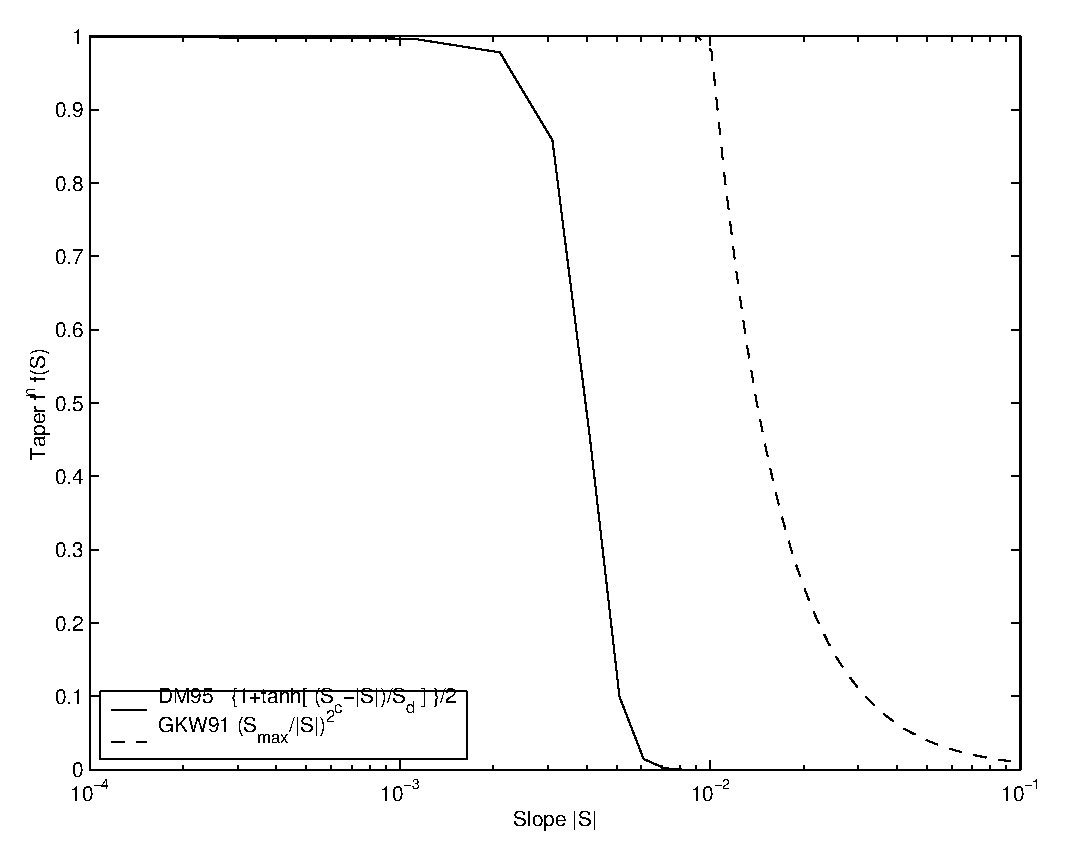
\includegraphics{part6/tapers.eps}}
\end{center}
\caption{Taper functions used in GKW99 and DM95.}
\label{fig:tapers}
\end{figure}

\begin{figure}
\begin{center}
\resizebox{5.0in}{3.0in}{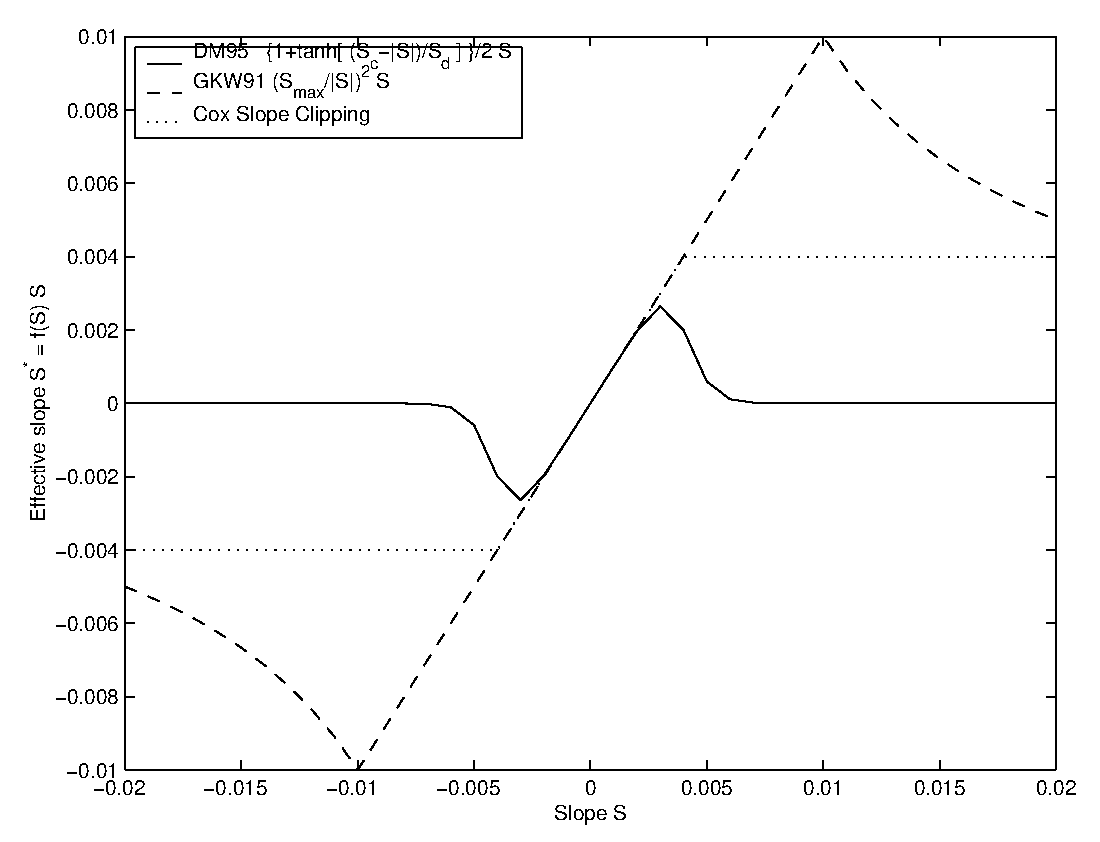
\includegraphics{part6/effective_slopes.eps}}
\end{center}
\caption{Effective slope as a function of ``true'' slope using Cox
slope clipping, GKW91 limiting and DM95 limiting.}
\label{fig:effective_slopes}
\end{figure}


\subsubsection{Slope clipping}

Deep convection sites and the mixed layer are indicated by
homogenized, unstable or nearly unstable stratification. The slopes in
such regions can be either infinite, very large with a sign reversal
or simply very large. From a numerical point of view, large slopes
lead to large variations in the tensor elements (implying large bolus
flow) and can be numerically unstable. This was first recognized by
Cox, 1987, who implemented ``slope clipping'' in the isopycnal mixing
tensor. Here, the slope magnitude is simply restricted by an upper
limit:
\begin{eqnarray}
|\nabla \sigma| & = & \sqrt{ \sigma_x^2 + \sigma_y^2 } \\
S_{lim} & = & - \frac{|\nabla \sigma|}{ S_{max} }
\;\;\;\;\;\;\;\; \mbox{where $S_{max}$ is a parameter} \\
\sigma_z^\star & = & \min( \sigma_z , S_{lim} ) \\
{[s_x,s_y]} & = & - \frac{ [\sigma_x,\sigma_y] }{\sigma_z^\star}
\end{eqnarray}
Notice that this algorithm assumes stable stratification through the
``min'' function. In the case where the fluid is well stratified ($\sigma_z < S_{lim}$) then the slopes evaluate to:
\begin{equation}
{[s_x,s_y]} = - \frac{ [\sigma_x,\sigma_y] }{\sigma_z}
\end{equation}
while in the limited regions ($\sigma_z > S_{lim}$) the slopes become:
\begin{equation}
{[s_x,s_y]} = \frac{ [\sigma_x,\sigma_y] }{|\nabla \sigma|/S_{max}}
\end{equation}
so that the slope magnitude is limited $\sqrt{s_x^2 + s_y^2} =
S_{max}$.

The slope clipping scheme is activated in the model by setting {\bf
GM\_tap\-er\_scheme = 'clipping'} in {\em data.gmredi}.

Even using slope clipping, it is normally the case that the vertical
diffusion term (with coefficient $\kappa_\rho{\bf K}_{33} =
\kappa_\rho S_{max}^2$) is large and must be time-stepped using an
implicit procedure (see section on discretisation and code later).
Fig. \ref{fig-mixedlayer} shows the mixed layer depth resulting from
a) using the GM scheme with clipping and b) no GM scheme (horizontal
diffusion). The classic result of dramatically reduced mixed layers is
evident. Indeed, the deep convection sites to just one or two points
each and are much shallower than we might prefer. This, it turns out,
is due to the over zealous re-stratification due to the bolus transport
parameterization. Limiting the slopes also breaks the adiabatic nature
of the GM/Redi parameterization, re-introducing diabatic fluxes in
regions where the limiting is in effect.

\subsubsection{Tapering: Gerdes, Koberle and Willebrand, Clim. Dyn. 1991}

The tapering scheme used in Gerdes et al., 1999, (\cite{gkw:99})
addressed two issues with the clipping method: the introduction of
large vertical fluxes in addition to convective adjustment fluxes is
avoided by tapering the GM/Redi slopes back to zero in
low-stratification regions; the adjustment of slopes is replaced by a
tapering of the entire GM/Redi tensor. This means the direction of
fluxes is unaffected as the amplitude is scaled.

The scheme inserts a tapering function, $f_1(S)$, in front of the
GM/Redi tensor:
\begin{equation}
f_1(S) = \min \left[ 1, \left( \frac{S_{max}}{|S|}\right)^2 \right]
\end{equation}
where $S_{max}$ is the maximum slope you want allowed. Where the
slopes, $|S|<S_{max}$ then $f_1(S) = 1$ and the tensor is un-tapered
but where $|S| \ge S_{max}$ then $f_1(S)$ scales down the tensor so
that the effective vertical diffusivity term $\kappa f_1(S) |S|^2 =
\kappa S_{max}^2$.

The GKW tapering scheme is activated in the model by setting {\bf
GM\_tap\-er\_scheme = 'gkw91'} in {\em data.gmredi}.

\subsection{Tapering: Danabasoglu and McWilliams, J. Clim. 1995}

The tapering scheme used by Danabasoglu and McWilliams, 1995,
\cite{dm:95}, followed a similar procedure but used a different
tapering function, $f_1(S)$:
\begin{equation}
f_1(S) = \frac{1}{2} \left( 1+\tanh \left[ \frac{S_c - |S|}{S_d} \right] \right)
\end{equation}
where $S_c = 0.004$ is a cut-off slope and $S_d=0.001$ is a scale over
which the slopes are smoothly tapered. Functionally, the operates in
the same way as the GKW91 scheme but has a substantially lower
cut-off, turning off the GM/Redi SGS parameterization for weaker
slopes.

The DM tapering scheme is activated in the model by setting {\bf
GM\_tap\-er\_scheme = 'dm95'} in {\em data.gmredi}.

\subsection{Tapering: Large, Danabasoglu and Doney, JPO 1997}

The tapering used in Large et al., 1997, \cite{ldd:97}, is based on the
DM95 tapering scheme, but also tapers the scheme with an additional
function of height, $f_2(z)$, so that the GM/Redi SGS fluxes are
reduced near the surface:
\begin{equation}
f_2(S) = \frac{1}{2} \left( 1 + \sin(\pi \frac{z}{D} - \pi/2)\right)
\end{equation}
where $D = L_\rho |S|$ is a depth-scale and $L_\rho=c/f$ with
$c=2$~m~s$^{-1}$.  This tapering with height was introduced to fix
some spurious interaction with the mixed-layer KPP parameterization.

The LDD tapering scheme is activated in the model by setting {\bf
GM\_tap\-er\_scheme = 'ldd97'} in {\em data.gmredi}.




\begin{figure}
\begin{center}
%\includegraphics{mixedlayer-cox.eps}
%\includegraphics{mixedlayer-diff.eps}
Figure missing.
\end{center}
\caption{Mixed layer depth using GM parameterization with a) Cox slope
clipping and for comparison b) using horizontal constant diffusion.}
\label{fig-mixedlayer}
\end{figure}






\newpage
\subsection{KPP Package: Ocean vertical mixing -- 
the nonlocal K-profile parameterization scheme}

\label{sec:pkg:kpp}
\begin{rawhtml}
<!-- CMIREDIR:package_kpp: -->
\end{rawhtml}


\newpage
% \documentclass[12pt]{article}
% \usepackage{amssymb}

%%%%%%%%%%%%%%%%%%%%%%%%%%%%%%%%%%%%%%%%%%%
%%  \usepackage{graphics}


% \oddsidemargin -4mm \evensidemargin 0mm
% \textwidth 165mm
% \textheight 230mm
% \topmargin -2mm \headsep -2mm
% \renewcommand{\baselinestretch}{1.5}
% \begin{document}


\def\deg{$^o$}
%%%--------------------------------------%%%
\section{THSICE: The Thermodynamic Sea Ice Package}
\label{sec:pkg:thsice}
\begin{rawhtml}
<!-- CMIREDIR:package_thsice: -->
\end{rawhtml}

{\bf Important note:}
This document has been written by Stephanie Dutkiewicz
and describes an earlier implementation of the sea-ice package.
This needs to be updated to reflect the recent changes (JMC).

\noindent
This thermodynamic ice model is based on the 3-layer model by Winton (2000).
and the energy-conserving LANL CICE model (Bitz and Lipscomb, 1999).
The model considers two equally thick ice layers; the upper layer has
a variable specific heat resulting from brine pockets,
the lower layer has a fixed heat capacity. A zero heat capacity snow
layer lies above the ice. Heat fluxes at the top and bottom
surfaces are used to calculate the change in ice and snow layer
thickness. Grid cells of the ocean model are 
either fully covered in ice or are open water. There is
a provision to parametrize ice fraction (and leads) in this package.
Modifications are discussed in small font following the
subroutine descriptions.

%%%%%%%%%%%%%%%%%%%%%%%%%%%%%%%%%%%%%%%%%%%%%%%%%%%%%%%%%%%%%%

\vspace{1cm}

\noindent
The ice model is called from {\it thermodynamics.F}, subroutine
{\it ice\_forcing.F} is called in place of {\it external\_forcing\_surf.F}.

%%%%%%%%%%%%%%%%%%%%%%%%%%%%%%%%%%%%%%%%%%%%%%%%%%%%%%%%%%%%%%

\vspace{1cm}
\noindent
{\bf \underline{subroutine ICE\_FORCING}}

\noindent
In {\it ice\_forcing.F}, we calculate the freezing potential of the
ocean model surface layer of water:
\[
  {\bf frzmlt} = (T_f - SST) \frac{c_{sw} \rho_{sw} \Delta z}{\Delta t}
\]
where $c_{sw}$ is seawater heat capacity, 
$\rho_{sw}$ is the seawater density, $\Delta z$
is the ocean model upper layer thickness and $\Delta t$ is the model (tracer)
timestep. The freezing temperature, $T_f=\mu S$ is a function of the
salinity.


1) Provided there is no ice present and {\bf frzmlt} is less than 0,
   the surface tendencies of wind, heat and freshwater are calculated
   as usual (ie. as in {\it external\_forcing\_surf.F}).

2) If there is ice present in the grid cell
   we call the main ice model routine {\it ice\_therm.F} (see below).
   Output from this routine gives net heat and freshwater flux 
   affecting the top of the ocean.

Subroutine {\it ice\_forcing.F} uses these values to find the 
sea surface tendencies
in grid cells. When there is ice present,  
the surface stress tendencies are
set to zero; the ice model is purely thermodynamic and the
effect of ice motion on the sea-surface is not examined.

Relaxation of surface $T$ and $S$ is only allowed equatorward
of {\bf relaxlat} (see {\bf DATA.ICE below}), and no relaxation is
allowed under the ice at any latitude.

\noindent
{\tiny (Note that there is provision for allowing grid cells to have both
open water and seaice; if {\bf compact} is between  0 and 1)}

%%%%%%%%%%%%%%%%%%%%%%%%%%%%%%%%%%%%%%%%%%%%%%%%%%%%%%%%%%%%%%
\vspace{1cm}
\noindent
{\bf {\underline{ subroutine ICE\_FREEZE}}}

This routine is called from {\it thermodynamics.F}
after the new temperature calculation, {\it calc\_gt.F}, 
but before {\it calc\_gs.F}.
In {\it ice\_freeze.F}, any ocean upper layer grid cell
with no ice cover, but with temperature below freezing,
$T_f=\mu S$ has ice initialized.
We calculate {\bf frzmlt} from all the grid cells in
the water column that have a temperature less than
freezing. In this routine, any water below the surface
that is below freezing is set to $T_f$.
A call to
{\it ice\_start.F} is made if {\bf frzmlt} $>0$, 
and salinity tendancy is updated for brine release.

\noindent
{\tiny (There is a provision for fractional ice:
In the case where the grid cell has less ice coverage than
{\bf icemaskmax} we allow {\it ice\_start.F} to be called).}

%%%%%%%%%%%%%%%%%%%%%%%%%%%%%%%%%%%%%%%%%%%%%%%%%%%%%%%%%%%%%%%%%%%

\vspace{1cm}
\noindent
{\bf {\underline{ subroutine ICE\_START}}}

\noindent
The energy available from freezing
the sea surface is brought into this routine as {\bf esurp}.
The enthalpy of the 2 layers of any new ice is calculated as:
\begin{eqnarray}
q_1 & = & -c_{i}*T_f + L_i \nonumber \\
q_2 & = & -c_{f}T_{mlt}+ c_{i}(T_{mlt}-T{f}) + L_i(1-\frac{T_{mlt}}{T_f} 
\nonumber \\
\end{eqnarray}
where  $c_f$ is specific heat of liquid fresh water, $c_i$ is the
specific heat of fresh ice, $L_i$ is latent heat of freezing, 
$\rho_i$ is density of ice and
$T_{mlt}$ is melting temperature of ice with salinity of 1.
The height of a new layer of ice is
\[
  h_{i new} = \frac{{\bf esurp} \Delta t}{qi_{0av}}
\]
where $qi_{0av}=-\frac{\rho_i}{2} (q_1+q_2)$.

The surface skin temperature $T_s$ and ice temperatures
$T_1$, $T_2$ and the sea surface temperature are set at $T_f$.

\noindent
{\tiny ( There is provision for fractional ice:
new ice is formed over open water; the first freezing in the cell
must have a height of {\bf himin0}; this determines the ice
fraction {\bf compact}. If there is already ice in the grid cell,
the new ice must have the same height and the new ice fraction
is 
\[
i_f=(1-\hat{i_f}) \frac{h_{i new}}{h_i}
\]
where $\hat{i_f}$ is ice fraction from previous timestep
and $h_i$ is current ice height. Snow is redistributed 
over the new ice fraction. The ice fraction is
not allowed to become larger than {\bf iceMaskmax} and
if the ice height is above {\bf hihig} then freezing energy
comes from the full grid cell,  ice growth does not occur
under orginal ice due to freezing water.
}
%%%%%%%%%%%%%%%%%%%%%%%%%%%%%%%%%%%%%%%%%%%%%%%%%%%%%%%%%%%%%%%%%%%

\vspace{1cm}
\noindent
{\bf {\underline{subroutine ICE\_THERM}}}

\noindent
The main subroutine of this package is {\it ice\_therm.F} where the
ice temperatures are calculated and the changes in ice and snow
thicknesses are determined. Output provides the net heat and fresh 
water fluxes that force the top layer of the ocean model.

If the current ice height is less than {\bf himin} then
the ice layer is set to zero and the ocean model upper layer temperature
is allowed to drop lower than its freezing temperature; and atmospheric
fluxes are allowed to effect the grid cell.
If the ice height is greater than  {\bf himin} we proceed with
the ice model calculation.

We follow the procedure
of Winton (1999) -- see equations 3 to 21 -- to calculate
the surface and internal ice temperatures. 
The surface temperature is found from the balance of the
flux at the surface $F_s$, the shortwave heat flux absorbed by the ice, 
{\bf fswint}, and
the upward conduction of heat through the snow and/or ice, $F_u$.
We linearize $F_s$ about the surface temperature, $\hat{T_s}$, 
at the previous timestep (where \mbox{}$\hat{ }$ indicates the value at
the  previous timestep):
\[
F_s (T_s) = F_s(\hat{T_s}) + \frac{\partial F_s(\hat{T_s)}}{\partial T_s}
(T_s-\hat{T_s})
\]
where, 
\[
F_s  =  F_{sensible}+F_{latent}+F_{longwave}^{down}+F_{longwave}^{up}+ (1-
\alpha) F_{shortwave}
\]
and
\[
 \frac{d F_s}{dT} = \frac{d F_{sensible}}{dT} + \frac{d F_{latent}}{dT}
+\frac{d F_{longwave}^{up}}{dT}.
\]
$F_s$ and $\frac{d F_s}{dT}$ are currently calculated from the {\bf BULKF} 
package described separately, but could also be provided by an atmospheric
model. The surface albedo is calculated from the ice height and/or 
surface temperature (see below, {\it srf\_albedo.F}) and the 
shortwave flux absorbed in the ice is
\[
{\bf fswint} = (1-e^{\kappa_i h_i})(1-\alpha) F_{shortwave}
\]
where $\kappa_i$ is bulk extinction coefficient.

The conductive flux to the surface is
\[
F_u=K_{1/2}(T_1-T_s)
\]
where $K_{1/2}$ is the effective conductive coupling of the snow-ice
layer between the surface and the mid-point of the upper layer of ice
$
K_{1/2}=\frac{4 K_i K_s}{K_s h_i + 4 K_i h_s}
$.
$K_i$ and $K_s$ are constant thermal conductivities of seaice and snow.

From the above equations we can develop a system of equations to
find the skin surface temperature, $T_s$ and the two ice layer
temperatures (see Winton, 1999, for details). We solve these
equations iteratively until the change in $T_s$ is small.
When the surface temperature is greater then
the melting temperature of the surface, the temperatures are
recalculated setting $T_s$ to 0.  The enthalpy
of the ice layers are calculated in order to keep track of the energy in the
ice model. Enthalpy is defined, here, as the energy required to melt a
unit mass of seaice with temperature $T$.
For the upper layer (1) with brine pockets  and
the lower fresh layer (2):
\begin{eqnarray}
q_1 & = & - c_f T_f + c_i (T_f-T)+ L_{i}(1-\frac{T_f}{T})
\nonumber \\
q_2 & = & -c_i T+L_i \nonumber
\end{eqnarray}
where $c_f$ is specific heat of liquid fresh water, $c_i$ is the
specific heat of fresh ice, and $L_i$ is latent heat of melting fresh ice.



From the new ice temperatures, we can calculate
the energy flux at the surface available for melting (if $T_s$=0)
and the energy at the ocean-ice interface for either melting or freezing.
\begin{eqnarray}
E_{top} &  =  & (F_s- K_{1/2}(T_s-T_1) ) \Delta t
\nonumber \\
E_{bot} &= & (\frac{4K_i(T_2-T_f)}{h_i}-F_b) \Delta t
\nonumber
\end{eqnarray}
where $F_b$ is the heat flux at the ice bottom due to the sea surface
temperature variations from freezing.
If $T_{sst}$ is above freezing, $F_b=c_{sw} \rho_{sw} 
\gamma (T_{sst}-T_f)u^{*}$, $\gamma$ is the heat transfer coefficient
and $u^{*}=QQ$ is frictional velocity between ice 
and water. If $T_{sst}$ is below freezing,
$F_b=(T_f - T_{sst})c_f \rho_f \Delta z /\Delta t$ and set $T_{sst}$
to $T_f$. We also
include the energy from lower layers that drop below freezing,
and set those layers to $T_f$.

If $E_{top}>0$ we melt snow from the surface, if all the snow is melted
and there is energy left, we melt the ice. If the ice is all gone
and there is still energy left, we apply the left over energy to 
heating the ocean model upper layer (See Winton, 1999, equations 27-29).
Similarly if $E_{bot}>0$ we melt ice from the bottom. If all the ice
is melted, the snow is melted (with energy from the ocean model upper layer
if necessary). If $E_{bot}<0$ we grow ice at the bottom
\[
\Delta h_i = \frac{-E_{bot}}{(q_{bot} \rho_i)}
\]
where $q_{bot}=-c_{i} T_f + L_i$ is the enthalpy of the new ice,
The enthalpy of the second ice layer, $q_2$ needs to be modified:
\[
q_2 = \frac{ \hat{h_i}/2 \hat{q_2} + \Delta h_i q_{bot} }
        {\hat{h_i}/{2}+\Delta h_i}
\]

If there is a ice layer and the overlying air temperature is
below 0$^o$C then any precipitation, $P$ joins the snow layer:
\[
\Delta h_s  = -P \frac{\rho_f}{\rho_s} \Delta t, 
\]
$\rho_f$ and $\rho_s$ are the fresh water and snow densities.
Any evaporation, similarly, removes snow or ice from the surface.
We also calculate the snow age here, in case it is needed for
the surface albedo calculation (see {\it srf\_albedo.F} below).

For practical reasons we limit the ice growth to {\bf hilim}
and snow is limited to {\bf hslim}. We converts any
ice and/or snow above these limits back to water, maintaining the salt
balance. Note however, that heat is not conserved in this
conversion; sea surface temperatures below the ice are not
recalculated.

If the snow/ice interface is below the waterline, snow is converted
to ice (see Winton, 1999, equations 35 and 36). The subroutine
{\it new\_layers\_winton.F}, described below, repartitions the ice into
equal thickness layers while conserving energy.

The subroutine {\it ice\_therm.F} now calculates the heat and fresh
water fluxes affecting the ocean model surface layer. The heat flux:
\[
q_{net}= {\bf fswocn} - F_{b} - \frac{{\bf esurp}}{\Delta t}
\]
is composed of the shortwave flux that has passed through the
ice layer and is absorbed by the water, {\bf fswocn}$=QQ$,
the ocean flux to the ice $F_b$,
and the surplus energy left over from the melting, {\bf esurp}.
The fresh water flux is determined from the amount of
fresh water and salt in the ice/snow system before and after the
timestep.

\noindent
{\tiny (There is a provision for fractional ice:
If ice height is above {\bf hihig} then all energy from freezing at
sea surface is used only in the open water aparts of the cell (ie.
$F_b$ will only have the conduction term).
The melt energy is partitioned by {\bf frac\_energy} between melting
ice height and ice extent. However, once ice height drops below
{\bf himon0} then all energy melts ice extent.}

%%%%%%%%%%%%%%%%%%%%%%%%%%%%%%%%%%%%%%%%%%%%%%%%%%%%%%%%%%%%%%%
\vspace{1cm}

\noindent
{\bf {\underline{subroutine SFC\_ALBEDO} } }

\noindent
The routine {\it ice\_therm.F} calls this routine to determine
the surface albedo. There are two calculations provided here:

\noindent
{\bf 1)} from LANL CICE model
\[ \alpha = f_s \alpha_s + (1-f_s) (\alpha_{i_{min}}
         + (\alpha_{i_{max}}- \alpha_{i_{min}}) (1-e^{-h_i/h_{\alpha}}))
\]
where $f_s$ is 1 if there is snow, 0 if not; the snow albedo, 
$\alpha_s$ has two values
depending on whether $T_s<0$ or not; $\alpha_{i_{min}}$ and 
$\alpha_{i_{max}}$ are ice albedos for thin melting ice, and
thick bare ice respectively, and $h_{\alpha}$ is a scale
height.

\noindent
{\bf 2)} From GISS model (Hansen et al 1983)
\[
 \alpha = \alpha_i e^{-h_s/h_a} + \alpha_s (1-e^{-h_s/h_a})
\]
where $\alpha_i$ is a constant albedo for bare ice, $h_a$
is a scale height and $\alpha_s$ is a variable snow albedo.
\[
\alpha_s = \alpha_1 + \alpha_2 e^{-\lambda_a a_s}
\]
where $\alpha_1$ is a constant, $\alpha_2$ depends on $T_s$,
$a_s$ is the snow age, and $\lambda_a$ is a scale frequency.
The snow age is calculated in {\it ice\_therm.F} and is given
in equation 41 in Hansen et al (1983).

%%%%%%%%%%%%%%%%%%%%%%%%%%%%%%%%%%%%%%%%%%%%%%%%%%%%%%%%%%%%%%%

\vspace{1cm}

\noindent
{\bf {\underline{subroutine NEW\_LAYERS\_WINTON}}}

\noindent
The subroutine
{\it new\_layers\_winton.F} repartitions the ice into
equal thickness layers while conserving energy. We pass
to this subroutine, the ice layer enthalpies after
melting/growth and the new height of the ice layers.
The ending layer height should be half the sum of the
new ice heights from {\it ice\_therm.F}. The enthalpies
of the ice layers are adjusted accordingly to maintain
total energy in the ice model. If layer 2 height is
greater than layer 1 height then layer 2 gives ice to
layer 1 and:
\[
q_1=f_1 \hat{q_1} + (1-f1) \hat{q_2}
\]
where $f_1$ is the fraction of the new to old upper layer heights.
$T_1$ will therefore also have changed.
Similarly for when ice layer height 2 is less than
layer 1 height, except here we need to to be careful
that the new $T_2$ does not fall below the melting temperature.

%%%%%%%%%%%%%%%%%%%%%%%%%%%%%%%%%%%%%%%%%%%%%%%%%%%%%%%%%%%%%%%

\vspace{1cm}

\noindent
{\bf {\underline{Initializing subroutines}}}

\noindent
{\it ice\_init.F}:
Set ice variables to zero, or reads in pickup information
from {\bf pickup.ic} (which was written out in {\it checkpoint.F})

\noindent
{\it ice\_readparms.F}:
Reads {\bf data.ice}

%%%%%%%%%%%%%%%%%%%%%%%%%%%%%%%%%%%%%%%%%%%%%%%%%%%%%%%%%%%%%%%

\vspace{1cm}

\noindent
{\bf {\underline{Diagnostic subroutines}}}

\noindent
{\it ice\_ave.F}:
Keeps track of means of the ice variables

\noindent
{\it ice\_diags.F}:
Finds averages and writes out diagnostics

%%%%%%%%%%%%%%%%%%%%%%%%%%%%%%%%%%%%%%%%%%%%%%%%%%%%%%%%%%%%%%%%
\vspace{1cm}

\noindent
{\bf {\underline{Common Blocks}}}

\noindent
{\it ICE.h}: Ice Varibles, also 
{\bf relaxlat} and {\bf startIceModel}

\noindent
{\it ICE\_DIAGS.h}: matrices for diagnostics: averages of fields
from {\it ice\_diags.F}

\noindent
{\it BULKF\_ICE\_CONSTANTS.h} (in {\bf BULKF} package): 
all the parameters need by the ice model

%%%%%%%%%%%%%%%%%%%%%%%%%%%%%%%%%%%%%%%%%%%%%%%%%%%%%%%%%%%%%%%%%%
\vspace{1cm}

\noindent
{\bf {\underline{Input file DATA.ICE}}}

\noindent
Here we need to set {\bf StartIceModel}: which is 1 if the
model starts from no ice; and 0 if there is a pickup file
with the ice matrices ({\bf pickup.ic}) which is read
in {\it ice\_init.F} and written out in {\it checkpoint.F}.
The parameter {\bf relaxlat} defines the latitude poleward
of which there is no relaxing of surface $T$ or $S$ to
observations. This avoids the relaxation forcing the ice
model at these high latitudes.

\noindent
({\tiny Note: {\bf hicemin} is set to 0 here. If the
provision for allowing grid cells to have both
open water and seaice is ever implemented, this would
be greater than 0})

%%%%%%%%%%%%%%%%%%%%%%%%%%%%%%%%%%%%%%%%%%%%%%%%%%%%%%%%%%%%
\vspace{1cm}

\noindent
{\bf {\underline{Important Notes}}}

\noindent
{\bf 1)} heat fluxes have different signs in the ocean and ice
models.

\noindent
{\bf 2)} {\bf StartIceModel} must be changed in {\bf data.ice}:
1 (if starting from no ice), 0 (if using pickup.ic file).

%%%%%%%%%%%%%%%%%%%%%%%%%%%%%%%%%%%%%%%%%%%%%%%%%%%%%%%%%%%%%%

\vspace{1cm}

\noindent 
{\bf {\underline{References}}}

\noindent
Bitz, C.M. and W.H. Lipscombe, 1999: An Energy-Conserving
Thermodynamic Model of Sea Ice.
{\it Journal of Geophysical Research}, 104, 15,669 -- 15,677.

\vspace{.2cm}

\noindent
Hansen, J., G. Russell, D. Rind, P. Stone, A. Lacis, S. Lebedeff,
R. Ruedy and L.Travis, 1983: Efficient Three-Dimensional
Global Models for Climate Studies: Models I and II.
{\it Monthly Weather Review}, 111, 609 -- 662.

\vspace{.2cm}

\noindent
Hunke, E.C and W.H. Lipscomb, circa 2001: CICE: the Los Alamos
Sea Ice Model Documentation and Software User's Manual.
LACC-98-16v.2.\\
(note: this documentation is no longer available as CICE has progressed
to a very different version 3)


\vspace{.2cm}

\noindent
Winton, M, 2000: A reformulated Three-layer Sea Ice Model.
{\it Journal of Atmospheric and Ocean Technology}, 17, 525 -- 531.



%%%%%%%%%%%%%%%%%%%%%%%%%%%%%%%%%%%%%%%%%%%
% \end{document}


\newpage
% \documentclass[12pt]{article}
% \usepackage{amssymb}
% 
% \usepackage{graphics}
% 
% 
% \oddsidemargin -4mm \evensidemargin 0mm
% \textwidth 165mm
% \textheight 230mm
% \topmargin -2mm \headsep -2mm
% \renewcommand{\baselinestretch}{1.5}
% \begin{document}
% 

%%%--------------------------------------%%%
\def\deg{$^o$}
\section{BULK\_FORCE: Bulk Formula Package}
\label{sec:pkg:bulk_formula}
\begin{rawhtml}
<!-- CMIREDIR:package_bulk_formula: -->
\end{rawhtml}

author: Stephanie Dutkiewicz\\

\noindent
Instead of forcing the model with heat and fresh water flux data,
this package calculates these fluxes using the changing sea surface
temperature. We need to read in some atmospheric data:
{\bf air temperature, air humidity, down shortwave radiation,
     down longwave radiation, precipitation, wind speed}.
The current setup also reads in {\bf wind stress}, but this
can be changed so that the stresses are calculated from the
wind speed.

The current setup requires that there is the thermodynamic-seaice package
({\it pkg/thsice}, also refered below as seaice)
is also used. It would be useful though to have it also
setup to run with some very simple parametrization of the sea ice.

%%%%%%%%%%%%%%%%%%%%%%%%%%%%%%%%%%%%%%%%%%%%%%%%%%%%%%%%%%%%%%

\vspace{1cm}

\noindent
The heat and fresh water fluxes are calculated in {\it bulkf\_forcing.F}
called from {\it forward\_step.F}. These fluxes are used over open water,
fluxes over seaice are recalculated in the sea-ice package.
Before the call to {\it bulkf\_forcing.F} we call 
{\it bulkf\_fields\_load.F} to find the current atmospheric conditions.
The only other changes to the model code come from the initializing
and writing diagnostics of these fluxes.

%%%%%%%%%%%%%%%%%%%%%%%%%%%%%%%%%%%%%%%%%%%%%%%%%%%%%%%%%%%%%%
\vspace{1cm}
\noindent
{\bf \underline{subroutine BULKF\_FIELDS\_LOAD}}

\noindent
Here we find the atmospheric data needed for the bulk formula
calculations. These are read in at periodic intervals and
values are interpolated to the current time. The data file names
come from {\bf data.blk}. The values that can be read in are:
air temperature, air humidity, precipitation, 
down solar radiation, down long
wave radiation, zonal and meridional wind speeds, total wind
speed, net heat flux, net freshwater forcing, cloud cover,
snow fall, zonal and meridional wind stresses, and SST and SSS
used for relaxation terms.
Not all these files are necessary or used. For instance cloud
cover and snow fall are not used in the current bulk formula
calculation. If total wind speed is not supplied, wind speed
is calculate from the zonal and meridional components. If
wind stresses are not read in, then the stresses are calculated
from the wind speed. Net heat flux and net freshwater can be
read in and used over open ocean instead of the bulk formula
calculations (but over seaice the bulkf formula is always
used). This is "hardwired" into {\it bulkf\_forcing} and
the "ch" in the variable names suggests that this is "cheating".
SST and SSS need to be read in if there is any relaxation used.


%%%%%%%%%%%%%%%%%%%%%%%%%%%%%%%%%%%%%%%%%%%%%%%%%%%%%%%%%%%%%%


\vspace{1cm}
\noindent
{\bf \underline{subroutine BULKF\_FORCING}}

\noindent
In {\it bulkf\_forcing.F}, we calculate  heat and fresh water
fluxes (and wind stress, if necessary) for each grid cell.
First we determine if the grid cell is open water or seaice
and this information is carried by {\bf iceornot}. There is
a provision here for a different designation if there is
snow cover (but currently this does not make any difference).
We then call {\it bulkf\_formula\_lanl.F} which provides
values for: up long wave radiation, latent and sensible heat
fluxes, the derivative of these three with respect to surface
temperature, wind stress, evaporation. 
Net long wave radiation is calculated from the combination
of the down long wave read in and the up long wave calculated.

We then find the albedo of the surface - with a call to
{\it sfc\_albedo} if there is sea-ice (see the seaice package
for information on the subroutine). If the grid cell is open
ocean the albedo is set as 0.1. Note that this is a parameter
that can be used to tune the results. The net short wave
radiation is then the down shortwave radiation minus the 
amount reflected.

If the wind stress needed to be calculated in {\it bulkf\_formula\_lanl.F},
it was calculated to grid cell center points, so in {\it bulkf\_forcing.F}
we regrid to {\bf u} and {\bf v} points. We let the model know
if it has read in stresses or calculated stresses by the switch
{\bf readwindstress} which is can be set in data.blk, and defaults
to {\bf .TRUE.}.

We then calculate {\bf Qnet} and {\bf EmPmR} that will be used
as the fluxes over the open ocean. There is a provision for
using runoff. If we are "cheating" and using observed fluxes 
over the open ocean, then there is a provision here to
use read in {\bf Qnet} and {\bf EmPmR}.

The final call is to calculate averages of the terms found
in this subroutine.

%%%%%%%%%%%%%%%%%%%%%%%%%%%%%%%%%%%%%%%%%%%%%%%%%%%%%%%%%%%%%%
\vspace{1cm}
\noindent
{\bf {\underline{ subroutine BULKF\_FORMULA\_LANL}}}

\noindent
This is the main program of the package where the
heat fluxes and freshwater fluxes over ice and
open water are calculated. Note that this subroutine
is also called from the seaice package during the
iterations to find the ice surface temperature.

Latent heat ($L$) used in this subroutine 
depends on the state of the surface: vaporization for
open water, fusion and vaporization for ice surfaces.
Air temperature is converted from Celsius to Kelvin.
If there is no wind speed ($u_s$) given, then the wind speed
is calculated from the zonal and meridional components.

We calculate the virtual temperature:
\[
T_o = T_{air} (1+\gamma q_{air})
\]
where $T_{air}$ is the air temperature at $h_T$, $q_{air}$ is
humidity at $h_q$ and $\gamma$ is a constant.

The saturated vapor pressure is calculate (QQ ref):
\[
q_{sat} = \frac{a}{p_o} e^{L (b-\frac{c}{T_{srf}})}
\]
where $a,b,c$ are constants, $T_{srf}$ is surface temperature
and $p_o$ is the surface pressure.

The two values crucial for the bulk formula calculations are
the difference between air at sea surface and sea surface temperature:
\[
\Delta T = T_{air} - T_{srf} +\alpha h_T
\]
where $\alpha$ is adiabatic lapse rate and $h_T$ is the  height
where the air temperature was taken; and the difference
between the air humidity and the saturated humidity
\[
\Delta q = q_{air} - q_{sat}.
\]

We then calculate the turbulent exchange coefficients
following Bryan et al (1996) and the numerical scheme
of Hunke and Lipscombe (1998). 
We estimate initial values for the exchange coefficients, $c_u$,
$c_T$ and $c_q$ as
\[
\frac{\kappa}{ln(z_{ref}/z_{rou})}
\]
where $\kappa$ is the Von Karman constant, $z_{ref}$ is a
reference height and $z_{rou}$ is a roughness length scale
which could be a function of type of surface, but is here set
as a constant. Turbulent scales are:
\begin{eqnarray}
u^* & = & c_u u_s \nonumber\\
T^* & = & c_T \Delta T \nonumber\\
q^* & = & c_q \Delta q \nonumber
\end{eqnarray}

We find the "integrated flux profile" for momentum and stability
if there are stable QQ conditions ($\Upsilon>0$) :
\[
\psi_m = \psi_s = -5 \Upsilon
\]
and for unstable QQ conditions ($\Upsilon<0$):
\begin{eqnarray}
\psi_m & = & 2 ln(0.5(1+\chi)) + ln(0.5(1+\chi^2)) - 2 \tan^{-1} \chi + \pi/2
\nonumber \\
\psi_s & = & 2 ln(0.5(1+\chi^2)) \nonumber
\end{eqnarray}
where
\[
\Upsilon = \frac{\kappa g z_{ref}}{u^{*2}} (\frac{T^*}{T_o} + 
\frac{q^*}{1/\gamma + q_a})
\]
and $\chi=(1-16\Upsilon)^{1/2}$.

The coefficients are updated through 5 iterations as:
\begin{eqnarray}
c_u & = & \frac {\hat{c_u}}{1+\hat{c_u}(\lambda - \psi_m)/\kappa} \nonumber \\
c_T & = & \frac {\hat{c_T}}{1+\hat{c_T}(\lambda - \psi_s)/\kappa} \nonumber \\
c_q & = & c'_T
\end{eqnarray}
where $\lambda =ln(h_T/z_{ref})$.

We can then find the bulk formula heat fluxes:

\vspace{.2cm}
\noindent
Sensible heat flux:
\[
Q_s=\rho_{air} c_{p_{air}} u_s c_u c_T \Delta T
\]

\vspace{.2cm}
\noindent
Latent heat flux:
\[
Q_l=\rho_{air} L u_s c_u c_q \Delta q
\]

\vspace{.2cm}
\noindent
Up long wave radiation
\[
Q_{lw}^{up}=\epsilon \sigma T_{srf}^4
\]
where $\epsilon$ is emissivity (which can be different for
open ocean, ice and snow), $\sigma$ is Stefan-Boltzman constant.

We calculate the derivatives of the three above functions
with respect to surface temperature
\begin{eqnarray}
\frac{dQ_s}{d_T} & = & \rho_{air} c_{p_{air}} u_s c_u c_T \nonumber \\
\frac{dQ_l}{d_T} & = & \frac{\rho_{air} L^2 u_s c_u c_q c}{T_{srf}^2} \nonumber \\
\frac{dQ_{]lw}^{up}}{d_T} & = &  4 \epsilon \sigma t_{srf}^3 \nonumber
\end{eqnarray}

And total derivative $\frac{dQ_o}{dT}= \frac{dQ_s}{dT} +
\frac{dQ_l}{dT} + \frac{dQ_{lw}^{up}}{dT}$.




If we do not read in the wind stress, it is calculated here.

%%%%%%%%%%%%%%%%%%%%%%%%%%%%%%%%%%%%%%%%%%%%%%%%%%%%%%%%%%%%%%%

\vspace{1cm}

\noindent
{\bf {\underline{Initializing subroutines}}}

\noindent
{\it bulkf\_init.F}:
Set bulkf variables to zero.

\noindent
{\it bulkf\_readparms.F}:
Reads {\bf data.blk}

%%%%%%%%%%%%%%%%%%%%%%%%%%%%%%%%%%%%%%%%%%%%%%%%%%%%%%%%%%%%%%%

\vspace{1cm}

\noindent
{\bf {\underline{Diagnostic subroutines}}}

\noindent
{\it bulkf\_ave.F}:
Keeps track of means of the bulkf variables

\noindent
{\it bulkf\_diags.F}:
Finds averages and writes out diagnostics

%%%%%%%%%%%%%%%%%%%%%%%%%%%%%%%%%%%%%%%%%%%%%%%%%%%%%%%%%%%%%%%%
\vspace{1cm}

\noindent
{\bf {\underline{Common Blocks}}}

\noindent
{\it BULKF.h}: BULKF Variables,  data file names, and logicals
{\bf readwindstress} and {\bf readsurface}

\noindent
{\it BULKF\_DIAGS.h}: matrices for diagnostics: averages of fields
from {\it bulkf\_diags.F}

\noindent
{\it BULKF\_ICE\_CONSTANTS.h}: 
all the parameters need by the ice model and in the bulkf formula
calculations.

%%%%%%%%%%%%%%%%%%%%%%%%%%%%%%%%%%%%%%%%%%%%%%%%%%%%%%%%%%%%%%%%%%
\vspace{1cm}

\noindent
{\bf {\underline{Input file DATA.ICE}}}

\noindent
We read in the file names of atmospheric data used in
the  bulk formula calculations. Here we can also set
the logicals: {\bf readwindstress} if we read in the
wind stress rather than calculate it from the wind
speed; and {\bf readsurface} to read in the surface
temperature and salinity if these will be used as
part of a relaxing term.

%%%%%%%%%%%%%%%%%%%%%%%%%%%%%%%%%%%%%%%%%%%%%%%%%%%%%%%%%%%%
\vspace{1cm}

\noindent
{\bf {\underline{Important Notes}}}

\noindent
{\bf 1)} heat fluxes have different signs in the ocean and ice
models.

\noindent
{\bf 2)} {\bf StartIceModel} must be changed in {\bf data.ice}:
1 (if starting from no ice), 0 (if using pickup.ic file).

%%%%%%%%%%%%%%%%%%%%%%%%%%%%%%%%%%%%%%%%%%%%%%%%%%%%%%%%%%%%%%

\vspace{1cm}

\noindent 
{\bf {\underline{References}}}


\vspace{.2cm}

\noindent
Bryan F.O., B.G Kauffman, W.G. Large, P.R. Gent, 1996:
The NCAR CSM flux coupler. Technical note TN-425+STR,
NCAR.

\vspace{.2cm}

\noindent
Hunke, E.C and W.H. Lipscomb, circa 2001: CICE: the Los Alamos
Sea Ice Model Documentation and Software User's Manual.
LACC-98-16v.2.\\
(note: this documentation is no longer available as CICE has progressed
to a very different version 3)





%%%%%%%%%%%%%%%%%%%%%%%%%%%%%%%%%%%%%%%%%%%
% \end{document}


\newpage
% $Header: /u/gcmpack/manual/s_phys_pkgs/text/generic_advdiff.tex,v 1.3 2004/10/12 18:16:03 edhill Exp $
% $Name:  $


\section{Generic Advection/Diffusion}
\label{sec:pkg:gad}
\begin{rawhtml}
<!-- CMIREDIR:package_gad: -->
\end{rawhtml}

The {\tt generic\_advdiff} package provides...


\subsection{Introduction}
Package {\tt generic\_advdiff} is a...


\subsection{Key subroutines, parameters and files}
\label{sec:pkg:rw:implementation_synopsis}
The {\tt generic\_advdiff} package has... 




\newpage
\subsection{Atmospheric Intermediate Physics: AIM}
\label{sec:pkg:aim}
\begin{rawhtml}
<!-- CMIREDIR:package_aim: -->
\end{rawhtml}

Note:
 The folowing document below describes the \texttt{aim\_v23} package
 that is based on the version v23 of the SPEEDY code (\cite{molteni:03}).

\subsubsection{Key subroutines, parameters and files}
\label{sec:pkg:aim:implementation}


\newpage
\section{Land package}

This package provides a simple land model
based on Rong Zhang [e-mail:roz@gfdl.noaa.gov] 2 layers model
(see documentation below).

It is primarily implemented for AIM (\_v23) atmospheric physics
but could be adapted to work with a different atmospheric physics.
Two subroutines ({\it aim\_aim2land.F} {\it aim\_land2aim.F}
in {\it pkg/aim\_v23}) are used as interface with AIM physics. 

Number of layers is a parameter ({\it land\_nLev} in {\it LAND\_SIZE.h})
and can be changed. 

%---------------------------------------------------------------------

% \documentclass[12pt,thmsa]{article}

% \begin{document}

\begin{center}
{\bf Note on Land Model}\\
date: June 1999\\
author: Rong Zhang\\
\end{center}

% \baselineskip19pt

This is a simple 2-layer land model. The top layer depth $z1=0.1m$, the
second layer depth $z2=4m$.

Let $T_{g1},T_{g2}$ be the temperature of each layer, $W_{1,}W_{2}$ be the
soil moisture of each layer. The field capacity $f_{1,}$ $f_{2}$ are the
maximum water amount in each layer, so $W_{i}$ is the ratio of available
water to field capacity. $f_{i}=\gamma z_{i},\gamma =0.24$ is the field
capapcity per meter soil$,$ so $f_{1}=0.024m,$ $f_{2}=0.96m.$

The land temperature is determined by total surface downward heat flux $F,$

\begin{equation}
z_{1}C_{1}\frac{dT_{g1}}{dt}=F-\lambda \frac{T_{g1}-T_{g2}}{(z_{1}+z_{2})/2}
\end{equation}

\begin{center}
\begin{equation}
z_{2}C_{2}\frac{dT_{g2}}{dt}=\lambda \frac{T_{g1}-T_{g2}}{(z_{1}+z_{2})/2}
\end{equation}
\end{center}

here $C_{1},C_{2}$ are the heat capacity of each layer , $\lambda $ is the
thermal conductivity, $\lambda =0.42Wm^{-1}K^{-1}.$

\begin{center}
\bigskip 
\begin{equation}
C_{1}=C_{w}W_{1}\gamma +C_{s}
\end{equation}

\begin{equation}
C_{2}=C_{w}W_{2}\gamma +C_{s}
\end{equation}
\end{center}

$C_{w},C_{s}$ are the heat capacity of water and dry soil respectively. $%
C_{w}=4.2\times 10^{6}Jm^{-3}K^{-1},C_{s}=1.13\times 10^{6}Jm^{-3}K^{-1}.$

\bigskip

The soil moisture is determined by precipitation $P(m/s)$,surface
evaporation $E(m/s)$ and runoff $R(m/s).$

\begin{equation}
\frac{dW_{1}}{dt}=\frac{P-E-R}{f_{1}}+\frac{W_{2}-W_{1}}{\tau }
\end{equation}

$\tau =2$ $days$ is the time constant for diffusion of moisture between
layers.

\begin{equation}
\frac{dW_{2}}{dt}=\frac{f_{1}}{f_{2}}\frac{W_{1}-W_{2}}{\tau }
\end{equation}

In the code, $R=0$ gives better result, $W_{1},W_{2}$ are set to be within
[0, 1]. If $W_{1}$ is greater than 1, then let $\delta W_{1}=W_{1}-1,W_{1}=1$
and $W_{2}=W_{2}+p\delta W_{1}\frac{f_{1}}{f_{2}}$, i.e. the runoff of top
layer is put into second layer. $p=0.5$ is the fraction of top layer runoff
that is put into second layer.

The time step is 1 hour, it takes several years to reach equalibrium offline.

\begin{center}
\bigskip
\end{center}

\textbf{References}

Hansen J. et al. Efficient three-dimensional global models for climate
studies: models I and II. \emph{Monthly Weather Review}, vol.111, no.4, pp.
609-62, 1983

% \end{document}


\newpage
\section{Coupling interface for Atmospheric Intermediate code}
\label{sec:aim_compon_interf}
\subsection{Key subroutines, parameters and files}
\label{sec:pkg:aim_compon_interf:implementation_synopsis}
\subsection{Package Reference}


\newpage
\section{Coupler for mapping between AIM and ocean }
\label{sec:pkg:aim_ocn_coupler}
\begin{rawhtml}
<!-- CMIREDIR:package_aim_ocn_coupler: -->
\end{rawhtml}

\subsection{Key subroutines, parameters and files}
\label{sec:pkg:aim_ocn_coupler:implementation_synopsis}


\newpage
\subsection{Toolkit for building couplers}
\label{sec:component_communications}
\label{sec:pkg:component_communications}
\begin{rawhtml}
<!-- CMIREDIR:package_component_communications: -->
\end{rawhtml}

\subsubsection{Key subroutines, parameters and files}
\label{sec:pkg:component_communications:implementation_synopsis}

\subsubsection{Experiments and tutorials that use component\_communications}
\label{sec:pkg:component_communications:experiments}

\begin{itemize}
\item{Global coupled ocean atmosphere experiment in cpl\_aim+ocean verification directory. }
\end{itemize}


\newpage
% $Header: /u/gcmpack/manual/s_phys_pkgs/Attic/mnc.tex,v 1.12 2004/10/12 18:16:03 edhill Exp $
% $Name:  $

\section{NetCDF I/O Integration: MNC}
\label{sec:pkg:mnc}
\begin{rawhtml}
<!-- CMIREDIR:package_mnc: -->
\end{rawhtml}

The \texttt{mnc} package is a set of convenience routines written to
expedite the process of creating, appending, and reading NetCDF files.
NetCDF is an increasingly popular self-describing file format
\cite{rew:97} intended primarily for scientific data sets.  An
extensive collection of NetCDF reference papers, user guides,
software, FAQs, and other information can be obtained from UCAR's web
site at:
\begin{rawhtml} <A href="http://www.unidata.ucar.edu/packages/netcdf/"> \end{rawhtml}
\begin{verbatim}
http://www.unidata.ucar.edu/packages/netcdf/
\end{verbatim}
\begin{rawhtml} </A> \end{rawhtml}


\subsection{Using MNC}

\subsubsection{MNC Configuration and Inputs}

As with all MITgcm packages, MNC can be turned on/off at compile time
using the \texttt{packages.conf} file or the genmake2
\texttt{-enable=mnc} or \texttt{-disable=mnc} switches.

For run-time configuration, most of the MNC--related model parameters
are contained within a Fortran namelist file called \texttt{data.mnc}.
If this file does not exist, then the MNC package will interpret that
as an indication that it is not to be used.  If the \texttt{data.mnc}
file does exist, then it may contain the following parameters:

\begin{center}
  {\footnotesize
    \begin{tabular}[htb]{|l|c|l|l|}\hline
      \textbf{Name}  &  \textbf{T}  &  
      \textbf{Default}  &  \textbf{Description}  \\\hline
      &  &  &  \\
      \texttt{useMNC}  &  L  & \texttt{.FALSE.}  &  
      \textbf{overall MNC ON/OFF switch}  \\
      \texttt{mnc\_echo\_gvtypes}  &  L  & \texttt{.FALSE.}  &  
      echo pre-defined ``types'' (debugging)   \\
      \texttt{mnc\_use\_outdir}  &  L  & \texttt{.FALSE.}  &  
      create a directory for output  \\
      \texttt{mnc\_outdir\_str}  &  S  & \texttt{'mnc\_'}  &  
      output directory name \\
      \texttt{mnc\_outdir\_date}  &  L  & \texttt{.FALSE.}  &  
      embed date in the output dir name  \\
      \texttt{pickup\_write\_mnc}  &  L  & \texttt{.FALSE.}  &  
      use MNC to write (create) pickup files  \\
      \texttt{pickup\_read\_mnc}  &  L  & \texttt{.FALSE.}  &  
      use MNC to read pickup files  \\
      \texttt{mnc\_use\_indir}  &  L  & \texttt{.FALSE.}  &  
      use a directory (path) for input  \\
      \texttt{mnc\_indir\_str}  &  S  & \texttt{''}  &  
      input directory (or path) name  \\
      \texttt{snapshot\_mnc}  &  L  & \texttt{.FALSE.}  &  
      write \texttt{snapshot} (instantaneous) w/MNC  \\
      \texttt{monitor\_mnc}  &  L  & \texttt{.FALSE.}  &  
      write \texttt{monitor} w/MNC  \\
      \texttt{timeave\_mnc}  &  L  & \texttt{.FALSE.}  &  
      write \texttt{timeave} w/MNC  \\
      \texttt{autodiff\_mnc}  &  L  & \texttt{.FALSE.}  &  
      write \texttt{autodiff} w/MNC  \\\hline
    \end{tabular}
  }
\end{center}

Additional MNC--related parameters are contained within the main
\texttt{data} namelist file and in some of the namelist files for
individual packages.  These options are:
\begin{center}
  {\footnotesize
    \begin{tabular}[htb]{|l|c|l|l|}\hline
      \textbf{Name}  &  \textbf{T}  &  
      \textbf{Default}  &  \textbf{Description}  \\\hline
      \multicolumn{4}{|c|}{\ }  \\
      \multicolumn{4}{|c|}{Main namelist file: 
        ``\textbf{data}''}  \\\hline
      \texttt{snapshot\_ioinc}  &  L  & \texttt{.FALSE.}  &  
      write \texttt{snapshot} ``inclusively''  \\
      \texttt{timeave\_ioinc}  &  L  & \texttt{.FALSE.}  &  
      write \texttt{timeave} ``inclusively''  \\
      \texttt{monitor\_ioinc}  &  L  & \texttt{.FALSE.}  &  
      write \texttt{monitor} ``inclusively''  \\
      \texttt{the\_run\_name}  &  C  & ``name...''  &  
      name is included in all MNC output  \\\hline
      \multicolumn{4}{|c|}{\ }  \\
      \multicolumn{4}{|c|}{Diagnostics namelist file: 
        ``\textbf{data.diagnostics}''}  \\\hline
      \texttt{diag\_mnc}  &  L  & \texttt{.FALSE.}  &  
      write \texttt{diagnostics} w/MNC  \\
      \texttt{diag\_ioinc}  &  L  & \texttt{.FALSE.}  &  
      write \texttt{diagnostics} ``inclusively''  \\\hline
    \end{tabular}
  }
\end{center}

By default, turning on MNC for a particular output type will result in
turning off all the corresponding (usually, default) MDSIO or STDOUT
output mechanisms.  In other words, output defaults to being an
exclusive selection.  To enable multiple kinds of simultaneous output,
flags of the form \texttt{NAME\_ioinc} have been created where
\texttt{NAME} corresponds to the various MNC output flags.  When a
\texttt{NAME\_ioinc} flag is set to \texttt{.TRUE.}, then multiple
simultaneous forms of output are allowed for the \texttt{NAME} output
mechanism.  The intent of this design is that typical users will only
want one kind of output while people debugging the code (particularly
the I/O routines) may want simultaneous types of output.

This ``inclusive'' versus ``exclusive'' design is easily applied in
cases where three or more kinds of output may be generated.  Thus, it
can be readily extended to additional new output types (eg. HDF5).

Input types are always exclusive.

\subsubsection{MNC Output}

While NetCDF files are supposed to be ``self-describing'', it is
helpful to note the following:

\begin{itemize}
\item The constraints placed upon the ``unlimited'' (or ``record'')
  dimension inherent with NetCDF v3.x make it very inefficient to put
  variables written at potentially different intervals within the same
  file.  For this reason, MNC output is split into a few file ``base
  names'' which try to reflect the nature of their content.
  
\item All MNC output is currently done in a ``tile-per-file'' fashion
  since most NetCDF v3.x implementions cannot write safely within MPI
  or multi-threaded environments.  This tiling is done in a global
  fashion and the tile numbers are appended to the base names
  described above.  Some scripts to ``assemble'' output are available
  (\texttt{MITgcm/utils/matlab}).  More general manipulations can be
  accomplished with the
  \begin{rawhtml}
    <A href="http://nco.sourceforge.net"> 
  \end{rawhtml} 
\begin{verbatim}
NetCDF Operators (or ``NCO'') at http://nco.sourceforge.net
\end{verbatim}
  \begin{rawhtml} </A> \end{rawhtml}
  which is a very powerful and convenient set of tools for working
  with all NetCDF files.
  
\item MNC does not (yet) provide a mechanism for reading information
  from a single ``global'' file as can be done with the MDSIO
  package.

\end{itemize}


\subsection{MNC Internals}

The \texttt{mnc} package is a two-level convenience library (or
``wrapper'') for most of the NetCDF Fortran API.  Its purpose is to
streamline the user interface to NetCDF by maintaining internal
relations (look-up tables) keyed with strings (or names) and entities
such as NetCDF files, variables, and attributes.

The two levels of the \texttt{mnc} package are:
\begin{description}

\item[Upper level] \ 
  
  The upper level contains information about two kinds of
  associations:
  \begin{description}
  \item[grid type] is lookup table indexed with a grid type name.
    Each grid type name is associated with a number of dimensions, the
    dimension sizes (one of which may be unlimited), and starting and
    ending index arrays.  The intent is to store all the necessary
    size and shape information for the Fortran arrays containing
    MITgcm--style ``tile'' variables (that is, a central region
    surrounded by a variably-sized ``halo'' or exchange region as
    shown in Figures \ref{fig:communication_primitives} and
    \ref{fig:tiling-strategy}).
  
  \item[variable type] is a lookup table indexed by a variable type
    name.  For each name, the table contains a reference to a grid
    type for the variable and the names and values of various
    attributes.
  \end{description}
  
  Within the upper level, these associations are not permanently tied
  to any particular NetCDF file.  This allows the information to be
  re-used over multiple file reads and writes.

\item[Lower level] \ 
  
  In the lower (or internal) level, associations are stored for NetCDF
  files and many of the entities that they contain including
  dimensions, variables, and global attributes.  All associations are
  on a per-file basis.  Thus, each entity is tied to a unique NetCDF
  file and will be created or destroyed when files are, respectively,
  opened or closed.

\end{description}


\subsubsection{MNC Grid--Types and Variable--Types}

As a convenience for users, the MNC package includes numerous routines
to aid in the writing of data to NetCDF format.  Probably the biggest
convenience is the use of pre-defined ``grid types'' and ``variable
types''.  These ``types'' are simply look-up tables that store
dimensions, indicies, attributes, and other information that can all
be retrieved using a single character string.

The ``grid types'' are a way of mapping variables within MITgcm to
NetCDF arrays.  Within MITgcm, most spatial variables are defined
using two-- or three--dimensional arrays with ``overlap'' regions (see
Figures \ref{fig:communication_primitives}, a possible vertical index,
and \ref{fig:tiling-strategy}) and tile indicies such as the following
``U'' velocity:
\begin{verbatim}
      _RL  uVel (1-OLx:sNx+OLx,1-OLy:sNy+OLy,Nr,nSx,nSy)
\end{verbatim}
as defined in \filelink{model/inc/DYNVARS.h}{model-inc-DYNVARS.h}

The grid type is a character string that encodes the presence and
types associated with the four possible dimensions.  The character
string follows the format
\begin{center}
  \texttt{H0\_H1\_H2\_\_V\_\_T}
\end{center}
where the terms \textit{H0}, \textit{H1}, \textit{H2}, \textit{V},
\textit{T} can be almost any combination of the following:
\begin{center}
  \begin{tabular}[h]{|ccc|c|c|}\hline
    \multicolumn{3}{|c|}{Horizontal} & Vertical & Time \\
    \textbf{H0}: location & \textbf{H1}: dimensions & \textbf{H2}: halo 
          & \textbf{V}: location & \textbf{T}: level  \\\hline
    \texttt{-} & xy & Hn & \texttt{-} & \texttt{-} \\
    U  &  x  &  Hy  &  i  &  t  \\
    V  &  y  &      &  c  &     \\
    Cen  &   &      &     &     \\
    Cor  &   &      &     &     \\\hline
  \end{tabular}
\end{center}
A example list of all pre-defined combinations is contained in the
file
\begin{center}
  \texttt{pkg/mnc/pre-defined\_grids.txt}.
\end{center}

The variable type is an association between a variable type name and the
following items:
\begin{center}
  \begin{tabular}[h]{|l|l|}\hline
    \textbf{Item}  & \textbf{Purpose}  \\\hline
    grid type  &  defines the in-memory arrangement  \\
    \texttt{bi,bj} dimensions  &  tiling indices, if present  \\\hline
  \end{tabular}
\end{center}
and is used by the \texttt{mnc\_cw\_*\_[R|W]} subroutines for reading
and writing variables.


\subsubsection{Using MNC: Examples}

Writing variables to NetCDF files can be accomplished in as few as two
function calls.  The first function call defines a variable type,
associates it with a name (character string), and provides additional
information about the indicies for the tile (\texttt{bi},\texttt{bj})
dimensions.  The second function call will write the data at, if
necessary, the current time level within the model.

Examples of the initialization calls can be found in the file 
\filelink{model/src/ini\_mnc\_io.F}{model-src-ini_mnc_io.F}
where these function calls:
{\footnotesize
\begin{verbatim}
C     Create MNC definitions for DYNVARS.h variables
      CALL MNC_CW_ADD_VNAME('iter', '-_-_--__-__t', 0,0, myThid)
      CALL MNC_CW_ADD_VATTR_TEXT('iter',1,
     &     'long_name','iteration_count', myThid)

      CALL MNC_CW_ADD_VNAME('model_time', '-_-_--__-__t', 0,0, myThid)
      CALL MNC_CW_ADD_VATTR_TEXT('model_time',1,
     &     'long_name','Model Time', myThid)
      CALL MNC_CW_ADD_VATTR_TEXT('model_time',1,'units','s', myThid)

      CALL MNC_CW_ADD_VNAME('U', 'U_xy_Hn__C__t', 4,5, myThid)
      CALL MNC_CW_ADD_VATTR_TEXT('U',1,'units','m/s', myThid)
      CALL MNC_CW_ADD_VATTR_TEXT('U',1,
     &     'coordinates','XU YU RC iter', myThid)

      CALL MNC_CW_ADD_VNAME('T', 'Cen_xy_Hn__C__t', 4,5, myThid)
      CALL MNC_CW_ADD_VATTR_TEXT('T',1,'units','degC', myThid)
      CALL MNC_CW_ADD_VATTR_TEXT('T',1,'long_name',
     &     'potential_temperature', myThid)
      CALL MNC_CW_ADD_VATTR_TEXT('T',1,
     &     'coordinates','XC YC RC iter', myThid)
\end{verbatim}
}
{\noindent initialize four \texttt{VNAME}s and add one or more NetCDF
  attributes to each.}
    
The four variables defined above are subsequently written at specific
time steps within
\filelink{model/src/write\_state.F}{model-src-write_state.F}
using the function calls:
{\footnotesize
\begin{verbatim}
C       Write dynvars using the MNC package
        CALL MNC_CW_SET_UDIM('state', -1, myThid)
        CALL MNC_CW_I_W('I','state',0,0,'iter', myIter, myThid)
        CALL MNC_CW_SET_UDIM('state', 0, myThid)
        CALL MNC_CW_RL_W('D','state',0,0,'model_time',myTime, myThid)
        CALL MNC_CW_RL_W('D','state',0,0,'U', uVel, myThid)
        CALL MNC_CW_RL_W('D','state',0,0,'T', theta, myThid)
\end{verbatim}
}

While it is easiest to write variables within typical 2D and 3D fields
where all data is known at a given time, it is also possible to write
fields where only a portion (\textit{eg.} a ``slab'' or ``slice'') is
known at a given instant.  An example is provided within
\filelink{pkg/mom\_vecinv/mom\_vecinv.F}{pkg-mom_vecinv-mom_vecinv.F}
where an offset vector is used: {\footnotesize
\begin{verbatim}
       IF (useMNC .AND. snapshot_mnc) THEN
         CALL MNC_CW_RL_W_OFFSET('D','mom_vi',bi,bj, 'fV', uCf,
   &          offsets, myThid)
         CALL MNC_CW_RL_W_OFFSET('D','mom_vi',bi,bj, 'fU', vCf,
   &          offsets, myThid)
       ENDIF
\end{verbatim}
}
to write a 3D field one depth slice at a time.

Each element in the offset vector corresponds (in order) to the
dimensions of the ``full'' (or virtual) array and specifies which are
known at the time of the call.  A zero within the offset array means
that all values along that dimension are available while a positive
integer means that only values along that index of the dimension are
available.  In all cases, the matrix passed is assumed to start (that
is, have an in-memory structure) coinciding with the start of the
specified slice.  Thus, using this offset array mechanism, a slice
can be written along any single dimension or combinations of
dimensions.



\newpage
% $Header: /u/gcmpack/manual/s_outp_pkgs/text/mdsio.tex,v 1.6 2006/04/04 20:51:09 molod Exp $
% $Name:  $


\section{Fortran Native I/O: MDSIO and RW}
\label{sec:mdsio_and_rw}


\subsection{MDSIO}
\label{sec:pkg:mdsio}
\begin{rawhtml}
<!-- CMIREDIR:package_mdsio: -->
\end{rawhtml}
\label{sec:pkg:rw}

\subsubsection{Introduction}
The \texttt{mdsio} package contains a group of Fortran routines
intended as a general interface for reading and writing direct-access
(``binary'') Fortran files.  The \texttt{mdsio} routines are used by
the \texttt{rw} package.

The \texttt{mdsio} package is currently the primary method for MITgcm
I/O, but it is not being actively extended or enhanced.  Instead, the
\texttt{mnc} netCDF package (see Section \ref{sec:pkg:mnc}) is
expected to gain all of the current \texttt{mdsio} functionality and,
eventually, replace it.  For the short term, every effort has been
made to allow \texttt{mnc} and \texttt{mdsio} to peacefully co-exist.
In may cases, the model can read one format and write to the other.
This side-by-side functionality can be used to, for instance, help
convert pickup files or other data sets between the two formats.


\subsubsection{Using MDSIO}
The \texttt{mdsio} package is geared toward the reading and writing of
floating point (Fortran \texttt{REAL*4} or \texttt{REAL*8}) arrays.
It assumes that the in-memory layout of all arrays follows the per-tile
MITgcm convention
\begin{verbatim}
C     Example of a "2D" array
      _RL anArray(1-OLx:sNx+OLx,1-OLy:sNy+OLy,nSx,nSy)

C     Example of a "3D" array
      _RL anArray(1-OLx:sNx+OLx,1-OLy:sNy+OLy,1:Nr,nSx,nSy)
\end{verbatim}
where the first two dimensions are spatial or ``horizontal'' indicies
that include a ``halo'' or exchange region (please see
Chapters \ref{chap:sarch} and \ref{sec:exch2} which describe domain
decomposition), and the remaining indicies (\texttt{Nr},\texttt{nSx},
and \texttt{nSx}) are often present but not required.

In order to write output, the \texttt{mdsio} package is called with a
function such as:
\begin{verbatim}
      CALL MDSWRITEFIELD(fn,prec,lgf,typ,Nr,arr,irec,myIter,myThid)
\end{verbatim}
where:
\begin{quote}
  \begin{description}
  \item[\texttt{fn}] is a \texttt{CHARACTER} string containing a file
    ``base'' name which will then be used to create file names that
    contain tile and/or model iteration indicies
  \item[\texttt{prec}] is an integer that contains one of two globally
    defined values (\texttt{precFloat64} or \texttt{precFloat32})
  \item[\texttt{lgf}] is a \texttt{LOGICAL} that typically contains
    the globally defined \texttt{globalFile} option which specifies
    the creation of globally (spatially) concatenated files
  \item[\texttt{typ}] is a \texttt{CHARACTER} string that specifies
    the type of the variable being written (\texttt{'RL'} or
    \texttt{'RS'})
  \item[\texttt{Nr}] is an integer that specifies the number of
    vertical levels within the variable being written
  \item[\texttt{arr}] is the variable (array) to be written
  \item[\texttt{irec}] is the starting record within the output file
    that will contain the array
  \item[\texttt{myIter,myThid}] are integers containing, respectively,
    the current model iteration count and the unique thread ID for the
    current context of execution
  \end{description}  
\end{quote}
As one can see from the above (generic) example, enough information is
made available (through both the argument list and through common blocks)
for the \texttt{mdsio} package to perform the following tasks:
\begin{enumerate}
\item open either a per-tile file such as:
  \begin{center}
    \texttt{uVel.0000302400.003.001.data}
  \end{center}
  or a ``global'' file such as
  \begin{center}
    \texttt{uVel.0000302400.data}
  \end{center}
\item byte-swap (as necessary) the input array and write its contents
  (minus any halo information) to the binary file -- or to the correct
  location within the binary file if the globalfile option is used, and 
\item create an ASCII--text metadata file (same name as the binary but
  with a \texttt{.meta} extension) describing the binary file contents
  (often, for later use with the MatLAB \texttt{rdmds()} utility).
\end{enumerate}

Reading output with \texttt{mdsio} is very similar to writing it.  A
typical function call is
\begin{verbatim}
      CALL MDSREADFIELD(fn,prec,typ,Nr,arr,irec,myThid)
\end{verbatim}
where variables are exactly the same as the \texttt{MDSWRITEFIELD}
example provided above.  It is important to note that the \texttt{lgf}
argument is missing from the \texttt{MDSREADFIELD} function.  By
default, \texttt{mdsio} will first try to read from an appropriately
named global file and, failing that, will try to read from a per-tile
file.


\subsubsection{Important Considerations}
When using \texttt{mdsio}, one should be aware of the following
package features and limitations:
\begin{description}
\item[Byte-swapping] is, for the most part, gracefully handled.  All
  files intended for reading/writing by \texttt{mdsio} should contain
  big-endian (sometimes called ``network byte order'') data.  By
  handling byte-swapping within the model, MITgcm output is more
  easily ported between different machines, architectures, compilers,
  etc.  Byteswapping can be turned on/off at compile time within
  \texttt{mdsio} using the \texttt{\_BYTESWAPIO} CPP macro which is
  usually set within a \texttt{genmake2} options file or
  ``\texttt{optfile}'' which are located in
\begin{verbatim}
      MITgcm/tools/build_options
\end{verbatim}
  Additionally, some compilers may have byte-swap options that are
  speedier or more convenient to use.

\item[Types] are currently limited to single-- or double--precision
  floating point values.  These values can be converted, on-the-fly,
  from one to the other so that any combination of either single-- or
  double--precision variables can be read from or written to files
  containing either single-- or double--precision data.

\item[Array sizes] are limited.  The \texttt{mdsio} package is very
  much geared towards the reading/writing of per-tile (that is,
  domain-decomposed and halo-ed) arrays.  Data that cannot be made to
  ``fit'' within these assumed sizes can be challenging to read or
  write with \texttt{mdsio}.

\item[Tiling] or domain decomposition is automatically handled by
  \texttt{mdsio} for logically rectangular grid topologies
  (\textit{eg.} lat-lon grids) and ``standard'' cubesphere topologies.
  More complicated topologies will probably not be supported.  The
  \texttt{mdsio} package can, without any coding changes, read and
  write to/from files that were run on the same global grid but with
  different tiling (grid decomposition) schemes.  For example,
  \texttt{mdsio} can use and/or create identical input/output files
  for a ``C32'' cube when the model is run with either 6, 12, or 24
  tiles (corresponding to 1, 2 or 4 tiles per cubesphere face).
  Currently, this is one of the primary advantages that the
  \texttt{mdsio} package has over \texttt{mnc}.

\item[Single-CPU I/O] can be specified with the flag
\begin{verbatim}
       useSingleCpuIO = .TRUE.,
\end{verbatim}
  in the \texttt{PARM01} namelist within the main \texttt{data} file.
  Single--CPU I/O mode is appropriate for computers (\textit{eg.} some
  SGI systems) where it can either speed overall I/O or solve problems
  where the operating system or file systems cannot correctly handle
  multiple threads or MPI processes simultaneously writing to the same
  file.

\item[Meta-data] is written by MITgcm on a per-file basis using a
  second file with a \texttt{.meta} extension as described above.
  MITgcm itself does not read the \texttt{*.meta} files, they are
  there primarly for convenience during post-processing.  One should
  be careful not to delete the meta-data files when using MatLAB
  post-processing scripts such as \texttt{rdmds()} since it relies
  upon them.

\item[Numerous files] can be written by \texttt{mdsio} due to its
  typically per-time-step and per-variable orientation.  The creation of
  both a binary (\texttt{*.data}) and ASCII text meta-data
  (\texttt{*.meta}) file for each output type step tends to exacerbate
  the problem.  Some (mostly, older) operating systems do not
  gracefully handle large numbers (\textit{eg.} many thousands) of
  files within one directory.  So care should be taken to split output
  into smaller groups using subdirectories.

\item[Overwriting] is the \textbf{default behavior} for
  \texttt{mdsio}.  If a model tries to write to a file name that
  already exists, the older file \textbf{will be deleted}.  For this
  reason, MITgcm users should be careful to move output that that wish
  to keep into, for instance, subdirectories before performing
  subsequent runs that may over--lap in time or otherwise produce
  files with identical names (\textit{eg.} Monte-Carlo simulations).

\item[No ``halo'' information] is written or read by \texttt{mdsio}.
  Along the horizontal dimensions, all variables are written in an
  \texttt{sNx}--by--\texttt{sNy} fashion.  So, although variables
  (arrays) may be defined at different locations on Arakawa grids [U
  (right/left horizontal edges), V (top/bottom horizontal edges), M
  (mass or cell center), or Z (vorticity or cell corner) points], they
  are all written using only interior (\texttt{1:sNx} and
  \texttt{1:sNy}) values.  For quantities defined at U, V, and M
  points, writing \texttt{1:sNx} and \texttt{1:sNy} for every tile is
  sufficient to ensure that all values are written globally for some
  grids (eg. cubesphere, re-entrant channels, and doubly-periodic
  rectangular regions).  For Z points, failing to write values at the
  \texttt{sNx+1} and \texttt{sNy+1} locations means that, for some
  tile topologies, not all values are written.  For instance, with a
  cubesphere topology at least two corner values are ``lost'' (fail to
  be written for any tile) if the \texttt{sNx+1} and \texttt{sNy+1}
  values are ignored.  To fix this problem, the \texttt{mnc} package
  writes the \texttt{sNx+1} and \texttt{sNy+1} grid values for the U,
  V, and Z locations.  Also, the \texttt{mnc} package is capable of
  reading and/or writing entire halo regions and more complicated
  array shapes which can be helpful when debugging--features that
  do not exist within \texttt{mdsio}.
\end{description}


\subsection{RW Basic binary I/O utilities}
\label{sec:pkg:rw}
\begin{rawhtml}
<!-- CMIREDIR:package_rw: -->
\end{rawhtml}

The {\tt rw} package provides a very rudimentary binary I/O capability
for quickly writing {\it single record} direct-access Fortran binary files.
It is primarily used for writing diagnostic output.

\subsubsection{Introduction}
Package {\tt rw} is an interface to the more general {\tt mdsio} package.
The {\tt rw} package can be used to write or read direct-access Fortran
binary files for two-dimensional XY and three-dimensional XYZ arrays.
The arrays are assumed to have been declared according to the standard
MITgcm two-dimensional or three-dimensional floating point array type:
\begin{verbatim}
C     Example of declaring a standard two dimensional "long"
C     floating point type array (the _RL macro is usually
C     mapped to 64-bit floats in most configurations)
      _RL anArray(1-OLx:sNx+OLx,1-OLy:sNy+OLy,nSx,nSy)
\end{verbatim}

Each call to an {\tt rw} read or write routine will read (or write) to
the first record of a file. To write direct access Fortran files with
multiple records use the package {\tt mdsio} (see section
\ref{sec:pkg:mdsio}).  To write self-describing files that contain
embedded information describing the variables being written and the
spatial and temporal locations of those variables use the package {\tt
  mnc} (see section \ref{sec:pkg:mnc}) which produces
\htlink{netCDF}{http://www.unidata.ucar.edu/packages/netcdf}
\cite{rew:97} based output.

%% \subsubsection{Key subroutines, parameters and files}
%% \label{sec:pkg:rw:implementation_synopsis}
%% The {\tt rw} package has



\newpage
\subsection{Monitor: Simulation state monitoring toolkit}
\label{sec:pkg:monitor}
\begin{rawhtml}
<!-- CMIREDIR:package_monitor: -->
\end{rawhtml}

\subsubsection{Key subroutines, parameters and files}
\label{sec:pkg:monitor:implementation_synopsis}


\newpage
% $Header: /u/gcmpack/manual/s_phys_pkgs/text/exch2.tex,v 1.27 2009/05/02 02:13:18 jmc Exp $
% $Name:  $

%%  * Introduction
%%    o what it does, citations (refs go into mitgcm_manual.bib, 
%%      preferably in alphabetic order)
%%    o Equations 
%%  * Key subroutines and parameters
%%  * Reference material (auto generated from Protex and structured comments)
%%    o automatically inserted at \section{Reference} 


\subsection{exch2: Extended Cubed Sphere \mbox{Topology}}
\label{sec:exch2}


\subsubsection{Introduction}

The \texttt{exch2} package extends the original cubed sphere topology
configuration to allow more flexible domain decomposition and
parallelization.  Cube faces (also called subdomains) may be divided
into any number of tiles that divide evenly into the grid point
dimensions of the subdomain.  Furthermore, the tiles can run on
separate processors individually or in groups, which provides for
manual compile-time load balancing across a relatively arbitrary
number of processors.

The exchange parameters are declared in
\filelink{pkg/exch2/W2\_EXCH2\_TOPOLOGY.h}{pkg-exch2-W2_EXCH2_TOPOLOGY.h}
and assigned in
\filelink{pkg/exch2/w2\_e2setup.F}{pkg-exch2-w2_e2setup.F}. The
validity of the cube topology depends on the \file{SIZE.h} file as
detailed below.  The default files provided in the release configure a
cubed sphere topology of six tiles, one per subdomain, each with
32$\times$32 grid points, with all tiles running on a single processor.  Both
files are generated by Matlab scripts in
\file{utils/exch2/matlab-topology-generator}; see Section
\ref{sec:topogen} \sectiontitle{Generating Topology Files for exch2}
for details on creating alternate topologies.  Pregenerated examples
of these files with alternate topologies are provided under
\file{utils/exch2/code-mods} along with the appropriate \file{SIZE.h}
file for single-processor execution.

\subsubsection{Invoking exch2}

To use exch2 with the cubed sphere, the following conditions must be
met:

\begin{itemize}
\item The exch2 package is included when \file{genmake2} is run.  The
  easiest way to do this is to add the line \code{exch2} to the
  \file{packages.conf} file -- see Section \ref{sect:buildingCode}
  \sectiontitle{Building the code} for general
  details.

\item An example of \file{W2\_EXCH2\_TOPOLOGY.h} and
  \file{w2\_e2setup.F} must reside in a directory containing files
  symbolically linked by the \file{genmake2} script.  The safest place
  to put these is the directory indicated in the \code{-mods=DIR}
  command line modifier (typically \file{../code}), or the build
  directory.  The default versions of these files reside in
  \file{pkg/exch2} and are linked automatically if no other versions
  exist elsewhere in the build path, but they should be left untouched
  to avoid breaking configurations other than the one you intend to
  modify.

\item Files containing grid parameters, named \file{tile00$n$.mitgrid}
  where $n$=\code{(1:6)} (one per subdomain), must be in the working
  directory when the MITgcm executable is run.  These files are
  provided in the example experiments for cubed sphere configurations
  with 32$\times$32 cube sides -- please contact MITgcm support if you
  want to generate files for other configurations.

\item As always when compiling MITgcm, the file \file{SIZE.h} must be
  placed where \file{genmake2} will find it.  In particular for exch2,
  the domain decomposition specified in \file{SIZE.h} must correspond
  with the particular configuration's topology specified in
  \file{W2\_EXCH2\_TOPOLOGY.h} and \file{w2\_e2setup.F}.  Domain
  decomposition issues particular to exch2 are addressed in Section
  \ref{sec:topogen} \sectiontitle{Generating Topology Files for exch2}
  and \ref{sec:exch2mpi} \sectiontitle{exch2, SIZE.h, and
    Multiprocessing}; a more general background on the subject
  relevant to MITgcm is presented in Section
  \ref{sect:specifying_a_decomposition}
  \sectiontitle{Specifying a decomposition}.
\end{itemize}

At the time of this writing the following examples use exch2 and may
be used for guidance:

\begin{verbatim}
verification/adjust_nlfs.cs-32x32x1
verification/adjustment.cs-32x32x1 
verification/aim.5l_cs
verification/global_ocean.cs32x15
verification/hs94.cs-32x32x5
\end{verbatim}




\subsubsection{Generating Topology Files for exch2}
\label{sec:topogen}

Alternate cubed sphere topologies may be created using the Matlab
scripts in \file{utils/exch2/matlab-topology-generator}. Running the
m-file
\filelink{driver.m}{utils-exch2-matlab-topology-generator_driver.m}
from the Matlab prompt (there are no parameters to pass) generates
exch2 topology files \file{W2\_EXCH2\_TOPOLOGY.h} and
\file{w2\_e2setup.F} in the working directory and displays a figure of
the topology via Matlab -- figures \ref{fig:6tile}, \ref{fig:18tile}, 
and \ref{fig:48tile} are examples of the generated diagrams.  The other 
m-files in the directory are
subroutines called from \file{driver.m} and should not be run ``bare'' except
for development purposes. \\

The parameters that determine the dimensions and topology of the
generated configuration are \code{nr}, \code{nb}, \code{ng},
\code{tnx} and \code{tny}, and all are assigned early in the script. \\

The first three determine the height and width of the subdomains and
hence the size of the overall domain.  Each one determines the number
of grid points, and therefore the resolution, along the subdomain
sides in a ``great circle'' around each the three spatial axes of the cube.  At the time
of this writing MITgcm requires these three parameters to be equal,
but they provide for future releases  to accomodate different
resolutions around the axes to allow subdomains with differing resolutions.\\

The parameters \code{tnx} and \code{tny} determine the width and height of
the tiles into which the subdomains are decomposed, and must evenly
divide the integer assigned to \code{nr}, \code{nb} and \code{ng}.
The result is a rectangular tiling of the subdomain.  Figure
\ref{fig:48tile} shows one possible topology for a twenty-four-tile
cube, and figure \ref{fig:6tile} shows one for six tiles. \\

\begin{figure}
\begin{center}
 \resizebox{6in}{!}{
% \includegraphics{part6/s24t_16x16.ps}
  \includegraphics{part6/adjust_cs.ps}
 }
\end{center} 

\caption{Plot of a cubed sphere topology with a 32$\times$192 domain
divided into six 32$\times$32 subdomains, each of which is divided
into eight tiles of width \code{tnx=16} and height \code{tny=8} for a 
total of forty-eight tiles. The colored borders of the subdomains 
represent the parameters \code{nr} (red), \code{ng} (green), and
\code{nb} (blue). 
This tiling is used in the example
verification/adjustment.cs-32x32x1/
with the option (blanklist.txt) to remove the land-only 4 tiles 
(11,12,13,14) which are filled in red on the plot.
} \label{fig:48tile}
\end{figure}

\begin{figure}
\begin{center}
 \resizebox{6in}{!}{
% \includegraphics{part6/s12t_16x32.ps}
  \includegraphics{part6/polarcap.ps}
 }
\end{center} 
\caption{Plot of a non-square cubed sphere topology with 
6 subdomains of different size (nr=90,ng=360,nb=90),
divided into one to four tiles each
 (\code{tnx=90, tny=90}), resulting in a total of 18 tiles.
} \label{fig:18tile}
\end{figure}

\begin{figure}
\begin{center}
 \resizebox{4in}{!}{
% \includegraphics{part6/s6t_32x32.ps}
  \includegraphics{part6/s6t_32x32.ps}
 }
\end{center} 
\caption{Plot of a cubed sphere topology with a 32$\times$192 domain
divided into six 32$\times$32 subdomains with one tile each
(\code{tnx=32, tny=32}).  This is the default configuration.
  }
\label{fig:6tile}
\end{figure}


Tiles can be selected from the topology to be omitted from being
allocated memory and processors.  This tuning is useful in ocean
modeling for omitting tiles that fall entirely on land.  The tiles
omitted are specified in the file
\filelink{blanklist.txt}{utils-exch2-matlab-topology-generator_blanklist.txt}
by their tile number in the topology, separated by a newline. \\




\subsubsection{exch2, SIZE.h, and Multiprocessing}
\label{sec:exch2mpi}

Once the topology configuration files are created, the Fortran
\code{PARAMETER}s in \file{SIZE.h} must be configured to match.
Section \ref{sect:specifying_a_decomposition} \sectiontitle{Specifying
  a decomposition} provides a general description of domain
decomposition within MITgcm and its relation to \file{SIZE.h}. The
current section specifies constraints that the exch2 package imposes
and describes how to enable parallel execution with MPI.

As in the general case, the parameters \varlink{sNx}{sNx} and
\varlink{sNy}{sNy} define the size of the individual tiles, and so
must be assigned the same respective values as \code{tnx} and
\code{tny} in \file{driver.m}.

The halo width parameters \varlink{OLx}{OLx} and \varlink{OLy}{OLy}
have no special bearing on exch2 and may be assigned as in the general
case. The same holds for \varlink{Nr}{Nr}, the number of vertical
levels in the model.

The parameters \varlink{nSx}{nSx}, \varlink{nSy}{nSy},
\varlink{nPx}{nPx}, and \varlink{nPy}{nPy} relate to the number of
tiles and how they are distributed on processors.  When using exch2,
the tiles are stored in the $x$ dimension, and so
\code{\varlink{nSy}{nSy}=1} in all cases.  Since the tiles as
configured by exch2 cannot be split up accross processors without
regenerating the topology, \code{\varlink{nPy}{nPy}=1} as well.

The number of tiles MITgcm allocates and how they are distributed
between processors depends on \varlink{nPx}{nPx} and
\varlink{nSx}{nSx}.  \varlink{nSx}{nSx} is the number of tiles per
processor and \varlink{nPx}{nPx} is the number of processors.  The
total number of tiles in the topology minus those listed in
\file{blanklist.txt} must equal \code{nSx*nPx}.  Note that in order to
obtain maximum usage from a given number of processors in some cases,
this restriction might entail sharing a processor with a tile that
would otherwise be excluded because it is topographically outside of
the domain and therefore in \file{blanklist.txt}.  For example,
suppose you have five processors and a domain decomposition of
thirty-six tiles that allows you to exclude seven tiles.  To evenly
distribute the remaining twenty-nine tiles among five processors, you
would have to run one ``dummy'' tile to make an even six tiles per
processor.  Such dummy tiles are \emph{not} listed in
\file{blanklist.txt}.

The following is an example of \file{SIZE.h} for the six-tile
configuration illustrated in figure \ref{fig:6tile} 
running on one processor:

\begin{verbatim}
      PARAMETER (
     &           sNx =  32,
     &           sNy =  32,
     &           OLx =   2,
     &           OLy =   2,
     &           nSx =   6,
     &           nSy =   1,
     &           nPx =   1,
     &           nPy =   1,
     &           Nx  = sNx*nSx*nPx,
     &           Ny  = sNy*nSy*nPy,
     &           Nr  =   5)
\end{verbatim}

The following is an example for the forty-eight-tile topology in
figure \ref{fig:48tile} running on six processors:

\begin{verbatim}
      PARAMETER (
     &           sNx =  16,
     &           sNy =   8,
     &           OLx =   2,
     &           OLy =   2,
     &           nSx =   8,
     &           nSy =   1,
     &           nPx =   6,
     &           nPy =   1,
     &           Nx  = sNx*nSx*nPx,
     &           Ny  = sNy*nSy*nPy,
     &           Nr  =   5)
\end{verbatim}


\subsubsection{Key Variables}

The descriptions of the variables are divided up into scalars,
one-dimensional arrays indexed to the tile number, and two and
three-dimensional arrays indexed to tile number and neighboring tile.
This division reflects the functionality of these variables: The
scalars are common to every part of the topology, the tile-indexed
arrays to individual tiles, and the arrays indexed by tile and
neighbor to relationships between tiles and their neighbors. \\

Scalars:

The number of tiles in a particular topology is set with the parameter
\code{NTILES}, and the maximum number of neighbors of any tiles by
\code{MAX\_NEIGHBOURS}.  These parameters are used for defining the
size of the various one and two dimensional arrays that store tile
parameters indexed to the tile number and are assigned in the files
generated by \file{driver.m}.\\

The scalar parameters \varlink{exch2\_domain\_nxt}{exch2_domain_nxt}
and \varlink{exch2\_domain\_nyt}{exch2_domain_nyt} express the number
of tiles in the $x$ and $y$ global indices.  For example, the default
setup of six tiles (Fig. \ref{fig:6tile}) has
\code{exch2\_domain\_nxt=6} and \code{exch2\_domain\_nyt=1}.  A
topology of forty-eight tiles, eight per subdomain (as in figure
\ref{fig:48tile}), will have \code{exch2\_domain\_nxt=12} and
\code{exch2\_domain\_nyt=4}.  Note that these parameters express the
tile layout in order to allow global data files that are tile-layout-neutral.
They have no bearing on the internal storage of the arrays.  The tiles
are stored internally in a range from \code{\varlink{bi}{bi}=(1:NTILES)} in the
$x$ axis, and the $y$ axis variable \varlink{bj}{bj} is assumed to 
equal \code{1} throughout the package. \\

Arrays indexed to tile number:

The following arrays are of length \code{NTILES} and are indexed to
the tile number, which is indicated in the diagrams with the notation
\textsf{t}$n$.  The indices are omitted in the descriptions. \\

The arrays \varlink{exch2\_tnx}{exch2_tnx} and
\varlink{exch2\_tny}{exch2_tny} express the $x$ and $y$ dimensions of
each tile.  At present for each tile \texttt{exch2\_tnx=sNx} and
\texttt{exch2\_tny=sNy}, as assigned in \file{SIZE.h} and described in
Section \ref{sec:exch2mpi} \sectiontitle{exch2, SIZE.h, and
Multiprocessing}.  Future releases of MITgcm may allow varying tile
sizes. \\

The arrays \varlink{exch2\_tbasex}{exch2_tbasex} and
\varlink{exch2\_tbasey}{exch2_tbasey} determine the tiles' 
Cartesian origin within a subdomain  
and locate the edges of different tiles relative to each other.  As
an example, in the default six-tile topology (Fig. \ref{fig:6tile})
each index in these arrays is set to \code{0} since a tile occupies
its entire subdomain.  The twenty-four-tile case discussed above will
have values of \code{0} or \code{16}, depending on the quadrant of the
tile within the subdomain.  The elements of the arrays
\varlink{exch2\_txglobalo}{exch2_txglobalo} and
\varlink{exch2\_txglobalo}{exch2_txglobalo} are similar to
\varlink{exch2\_tbasex}{exch2_tbasex} and
\varlink{exch2\_tbasey}{exch2_tbasey}, but locate the tile edges within the
global address space, similar to that used by global output and input
files. \\

The array \varlink{exch2\_myFace}{exch2_myFace} contains the number of
the subdomain of each tile, in a range \code{(1:6)} in the case of the
standard cube topology and indicated by \textbf{\textsf{f}}$n$ in
figures \ref{fig:6tile} and
\ref{fig:48tile}. \varlink{exch2\_nNeighbours}{exch2_nNeighbours}
contains a count of the neighboring tiles each tile has, and sets 
the bounds for looping over neighboring tiles.
\varlink{exch2\_tProc}{exch2_tProc} holds the process rank of each
tile, and is used in interprocess communication.  \\


The arrays \varlink{exch2\_isWedge}{exch2_isWedge},
\varlink{exch2\_isEedge}{exch2_isEedge},
\varlink{exch2\_isSedge}{exch2_isSedge}, and
\varlink{exch2\_isNedge}{exch2_isNedge} are set to \code{1} if the
indexed tile lies on the edge of its subdomain, \code{0} if
not.  The values are used within the topology generator to determine
the orientation of neighboring tiles, and to indicate whether a tile
lies on the corner of a subdomain.  The latter case requires special
exchange and numerical handling for the singularities at the eight
corners of the cube. \\


Arrays Indexed to Tile Number and Neighbor:

The following arrays have vectors of length \code{MAX\_NEIGHBOURS} and
\code{NTILES} and describe the orientations between the the tiles. \\

The array \code{exch2\_neighbourId(a,T)} holds the tile number
\code{Tn} for each of the tile number \code{T}'s neighboring tiles
\code{a}.  The neighbor tiles are indexed
\code{(1:exch2\_nNeighbours(T))} in the order right to left on the
north then south edges, and then top to bottom on the east then west
edges.  \\

 The \code{exch2\_opposingSend\_record(a,T)} array holds the
index \code{b} of the element in \texttt{exch2\_neighbourId(b,Tn)}
that holds the tile number \code{T}, given
\code{Tn=exch2\_neighborId(a,T)}.  In other words,
\begin{verbatim}
   exch2_neighbourId( exch2_opposingSend_record(a,T),
                      exch2_neighbourId(a,T) ) = T
\end{verbatim}
This provides a back-reference from the neighbor tiles. \\

The arrays \varlink{exch2\_pi}{exch2_pi} and
\varlink{exch2\_pj}{exch2_pj} specify the transformations of indices
in exchanges between the neighboring tiles.  These transformations are
necessary in exchanges between subdomains because a horizontal dimension 
in one subdomain 
may map to other horizonal dimension in an adjacent subdomain, and
may also have its indexing reversed. This swapping arises from the
``folding'' of two-dimensional arrays into a three-dimensional
cube. \\

The dimensions of \code{exch2\_pi(t,N,T)} and \code{exch2\_pj(t,N,T)}
are the neighbor ID \code{N} and the tile number \code{T} as explained
above, plus a vector of length \code{2} containing transformation
factors \code{t}.  The first element of the transformation vector
holds the factor to multiply the index in the same dimension, and the
second element holds the the same for the orthogonal dimension.  To
clarify, \code{exch2\_pi(1,N,T)} holds the mapping of the $x$ axis
index of tile \code{T} to the $x$ axis of tile \code{T}'s neighbor
\code{N}, and \code{exch2\_pi(2,N,T)} holds the mapping of \code{T}'s
$x$ index to the neighbor \code{N}'s $y$ index. \\
 
One of the two elements of \code{exch2\_pi} or \code{exch2\_pj} for a
given tile \code{T} and neighbor \code{N} will be \code{0}, reflecting
the fact that the two axes are orthogonal.  The other element will be
\code{1} or \code{-1}, depending on whether the axes are indexed in
the same or opposite directions.  For example, the transform vector of
the arrays for all tile neighbors on the same subdomain will be
\code{(1,0)}, since all tiles on the same subdomain are oriented
identically.  An axis that corresponds to the orthogonal dimension
with the same index direction in a particular tile-neighbor
orientation will have \code{(0,1)}.  Those with the opposite index
direction will have \code{(0,-1)} in order to reverse the ordering. \\

The arrays \varlink{exch2\_oi}{exch2_oi},
\varlink{exch2\_oj}{exch2_oj}, \varlink{exch2\_oi\_f}{exch2_oi_f}, and
\varlink{exch2\_oj\_f}{exch2_oj_f} are indexed to tile number and
neighbor and specify the relative offset within the subdomain of the
array index of a variable going from a neighboring tile \code{N} to a
local tile \code{T}.  Consider \code{T=1} in the six-tile topology
(Fig. \ref{fig:6tile}), where

\begin{verbatim}
       exch2_oi(1,1)=33
       exch2_oi(2,1)=0
       exch2_oi(3,1)=32
       exch2_oi(4,1)=-32
\end{verbatim}

The simplest case is \code{exch2\_oi(2,1)}, the southern neighbor,
which is \code{Tn=6}.  The axes of \code{T} and \code{Tn} have the
same orientation and their $x$ axes have the same origin, and so an
exchange between the two requires no changes to the $x$ index.  For
the western neighbor (\code{Tn=5}), \code{code\_oi(3,1)=32} since the
\code{x=0} vector on \code{T} corresponds to the \code{y=32} vector on
\code{Tn}.  The eastern edge of \code{T} shows the reverse case
(\code{exch2\_oi(4,1)=-32)}), where \code{x=32} on \code{T} exchanges
with \code{x=0} on \code{Tn=2}. \\

 The most interesting case, where \code{exch2\_oi(1,1)=33} and
\code{Tn=3}, involves a reversal of indices.  As in every case, the
offset \code{exch2\_oi} is added to the original $x$ index of \code{T}
multiplied by the transformation factor \code{exch2\_pi(t,N,T)}.  Here
\code{exch2\_pi(1,1,1)=0} since the $x$ axis of \code{T} is orthogonal
to the $x$ axis of \code{Tn}.  \code{exch2\_pi(2,1,1)=-1} since the
$x$ axis of \code{T} corresponds to the $y$ axis of \code{Tn}, but the
index is reversed.  The result is that the index of the northern edge
of \code{T}, which runs \code{(1:32)}, is transformed to
\code{(-1:-32)}. \code{exch2\_oi(1,1)} is then added to this range to
get back \code{(32:1)} -- the index of the $y$ axis of \code{Tn}
relative to \code{T}.  This transformation may seem overly convoluted
for the six-tile case, but it is necessary to provide a general
solution for various topologies. \\



Finally, \varlink{exch2\_itlo\_c}{exch2_itlo_c},
\varlink{exch2\_ithi\_c}{exch2_ithi_c},
\varlink{exch2\_jtlo\_c}{exch2_jtlo_c} and
\varlink{exch2\_jthi\_c}{exch2_jthi_c} hold the location and index
bounds of the edge segment of the neighbor tile \code{N}'s subdomain
that gets exchanged with the local tile \code{T}.  To take the example
of tile \code{T=2} in the forty-eight-tile topology
(Fig. \ref{fig:48tile}): \\

\begin{verbatim}
       exch2_itlo_c(4,2)=17
       exch2_ithi_c(4,2)=17
       exch2_jtlo_c(4,2)=0
       exch2_jthi_c(4,2)=33
\end{verbatim}
 
Here \code{N=4}, indicating the western neighbor, which is
\code{Tn=1}.  \code{Tn} resides on the same subdomain as \code{T}, so
the tiles have the same orientation and the same $x$ and $y$ axes.
The $x$ axis is orthogonal to the western edge and the tile is 16
points wide, so \code{exch2\_itlo\_c} and \code{exch2\_ithi\_c}
indicate the column beyond \code{Tn}'s eastern edge, in that tile's
halo region. Since the border of the tiles extends through the entire
height of the subdomain, the $y$ axis bounds \code{exch2\_jtlo\_c} to
\code{exch2\_jthi\_c} cover the height of \code{(1:32)}, plus 1 in
either direction to cover part of the halo. \\

For the north edge of the same tile \code{T=2} where \code{N=1} and 
the neighbor tile is \code{Tn=5}:

\begin{verbatim}
       exch2_itlo_c(1,2)=0
       exch2_ithi_c(1,2)=0
       exch2_jtlo_c(1,2)=0
       exch2_jthi_c(1,2)=17
\end{verbatim}
 
\code{T}'s northern edge is parallel to the $x$ axis, but since
\code{Tn}'s $y$ axis corresponds to \code{T}'s $x$ axis, \code{T}'s
northern edge exchanges with \code{Tn}'s western edge.  The western
edge of the tiles corresponds to the lower bound of the $x$ axis, so
\code{exch2\_itlo\_c} and \code{exch2\_ithi\_c} are \code{0}, in the 
western halo region of \code{Tn}. The range of
\code{exch2\_jtlo\_c} and \code{exch2\_jthi\_c} correspond to the
width of \code{T}'s northern edge, expanded by one into the halo. \\


\subsubsection{Key Routines}

Most of the subroutines particular to exch2 handle the exchanges
themselves and are of the same format as those described in
\ref{sect:cube_sphere_communication} \sectiontitle{Cube sphere
communication}.  Like the original routines, they are written as
templates which the local Makefile converts from \code{RX} into 
\code{RL} and \code{RS} forms. \\

The interfaces with the core model subroutines are
\code{EXCH\_UV\_XY\_RX}, \code{EXCH\_UV\_XYZ\_RX} and
\code{EXCH\_XY\_RX}.  They override the standard exchange routines
when \code{genmake2} is run with \code{exch2} option.  They in turn
call the local exch2 subroutines \code{EXCH2\_UV\_XY\_RX} and
\code{EXCH2\_UV\_XYZ\_RX} for two and three-dimensional vector
quantities, and \code{EXCH2\_XY\_RX} and \code{EXCH2\_XYZ\_RX} for two
and three-dimensional scalar quantities.  These subroutines set the
dimensions of the area to be exchanged, call \code{EXCH2\_RX1\_CUBE}
for scalars and \code{EXCH2\_RX2\_CUBE} for vectors, and then handle
the singularities at the cube corners. \\

The separate scalar and vector forms of \code{EXCH2\_RX1\_CUBE} and
\code{EXCH2\_RX2\_CUBE} reflect that the vector-handling subroutine
needs to pass both the $u$ and $v$ components of the physical vectors.
This swapping arises from the topological folding discussed above, where the
$x$ and $y$ axes get swapped in some cases, and is not an
issue with the scalar case. These subroutines call
\code{EXCH2\_SEND\_RX1} and \code{EXCH2\_SEND\_RX2}, which do most of
the work using the variables discussed above. \\

\subsubsection{Experiments and tutorials that use exch2}
\label{sec:pkg:exch2:experiments}

\begin{itemize}
\item{Held Suarez tutorial, in tutorial\_held\_suarez\_cs verification directory, 
described in section \ref{sect:eg-hs} }
\end{itemize}


\newpage
\subsection{Fizhi: High-end Atmospheric Physics}
\label{sec:pkg:fizhi}
\begin{rawhtml}
<!-- CMIREDIR:package_fizhi: -->
\end{rawhtml}
%   EPSF.TEX macro file:
%   Written by Tomas Rokicki of Radical Eye Software, 29 Mar 1989.
%   Revised by Don Knuth, 3 Jan 1990.
%   Revised by Tomas Rokicki to accept bounding boxes with no
%      space after the colon, 18 Jul 1990.
%
%   TeX macros to include an Encapsulated PostScript graphic.
%   Works by finding the bounding box comment,
%   calculating the correct scale values, and inserting a vbox
%   of the appropriate size at the current position in the TeX document.
%
%   To use with the center environment of LaTeX, preface the \epsffile
%   call with a \leavevmode.  (LaTeX should probably supply this itself
%   for the center environment.)
%
%   To use, simply say
%   \input epsf           % somewhere early on in your TeX file
%   \epsfbox{filename.ps} % where you want to insert a vbox for a figure
%
%   Alternatively, you can type
%
%   \epsfbox[0 0 30 50]{filename.ps} % to supply your own BB
%
%   which will not read in the file, and will instead use the bounding
%   box you specify.
%
%   The effect will be to typeset the figure as a TeX box, at the
%   point of your \epsfbox command. By default, the graphic will have its
%   `natural' width (namely the width of its bounding box, as described
%   in filename.ps). The TeX box will have depth zero.
%
%   You can enlarge or reduce the figure by saying
%     \epsfxsize=<dimen> \epsfbox{filename.ps}
%   (or
%     \epsfysize=<dimen> \epsfbox{filename.ps})
%   instead. Then the width of the TeX box will be \epsfxsize and its
%   height will be scaled proportionately (or the height will be
%   \epsfysize and its width will be scaled proportiontally).  The
%   width (and height) is restored to zero after each use.
%
%   A more general facility for sizing is available by defining the
%   \epsfsize macro.    Normally you can redefine this macro
%   to do almost anything.  The first parameter is the natural x size of
%   the PostScript graphic, the second parameter is the natural y size
%   of the PostScript graphic.  It must return the xsize to use, or 0 if
%   natural scaling is to be used.  Common uses include:
%
%      \epsfxsize  % just leave the old value alone
%      0pt         % use the natural sizes
%      #1          % use the natural sizes
%      \hsize      % scale to full width
%      0.5#1       % scale to 50% of natural size
%      \ifnum#1>\hsize\hsize\else#1\fi  % smaller of natural, hsize
%
%   If you want TeX to report the size of the figure (as a message
%   on your terminal when it processes each figure), say `\epsfverbosetrue'.
%
\newread\epsffilein    % file to \read
\newif\ifepsffileok    % continue looking for the bounding box?
\newif\ifepsfbbfound   % success?
\newif\ifepsfverbose   % report what you're making?
\newdimen\epsfxsize    % horizontal size after scaling
\newdimen\epsfysize    % vertical size after scaling
\newdimen\epsftsize    % horizontal size before scaling
\newdimen\epsfrsize    % vertical size before scaling
\newdimen\epsftmp      % register for arithmetic manipulation
\newdimen\pspoints     % conversion factor
%
\pspoints=1bp          % Adobe points are `big'
\epsfxsize=0pt         % Default value, means `use natural size'
\epsfysize=0pt         % ditto
%
\def\epsfbox#1{\global\def\epsfllx{72}\global\def\epsflly{72}%
   \global\def\epsfurx{540}\global\def\epsfury{720}%
   \def\lbracket{[}\def\testit{#1}\ifx\testit\lbracket
   \let\next=\epsfgetlitbb\else\let\next=\epsfnormal\fi\next{#1}}%
%
\def\epsfgetlitbb#1#2 #3 #4 #5]#6{\epsfgrab #2 #3 #4 #5 .\\%
   \epsfsetgraph{#6}}%
%
\def\epsfnormal#1{\epsfgetbb{#1}\epsfsetgraph{#1}}%
%
\def\epsfgetbb#1{%
%
%   The first thing we need to do is to open the
%   PostScript file, if possible.
%
\openin\epsffilein=#1
\ifeof\epsffilein\errmessage{I couldn't open #1, will ignore it}\else
%
%   Okay, we got it. Now we'll scan lines until we find one that doesn't
%   start with %. We're looking for the bounding box comment.
%
   {\epsffileoktrue \chardef\other=12
    \def\do##1{\catcode`##1=\other}\dospecials \catcode`\ =10
    \loop
       \read\epsffilein to \epsffileline
       \ifeof\epsffilein\epsffileokfalse\else
%
%   We check to see if the first character is a % sign;
%   if not, we stop reading (unless the line was entirely blank);
%   if so, we look further and stop only if the line begins with
%   `%%BoundingBox:'.
%
          \expandafter\epsfaux\epsffileline:. \\%
       \fi
   \ifepsffileok\repeat
   \ifepsfbbfound\else
    \ifepsfverbose\message{No bounding box comment in #1; using defaults}\fi\fi
   }\closein\epsffilein\fi}%
%
%   Now we have to calculate the scale and offset values to use.
%   First we compute the natural sizes.
%
\def\epsfclipstring{}% do we clip or not?  If so,
\def\epsfclipon{\def\epsfclipstring{ clip}}%
\def\epsfclipoff{\def\epsfclipstring{}}%
%
\def\epsfsetgraph#1{%
   \epsfrsize=\epsfury\pspoints
   \advance\epsfrsize by-\epsflly\pspoints
   \epsftsize=\epsfurx\pspoints
   \advance\epsftsize by-\epsfllx\pspoints
%
%   If `epsfxsize' is 0, we default to the natural size of the picture.
%   Otherwise we scale the graph to be \epsfxsize wide.
%
   \epsfxsize\epsfsize\epsftsize\epsfrsize
   \ifnum\epsfxsize=0 \ifnum\epsfysize=0
      \epsfxsize=\epsftsize \epsfysize=\epsfrsize
      \epsfrsize=0pt
%
%   We have a sticky problem here:  TeX doesn't do floating point arithmetic!
%   Our goal is to compute y = rx/t. The following loop does this reasonably
%   fast, with an error of at most about 16 sp (about 1/4000 pt).
% 
     \else\epsftmp=\epsftsize \divide\epsftmp\epsfrsize
       \epsfxsize=\epsfysize \multiply\epsfxsize\epsftmp
       \multiply\epsftmp\epsfrsize \advance\epsftsize-\epsftmp
       \epsftmp=\epsfysize
       \loop \advance\epsftsize\epsftsize \divide\epsftmp 2
       \ifnum\epsftmp>0
          \ifnum\epsftsize<\epsfrsize\else
             \advance\epsftsize-\epsfrsize \advance\epsfxsize\epsftmp \fi
       \repeat
       \epsfrsize=0pt
     \fi
   \else \ifnum\epsfysize=0
     \epsftmp=\epsfrsize \divide\epsftmp\epsftsize
     \epsfysize=\epsfxsize \multiply\epsfysize\epsftmp   
     \multiply\epsftmp\epsftsize \advance\epsfrsize-\epsftmp
     \epsftmp=\epsfxsize
     \loop \advance\epsfrsize\epsfrsize \divide\epsftmp 2
     \ifnum\epsftmp>0
        \ifnum\epsfrsize<\epsftsize\else
           \advance\epsfrsize-\epsftsize \advance\epsfysize\epsftmp \fi
     \repeat
     \epsfrsize=0pt
    \else
     \epsfrsize=\epsfysize
    \fi
   \fi
%
%  Finally, we make the vbox and stick in a \special that dvips can parse.
%
   \ifepsfverbose\message{#1: width=\the\epsfxsize, height=\the\epsfysize}\fi
   \epsftmp=10\epsfxsize \divide\epsftmp\pspoints
   \vbox to\epsfysize{\vfil\hbox to\epsfxsize{%
      \ifnum\epsfrsize=0\relax
        \special{PSfile=#1 llx=\epsfllx\space lly=\epsflly\space
            urx=\epsfurx\space ury=\epsfury\space rwi=\number\epsftmp
            \epsfclipstring}%
      \else
        \epsfrsize=10\epsfysize \divide\epsfrsize\pspoints
        \special{PSfile=#1 llx=\epsfllx\space lly=\epsflly\space
            urx=\epsfurx\space ury=\epsfury\space rwi=\number\epsftmp\space
            rhi=\number\epsfrsize \epsfclipstring}%
      \fi
      \hfil}}%
\global\epsfxsize=0pt\global\epsfysize=0pt}%
%
%   We still need to define the tricky \epsfaux macro. This requires
%   a couple of magic constants for comparison purposes.
%
{\catcode`\%=12 \global\let\epsfpercent=%\global\def\epsfbblit{%BoundingBox}}%
%
%   So we're ready to check for `%BoundingBox:' and to grab the
%   values if they are found.
%
\long\def\epsfaux#1#2:#3\\{\ifx#1\epsfpercent
   \def\testit{#2}\ifx\testit\epsfbblit
      \epsfgrab #3 . . . \\%
      \epsffileokfalse
      \global\epsfbbfoundtrue
   \fi\else\ifx#1\par\else\epsffileokfalse\fi\fi}%
%
%   Here we grab the values and stuff them in the appropriate definitions.
%
\def\epsfempty{}%
\def\epsfgrab #1 #2 #3 #4 #5\\{%
\global\def\epsfllx{#1}\ifx\epsfllx\epsfempty
      \epsfgrab #2 #3 #4 #5 .\\\else
   \global\def\epsflly{#2}%
   \global\def\epsfurx{#3}\global\def\epsfury{#4}\fi}%
%
%   We default the epsfsize macro.
%
\def\epsfsize#1#2{\epsfxsize}
%
%   Finally, another definition for compatibility with older macros.
%
\let\epsffile=\epsfbox



\subsubsection{Introduction}
The fizhi (high-end atmospheric physics) package includes a collection of state-of-the-art
physical parameterizations for atmospheric radiation, cumulus convection, atmospheric
boundary layer turbulence, and land surface processes. The collection of atmospheric
physics parameterizations were originally used together as part of the GEOS-3
(Goddard Earth Observing System-3) GCM developed at the NASA/Goddard Global Modelling
and Assimilation Office (GMAO).

% *************************************************************************
% *************************************************************************
 
\subsubsection{Equations}

Moist Convective Processes:

\paragraph{Sub-grid and Large-scale Convection}
\label{sec:fizhi:mc}

Sub-grid scale cumulus convection is parameterized using the Relaxed Arakawa
Schubert (RAS) scheme of \cite{moorsz:92}, which is a linearized Arakawa Schubert
type scheme.  RAS predicts the mass flux from an ensemble of clouds.  Each subensemble is identified
by its entrainment rate and level of neutral bouyancy which are determined by the grid-scale properties.

The thermodynamic variables that are used in RAS to describe the grid scale vertical profile are
the dry static energy, $s=c_pT +gz$, and the moist static energy, $h=c_p T + gz + Lq$. 
The conceptual model behind RAS depicts each subensemble as a rising plume cloud, entraining 
mass from the environment during ascent, and detraining all cloud air at the level of neutral 
buoyancy. RAS assumes that the normalized cloud mass flux, $\eta$, normalized by the cloud base 
mass flux, is a linear function of height, expressed as:
\[
\pp{\eta(z)}{z} = \lambda \hspace{0.4cm}or\hspace{0.4cm} \pp{\eta(P^{\kappa})}{P^{\kappa}} = 
-{c_p \over {g}}\theta\lambda
\]
where we have used the hydrostatic equation written in the form:
\[
\pp{z}{P^{\kappa}} = -{c_p \over {g}}\theta
\]

The entrainment parameter, $\lambda$, characterizes a particular subensemble based on its
detrainment level, and is obtained by assuming that the level of detrainment is the level of neutral
buoyancy, ie., the level at which the moist static energy of the cloud, $h_c$, is equal 
to the saturation moist static energy of the environment, $h^*$.  Following \cite{moorsz:92},
$\lambda$ may be written as
\[
\lambda = { {h_B - h^*_D} \over { {c_p \over g} {\int_{P_D}^{P_B}\theta(h^*_D-h)dP^{\kappa}}} } ,
\]

where the subscript $B$ refers to cloud base, and the subscript $D$ refers to the detrainment level.


The convective instability is measured in terms of the cloud work function $A$, defined as the
rate of change of cumulus kinetic energy. The cloud work function is 
related to the buoyancy, or the difference
between the moist static energy in the cloud and in the environment:
\[
A = \int_{P_D}^{P_B} { {\eta \over {1 + \gamma} } 
\left[ {{h_c-h^*} \over {P^{\kappa}}} \right] dP^{\kappa}}
\]

where $\gamma$ is ${L \over {c_p}}\pp{q^*}{T}$ obtained from the Claussius Clapeyron equation,
and the subscript $c$ refers to the value inside the cloud.


To determine the cloud base mass flux, the rate of change of $A$ in time {\em due to dissipation by 
the clouds} is assumed to approximately balance the rate of change of $A$ {\em due to the generation 
by the large scale}. This is the quasi-equilibrium assumption, and results in an expression for $m_B$:
\[
m_B = {{- \left.{dA \over dt} \right|_{ls}} \over K}
\]

where $K$ is the cloud kernel, defined as the rate of change of the cloud work function per
unit cloud base mass flux, and is currently obtained by analytically differentiating the 
expression for $A$ in time.
The rate of change of $A$ due to the generation by the large scale can be written as the
difference between the current $A(t+\Delta t)$ and its equillibrated value after the previous 
convective time step 
$A(t)$, divided by the time step. $A(t)$ is approximated as some critical $A_{crit}$,
computed by Lord (1982) from $in situ$ observations.


The predicted convective mass fluxes are used to solve grid-scale temperature
and moisture budget equations to determine the impact of convection on the large scale fields of
temperature (through latent heating and compensating subsidence) and moisture (through
precipitation and detrainment):
\[
\left.{\pp{\theta}{t}}\right|_{c} = \alpha { m_B \over {c_p P^{\kappa}}} \eta \pp{s}{p}
\]
and
\[
\left.{\pp{q}{t}}\right|_{c} = \alpha { m_B \over {L}} \eta (\pp{h}{p}-\pp{s}{p})
\]
where $\theta = {T \over P^{\kappa}}$, $P = (p/p_0)$, and $\alpha$ is the relaxation parameter.

As an approximation to a full interaction between the different allowable subensembles,
many clouds are simulated frequently, each modifying the large scale environment some fraction
$\alpha$ of the total adjustment. The parameterization thereby ``relaxes'' the large scale environment
towards equillibrium.  

In addition to the RAS cumulus convection scheme, the fizhi package employs a
Kessler-type scheme for the re-evaporation of falling rain (\cite{sudm:88}), which
correspondingly adjusts the temperature assuming $h$ is conserved. RAS in its current
formulation assumes that all cloud water is deposited into the detrainment level as rain.
All of the rain is available for re-evaporation, which begins in the level below detrainment. 
The scheme accounts for some microphysics such as
the rainfall intensity, the drop size distribution, as well as the temperature, 
pressure and relative humidity of the surrounding air.  The fraction of the moisture deficit 
in any model layer into which the rain may re-evaporate is controlled by a free parameter,
which allows for a relatively efficient re-evaporation of liquid precipitate and larger rainout
for frozen precipitation.

Due to the increased vertical resolution near the surface, the lowest model 
layers are averaged to provide a 50 mb thick sub-cloud layer for RAS.  Each time RAS is
invoked (every ten simulated minutes), 
a number of randomly chosen subensembles are checked for the possibility 
of convection, from just above cloud base to 10 mb.  

Supersaturation or large-scale precipitation is initiated in the fizhi package whenever 
the relative humidity in any grid-box exceeds a critical value, currently 100 \%.
The large-scale precipitation re-evaporates during descent to partially saturate 
lower layers in a process identical to the re-evaporation of convective rain. 

 
\paragraph{Cloud Formation}
\label{sec:fizhi:clouds}

Convective and large-scale cloud fractons which are used for cloud-radiative interactions are determined
diagnostically as part of the cumulus and large-scale parameterizations.
Convective cloud fractions produced by RAS are proportional to the 
detrained liquid water amount given by

\[
F_{RAS} = \min\left[ {l_{RAS}\over l_c}, 1.0 \right]
\]

where $l_c$ is an assigned critical value equal to $1.25$ g/kg.
A memory is associated with convective clouds defined by:

\[
F_{RAS}^n = \min\left[ F_{RAS} + (1-{\Delta t_{RAS}\over\tau})F_{RAS}^{n-1}, 1.0 \right]
\]

where $F_{RAS}$ is the instantanious cloud fraction and $F_{RAS}^{n-1}$ is the cloud fraction
from the previous RAS timestep.  The memory coefficient is computed using a RAS cloud timescale,
$\tau$, equal to 1 hour.  RAS cloud fractions are cleared when they fall below 5 \%.

Large-scale cloudiness is defined, following Slingo and Ritter (1985), as a function of relative
humidity:

\[
F_{LS} = \min\left[ { \left( {RH-RH_c \over 1-RH_c} \right) }^2, 1.0 \right]
\]

where

\bqa
RH_c & = & 1-s(1-s)(2-\sqrt{3}+2\sqrt{3} \, s)r \nonumber \\
   s & = & p/p_{surf} \nonumber \\
   r & = & \left( {1.0-RH_{min} \over \alpha} \right) \nonumber \\
RH_{min} & = & 0.75 \nonumber \\
\alpha & = & 0.573285 \nonumber  .
\eqa

These cloud fractions are suppressed, however, in regions where the convective
sub-cloud layer is conditionally unstable.  The functional form of $RH_c$ is shown in
Figure (\ref{fig.rhcrit}).

\begin{figure*}[htbp]
  \vspace{0.4in}
  \centerline{  \epsfysize=4.0in  \epsfbox{part6/rhcrit.ps}}
  \vspace{0.4in}
  \caption  [Critical Relative Humidity for Clouds.]
            {Critical Relative Humidity for Clouds.}
  \label{fig.rhcrit}
\end{figure*}

The total cloud fraction in a grid box is determined by the larger of the two cloud fractions:

\[
F_{CLD} = \max \left[ F_{RAS},F_{LS} \right] .
\]

Finally, cloud fractions are time-averaged between calls to the radiation packages.


Radiation:

The parameterization of radiative heating in the fizhi package includes effects 
from both shortwave and longwave processes.
Radiative fluxes are calculated at each
model edge-level in both up and down directions.
The heating rates/cooling rates are then obtained 
from the vertical divergence of the net radiative fluxes.

The net flux is
\[
F = F^\uparrow - F^\downarrow
\]
where $F$ is the net flux, $F^\uparrow$ is the upward flux and $F^\downarrow$ is
the downward flux.

The heating rate due to the divergence of the radiative flux is given by
\[
\pp{\rho c_p T}{t} = - \pp{F}{z}
\]
or
\[
\pp{T}{t} = \frac{g}{c_p \pi} \pp{F}{\sigma}
\]
where $g$ is the accelation due to gravity
and $c_p$ is the heat capacity of air at constant pressure.
  
The time tendency for Longwave
Radiation is updated every 3 hours.  The time tendency for Shortwave Radiation is updated once
every three hours assuming a normalized incident solar radiation, and subsequently modified at
every model time step by the true incident radiation.  
The solar constant value used in the package is equal to 1365 $W/m^2$
and a $CO_2$ mixing ratio of 330 ppm. 
For the ozone mixing ratio, monthly mean zonally averaged 
climatological values specified as a function
of latitude and height (\cite{rosen:87}) are linearly interpolated to the current time.


\paragraph{Shortwave Radiation}

The shortwave radiation package used in the package computes solar radiative 
heating due to the absoption by water vapor, ozone, carbon dioxide, oxygen,
clouds, and aerosols and due to the
scattering by clouds, aerosols, and gases.
The shortwave radiative processes are described by 
\cite{chou:90,chou:92}. This shortwave package
uses the Delta-Eddington approximation to compute the
bulk scattering properties of a single layer following King and Harshvardhan (JAS, 1986).
The transmittance and reflectance of diffuse radiation
follow the procedures of Sagan and Pollock (JGR, 1967) and \cite{lhans:74}.

Highly accurate heating rate calculations are obtained through the use
of an optimal grouping strategy of spectral bands.  By grouping the UV and visible regions
as indicated in Table \ref{tab:fizhi:solar2}, the Rayleigh scattering and the ozone absorption of solar radiation
can be accurately computed in the ultraviolet region and the photosynthetically
active radiation (PAR) region.
The computation of solar flux in the infrared region is performed with a broadband
parameterization using the spectrum regions shown in Table \ref{tab:fizhi:solar1}.
The solar radiation algorithm used in the fizhi package can be applied not only for climate studies but
also for studies on the photolysis in the upper atmosphere and the photosynthesis in the biosphere.

\begin{table}[htb]
\begin{center}
{\bf UV and Visible Spectral Regions} \\
\vspace{0.1in}
\begin{tabular}{|c|c|c|} 
\hline
Region & Band & Wavelength (micron) \\ \hline
\hline
UV-C   &  1.  &  .175 - .225  \\
       &  2.  &  .225 - .245  \\
       &      &  .260 - .280  \\
       &  3.  &  .245 - .260  \\ \hline
UV-B   &  4.  &  .280 - .295  \\
       &  5.  &  .295 - .310  \\
       &  6.  &  .310 - .320  \\ \hline
UV-A   &  7.  &  .320 - .400  \\ \hline
PAR    &  8.  &  .400 - .700  \\
\hline
\end{tabular}
\end{center}
\caption{UV and Visible Spectral Regions used in shortwave radiation package.}
\label{tab:fizhi:solar2}
\end{table}

\begin{table}[htb]
\begin{center}
{\bf Infrared Spectral Regions} \\
\vspace{0.1in}
\begin{tabular}{|c|c|c|} 
\hline
Band & Wavenumber(cm$^{-1}$) & Wavelength (micron) \\ \hline
\hline
1  &    1000-4400    &    2.27-10.0 \\
2  &    4400-8200    &    1.22-2.27 \\
3  &    8200-14300   &    0.70-1.22 \\
\hline
\end{tabular}
\end{center}
\caption{Infrared Spectral Regions used in shortwave radiation package.}
\label{tab:fizhi:solar1}
\end{table}

Within the shortwave radiation package, 
both ice and liquid cloud particles are allowed to co-exist in any of the model layers. 
Two sets of cloud parameters are used, one for ice paticles and the other for liquid particles.
Cloud parameters are defined as the cloud optical thickness and the effective cloud particle size.
In the fizhi package, the effective radius for water droplets is given as 10 microns,
while 65 microns is used for ice particles.  The absorption due to aerosols is currently
set to zero.

To simplify calculations in a cloudy atmosphere, clouds are
grouped into low ($p>700$ mb), middle (700 mb $\ge p > 400$ mb), and high ($p < 400$ mb) cloud regions. 
Within each of the three regions, clouds are assumed maximally
overlapped, and the cloud cover of the group is the maximum
cloud cover of all the layers in the group.  The optical thickness
of a given layer is then scaled for both the direct (as a function of the
solar zenith angle) and diffuse beam radiation 
so that the grouped layer reflectance is the same as the original reflectance.
The solar flux is computed for each of eight cloud realizations possible within this
low/middle/high classification, and appropriately averaged to produce the net solar flux.

\paragraph{Longwave Radiation}

The longwave radiation package used in the fizhi package is thoroughly described by \cite{chsz:94}.
As described in that document, IR fluxes are computed due to absorption by water vapor, carbon
dioxide, and ozone.  The spectral bands together with their absorbers and parameterization methods,
configured for the fizhi package, are shown in Table \ref{tab:fizhi:longwave}.


\begin{table}[htb]
\begin{center}
{\bf IR Spectral Bands} \\
\vspace{0.1in}
\begin{tabular}{|c|c|l|c| } 
\hline
Band & Spectral Range (cm$^{-1}$) & Absorber & Method \\ \hline
\hline
1   & 0-340      & H$_2$O line      & T \\ \hline
2   & 340-540    & H$_2$O line      & T \\ \hline
3a  & 540-620    & H$_2$O line      & K \\ 
3b  & 620-720    & H$_2$O continuum & S \\ 
3b  & 720-800    & CO$_2$           & T \\ \hline 
4   & 800-980    & H$_2$O line      & K \\ 
    &            & H$_2$O continuum & S \\ \hline 
    &            & H$_2$O line      & K \\ 
5   & 980-1100   & H$_2$O continuum & S \\ 
    &            & O$_3$            & T \\ \hline 
6   & 1100-1380  & H$_2$O line      & K \\ 
    &            & H$_2$O continuum & S \\ \hline
7   & 1380-1900  & H$_2$O line      & T \\ \hline 
8   & 1900-3000  & H$_2$O line      & K \\ \hline 
\hline
\multicolumn{4}{|l|}{ \quad K: {\em k}-distribution method with linear pressure scaling } \\
\multicolumn{4}{|l|}{ \quad T: Table look-up with temperature and pressure scaling } \\
\multicolumn{4}{|l|}{ \quad S: One-parameter temperature scaling } \\
\hline
\end{tabular}
\end{center}
\vspace{0.1in}
\caption{IR Spectral Bands, Absorbers, and Parameterization Method (from \cite{chsz:94})}
\label{tab:fizhi:longwave}
\end{table}


The longwave radiation package accurately computes cooling rates for the middle and 
lower atmosphere from 0.01 mb to the surface.  Errors are $<$ 0.4 C day$^{-1}$ in cooling
rates and $<$ 1\% in fluxes.  From Chou and Suarez, it is estimated that the total effect of 
neglecting all minor absorption bands and the effects of minor infrared absorbers such as
nitrous oxide (N$_2$O), methane (CH$_4$), and the chlorofluorocarbons (CFCs), is an underestimate
of $\approx$ 5 W/m$^2$ in the downward flux at the surface and an overestimate of $\approx$ 3 W/m$^2$
in the upward flux at the top of the atmosphere.

Similar to the procedure used in the shortwave radiation package, clouds are grouped into
three regions catagorized as low/middle/high.
The net clear line-of-site probability $(P)$ between any two levels, $p_1$ and $p_2 \quad (p_2 > p_1)$,  
assuming randomly overlapped cloud groups, is simply the product of the probabilities within each group:

\[ P_{net} = P_{low} \times P_{mid} \times P_{hi} . \]

Since all clouds within a group are assumed maximally overlapped, the clear line-of-site probability within
a group is given by:

\[ P_{group} = 1 - F_{max} , \]

where $F_{max}$ is the maximum cloud fraction encountered between $p_1$ and $p_2$ within that group.
For groups and/or levels outside the range of $p_1$ and $p_2$, a clear line-of-site probability equal to 1 is
assigned.


\paragraph{Cloud-Radiation Interaction}
\label{sec:fizhi:radcloud}

The cloud fractions and diagnosed cloud liquid water produced by moist processes 
within the fizhi package are used in the radiation packages to produce cloud-radiative forcing.
The cloud optical thickness associated with large-scale cloudiness is made
proportional to the diagnosed large-scale liquid water, $\ell$, detrained due to super-saturation.
Two values are used corresponding to cloud ice particles and water droplets.
The range of optical thickness for these clouds is given as

\[ 0.0002 \le \tau_{ice} (mb^{-1}) \le 0.002  \quad\mbox{for}\quad  0 \le \ell \le 2 \quad\mbox{mg/kg} , \]
\[ 0.02 \le \tau_{h_2o} (mb^{-1}) \le 0.2  \quad\mbox{for}\quad  0 \le \ell \le 10 \quad\mbox{mg/kg} . \]

The partitioning, $\alpha$,  between ice particles and water droplets is achieved through a linear scaling
in temperature:

\[ 0 \le \alpha \le 1 \quad\mbox{for}\quad  233.15 \le T \le 253.15 . \]

The resulting optical depth associated with large-scale cloudiness is given as

\[ \tau_{LS} = \alpha \tau_{h_2o} + (1-\alpha)\tau_{ice} . \]

The optical thickness associated with sub-grid scale convective clouds produced by RAS is given as

\[ \tau_{RAS} = 0.16 \quad mb^{-1} . \]

The total optical depth in a given model layer is computed as a weighted average between
the large-scale and sub-grid scale optical depths, normalized by the total cloud fraction in the
layer:

\[ \tau = \left( {F_{RAS} \,\,\, \tau_{RAS} + F_{LS} \,\,\, \tau_{LS} \over F_{RAS}+F_{LS} } \right) \Delta p, \]

where $F_{RAS}$ and $F_{LS}$ are the time-averaged cloud fractions associated with RAS and large-scale
processes described in Section \ref{sec:fizhi:clouds}.
The optical thickness for the longwave radiative feedback is assumed to be 75 $\%$ of these values.

The entire Moist Convective Processes Module is called with a frequency of 10 minutes. 
The cloud fraction values are time-averaged over the period between Radiation calls (every 3
hours).  Therefore, in a time-averaged sense, both convective and large-scale 
cloudiness can exist in a given grid-box.  

\paragraph{Turbulence}:

Turbulence is parameterized in the fizhi package to account for its contribution to the
vertical exchange of heat, moisture, and momentum.  
The turbulence scheme is invoked every 30 minutes, and employs a backward-implicit iterative 
time scheme with an internal time step of 5 minutes.
The tendencies of atmospheric state variables due to turbulent diffusion are calculated using
the diffusion equations:

\[
{\pp{u}{t}}_{turb} = {\pp{}{z} }{(- \overline{u^{\prime}w^{\prime}})}
 = {\pp{}{z} }{(K_m \pp{u}{z})}
\]
\[
{\pp{v}{t}}_{turb} = {\pp{}{z} }{(- \overline{v^{\prime}w^{\prime}})}
 = {\pp{}{z} }{(K_m \pp{v}{z})}
\]
\[
{\pp{T}{t}} = P^{\kappa}{\pp{\theta}{t}}_{turb} = 
P^{\kappa}{\pp{}{z} }{(- \overline{w^{\prime}\theta^{\prime}})}
 = P^{\kappa}{\pp{}{z} }{(K_h \pp{\theta_v}{z})}
\]
\[
{\pp{q}{t}}_{turb} = {\pp{}{z} }{(- \overline{w^{\prime}q^{\prime}})}
 = {\pp{}{z} }{(K_h \pp{q}{z})}
\]

Within the atmosphere, the time evolution
of second turbulent moments is explicitly modeled by representing the third moments in terms of 
the first and second moments.  This approach is known as a second-order closure modeling.
To simplify and streamline the computation of the second moments, the level 2.5 assumption
of Mellor and Yamada (1974) and \cite{yam:77} is employed, in which only the turbulent 
kinetic energy (TKE),

\[ {\h}{q^2}={\overline{{u^{\prime}}^2}}+{\overline{{v^{\prime}}^2}}+{\overline{{w^{\prime}}^2}}, \]

is solved prognostically and the other second moments are solved diagnostically.
The prognostic equation for TKE allows the scheme to simulate 
some of the transient and diffusive effects in the turbulence. The TKE budget equation
is solved numerically using an implicit backward computation of the terms linear in $q^2$
and is written:

\[
{\dd{}{t} ({{\h} q^2})} - { \pp{}{z} ({ {5 \over 3} {{\lambda}_1} q { \pp {}{z} 
({\h}q^2)} })} =
{- \overline{{u^{\prime}}{w^{\prime}}} { \pp{U}{z} }} - {\overline{{v^{\prime}}{w^{\prime}}} 
{ \pp{V}{z} }} + {{g \over {\Theta_0}}{\overline{{w^{\prime}}{{{\theta}_v}^{\prime}}}} } 
- { q^3 \over {{\Lambda} _1} }
\]

where $q$ is the turbulent velocity, ${u^{\prime}}$, ${v^{\prime}}$, ${w^{\prime}}$ and 
${{\theta}^{\prime}}$ are the fluctuating parts of the velocity components and potential 
temperature, $U$ and $V$ are the mean velocity components, ${\Theta_0}^{-1}$ is the
coefficient of thermal expansion, and ${{\lambda}_1}$ and ${{\Lambda} _1}$ are constant
multiples of the master length scale, $\ell$, which is designed to be a characteristic measure
of the vertical structure of the turbulent layers.

The first term on the left-hand side represents the time rate of change of TKE, and
the second term is a representation of the triple correlation, or turbulent
transport term. The first three terms on the right-hand side represent the sources of
TKE due to shear and bouyancy, and the last term on the right hand side is the dissipation
of TKE.

In the level 2.5 approach, the vertical fluxes of the scalars $\theta_v$ and $q$ and the
wind components $u$ and $v$ are expressed in terms of the diffusion coefficients $K_h$ and
$K_m$, respectively.  In the statisically realizable level 2.5 turbulence scheme of 
\cite{helflab:88}, these diffusion coefficients are expressed as

\[
K_h 
 = \left\{ \begin{array}{l@{\quad\mbox{for}\quad}l} q \, \ell \, S_H(G_M,G_H) \, & \mbox{decaying turbulence}
\\ { q^2 \over {q_e} } \, \ell \, S_{H}(G_{M_e},G_{H_e}) \, & \mbox{growing turbulence} \end{array} \right.
\]

and

\[
K_m
 = \left\{ \begin{array}{l@{\quad\mbox{for}\quad}l} q \, \ell \, S_M(G_M,G_H) \, & \mbox{decaying turbulence}                
\\ { q^2 \over {q_e} } \, \ell \, S_{M}(G_{M_e},G_{H_e}) \, & \mbox{growing turbulence} \end{array} \right.
\]

where the subscript $e$ refers to the value under conditions of local equillibrium
(obtained from the Level 2.0 Model), $\ell$ is the master length scale related to the 
vertical structure of the atmosphere,
and $S_M$ and $S_H$ are functions of $G_H$ and $G_M$, the dimensionless buoyancy and
wind shear parameters, respectively.
Both $G_H$ and $G_M$, and their equilibrium values $G_{H_e}$ and $G_{M_e}$,
are functions of the Richardson number:

\[
{\bf RI} = { { {g \over \theta_v} \pp {\theta_v}{z} } \over { (\pp{u}{z})^2 + (\pp{v}{z})^2 } }
 =  {  {c_p \pp{\theta_v}{z} \pp{P^ \kappa}{z} } \over { (\pp{u}{z})^2 + (\pp{v}{z})^2 } } .
\]

Negative values indicate unstable buoyancy and shear, small positive values ($<0.2$)
indicate dominantly unstable shear, and large positive values indicate dominantly stable
stratification.

Turbulent eddy diffusion coefficients of momentum, heat and moisture in the surface layer,
which corresponds to the lowest GCM level (see \ref{tab:fizhi:sigma}),
are calculated using stability-dependant functions based on Monin-Obukhov theory:
\[
{K_m} (surface) = C_u \times u_* = C_D W_s
\]
and
\[
{K_h} (surface) =  C_t \times u_* = C_H W_s
\]
where $u_*=C_uW_s$ is the surface friction velocity,
$C_D$ is termed the surface drag coefficient, $C_H$ the heat transfer coefficient, 
and $W_s$ is the magnitude of the surface layer wind.

$C_u$ is the dimensionless exchange coefficient for momentum from the surface layer
similarity functions: 
\[
{C_u} = {u_* \over W_s} = { k \over \psi_{m} }
\]
where k is the Von Karman constant and $\psi_m$ is the surface layer non-dimensional 
wind shear given by
\[
\psi_{m} = {\int_{\zeta_{0}}^{\zeta} {\phi_{m} \over \zeta} d \zeta} .
\]
Here $\zeta$ is the non-dimensional stability parameter, and
$\phi_m$ is the similarity function of $\zeta$ which expresses the stability dependance of
the momentum gradient.  The functional form of $\phi_m$ is specified differently for stable and unstable 
layers.

$C_t$ is the dimensionless exchange coefficient for heat and 
moisture from the surface layer similarity functions:
\[
{C_t} = -{( {\overline{w^{\prime}\theta^{\prime}}}) \over {u_* \Delta \theta }} =
-{( {\overline{w^{\prime}q^{\prime}}}) \over {u_* \Delta q }} =
{ k \over { (\psi_{h} + \psi_{g}) } }
\]
where $\psi_h$ is the surface layer non-dimensional temperature gradient given by
\[
\psi_{h} = {\int_{\zeta_{0}}^{\zeta} {\phi_{h} \over \zeta} d \zeta} .
\]
Here $\phi_h$ is the similarity function of $\zeta$, which expresses the stability dependance of
the temperature and moisture gradients, and is specified differently for stable and unstable
layers according to \cite{helfschu:95}.

$\psi_g$ is the non-dimensional temperature or moisture gradient in the viscous sublayer, 
which is the mosstly laminar region between the surface and the tops of the roughness 
elements, in which temperature and moisture gradients can be quite large.
Based on \cite{yagkad:74}:
\[
\psi_{g} = { 0.55 (Pr^{2/3} - 0.2) \over \nu^{1/2} }
(h_{0}u_{*} - h_{0_{ref}}u_{*_{ref}})^{1/2}
\]
where Pr is the Prandtl number for air, $\nu$ is the molecular viscosity, $z_{0}$ is the 
surface roughness length, and the subscript {\em ref} refers to a reference value.
$h_{0} = 30z_{0}$ with a maximum value over land of 0.01
 
The surface roughness length over oceans is is a function of the surface-stress velocity,
\[
{z_0} = c_1u^3_* + c_2u^2_* + c_3u_* + c_4 + {c_5 \over {u_*}}
\]
where the constants are chosen to interpolate between the reciprocal relation of
\cite{kondo:75} for weak winds, and the piecewise linear relation of \cite{larpond:81}
for moderate to large winds.  Roughness lengths over land are specified
from the climatology of \cite{dorsell:89}.

For an unstable surface layer, the stability functions, chosen to interpolate between the
condition of small values of $\beta$ and the convective limit, are the KEYPS function 
(\cite{pano:73}) for momentum, and its generalization for heat and moisture:  
\[
{\phi_m}^4 - 18 \zeta {\phi_m}^3 = 1 \hspace{1cm} ; \hspace{1cm} 
{\phi_h}^2 - 18 \zeta {\phi_h}^3 = 1 \hspace{1cm} .
\]
The function for heat and moisture assures non-vanishing heat and moisture fluxes as the wind 
speed approaches zero. 

For a stable surface layer, the stability functions are the observationally 
based functions of \cite{clarke:70},  slightly modified for
the momemtum flux:  
\[
{\phi_m} = { { 1 + 5 {{\zeta}_1} } \over { 1 + 0.00794 {{\zeta}_1}
(1+ 5 {{\zeta}_1}) } } \hspace{1cm} ; \hspace{1cm}
{\phi_h} = { { 1 + 5 {{\zeta}_1} } \over { 1 + 0.00794 {\zeta}
(1+ 5 {{\zeta}_1}) } } .
\]
The moisture flux also depends on a specified evapotranspiration
coefficient, set to unity over oceans and dependant on the climatological ground wetness over
land.  

Once all the diffusion coefficients are calculated, the diffusion equations are solved numerically
using an implicit backward operator.

\paragraph{Atmospheric Boundary Layer}

The depth of the atmospheric boundary layer (ABL) is diagnosed by the parameterization as the
level at which the turbulent kinetic energy is reduced to a tenth of its maximum near surface value.
The vertical structure of the ABL is explicitly resolved by the lowest few (3-8) model layers.

\paragraph{Surface Energy Budget}

The ground temperature equation is solved as part of the turbulence package
using a backward implicit time differencing scheme:
\[
C_g\pp{T_g}{t} = R_{sw} - R_{lw} + Q_{ice} - H - LE
\]
where $R_{sw}$ is the net surface downward shortwave radiative flux and $R_{lw}$ is the
net surface upward longwave radiative flux. 

$H$ is the upward sensible heat flux, given by:
\[
{H} =  P^{\kappa}\rho c_{p} C_{H} W_s (\theta_{surface} - \theta_{NLAY})
\hspace{1cm}where: \hspace{.2cm}C_H = C_u C_t
\]
where $\rho$ = the atmospheric density at the surface, $c_{p}$ is the specific
heat of air at constant pressure, and $\theta$ represents the potential temperature
of the surface and of the lowest $\sigma$-level, respectively.
 
The upward latent heat flux, $LE$, is given by
\[
{LE} =  \rho \beta L C_{H} W_s (q_{surface} - q_{NLAY})
\hspace{1cm}where: \hspace{.2cm}C_H = C_u C_t
\]
where $\beta$ is the fraction of the potential evapotranspiration actually evaporated,
L is the latent heat of evaporation, and $q_{surface}$ and $q_{NLAY}$ are the specific
humidity of the surface and of the lowest $\sigma$-level, respectively.

The heat conduction through sea ice, $Q_{ice}$, is given by
\[
{Q_{ice}} = {C_{ti} \over {H_i}} (T_i-T_g)
\]
where $C_{ti}$ is the thermal conductivity of ice, $H_i$ is the ice thickness, assumed to
be $3 \hspace{.1cm} m$ where sea ice is present, $T_i$ is 273 degrees Kelvin, and $T_g$ is the 
surface temperature of the ice.

$C_g$ is the total heat capacity of the ground, obtained by solving a heat diffusion equation
for the penetration of the diurnal cycle into the ground (\cite{black:77}), and is given by:
\[
C_g = \sqrt{ {\lambda C_s \over 2\omega} } = \sqrt{(0.386 + 0.536W + 0.15W^2)2\times10^{-3}
{86400 \over 2 \pi} } \, \, .
\]
Here, the thermal conductivity, $\lambda$, is equal to $2\times10^{-3}$ ${ly\over{ sec}}
{cm \over {^oK}}$,    
the angular velocity of the earth, $\omega$, is written as $86400$ $sec/day$ divided
by $2 \pi$ $radians/  
day$, and the expression for $C_s$, the heat capacity per unit volume at the surface,
is a function of the ground wetness, $W$.

Land Surface Processes:

\paragraph{Surface Type}
The fizhi package surface Types are designated using the Koster-Suarez (\cite{ks:91,ks:92}) 
Land Surface Model (LSM) mosaic philosophy which allows multiple ``tiles'', or multiple surface 
types, in any one grid cell. The Koster-Suarez LSM surface type classifications
are shown in Table \ref{tab:fizhi:surftype}. The surface types and the percent of the grid
cell occupied by any surface type were derived from the surface classification of
\cite{deftow:94}, and information about the location of permanent
ice was obtained from the classifications of \cite{dorsell:89}.
The surface type map for a $1^\circ$ grid is shown in Figure \ref{fig:fizhi:surftype}.
The determination of the land or sea category of surface type was made from NCAR's
10 minute by 10 minute Navy topography 
dataset, which includes information about the percentage of water-cover at any point.
The data were averaged to the model's grid resolutions,
and any grid-box whose averaged water percentage was $\geq 60 \%$ was
defined as a water point. The Land-Water designation was further modified
subjectively to ensure sufficient representation from small but isolated land and water regions.
 
\begin{table}
\begin{center}
{\bf Surface Type Designation} \\
\vspace{0.1in}
\begin{tabular}{ |c|l| }
\hline
Type & Vegetation Designation \\ \hline
\hline
  1 & Broadleaf Evergreen Trees \\ \hline
  2 & Broadleaf Deciduous Trees \\ \hline
  3 & Needleleaf Trees \\ \hline
  4 & Ground Cover \\ \hline   
  5 & Broadleaf Shrubs \\ \hline
  6 & Dwarf Trees (Tundra) \\ \hline
  7 & Bare Soil \\ \hline
  8 & Desert (Bright) \\ \hline
  9 & Glacier \\ \hline
 10 & Desert (Dark) \\ \hline
100 & Ocean \\ \hline
\end{tabular}
\end{center}
\caption{Surface type designations.}
\label{tab:fizhi:surftype}
\end{table}
 
\begin{figure*}[htbp]
  \centerline{  \epsfysize=4.0in  \epsfbox{part6/surftype.eps}}
  \vspace{0.2in}
  \caption  {Surface Type Combinations.}
  \label{fig:fizhi:surftype}
\end{figure*}

% \rotatebox{270}{\centerline{  \epsfysize=4in  \epsfbox{part6/surftypes.eps}}}
% \rotatebox{270}{\centerline{  \epsfysize=4in  \epsfbox{part6/surftypes.descrip.eps}}}
%\begin{figure*}[htbp]
%  \centerline{  \epsfysize=4in  \epsfbox{part6/surftypes.descrip.ps}}
%  \vspace{0.3in}
%  \caption  {Surface Type Descriptions.}
%  \label{fig:fizhi:surftype.desc}
%\end{figure*}


\paragraph{Surface Roughness}
The surface roughness length over oceans is computed iteratively with the wind
stress by the surface layer parameterization (\cite{helfschu:95}).
It employs an interpolation between the functions of \cite{larpond:81}
for high winds and of \cite{kondo:75} for weak winds.


\paragraph{Albedo}
The surface albedo computation, described in \cite{ks:91},
employs the ``two stream'' approximation used in Sellers' (1987) Simple Biosphere (SiB)
Model which distinguishes between the direct and diffuse albedos in the visible
and in the near infra-red spectral ranges. The albedos are functions of the observed
leaf area index (a description of the relative orientation of the leaves to the
sun), the greenness fraction, the vegetation type, and the solar zenith angle.
Modifications are made to account for the presence of snow, and its depth relative
to the height of the vegetation elements.

\paragraph{Gravity Wave Drag}

The fizhi package employs the gravity wave drag scheme of \cite{zhouetal:95}).
This scheme is a modified version of Vernekar et al. (1992),
which was based on Alpert et al. (1988) and Helfand et al. (1987).  
In this version, the gravity wave stress at the surface is
based on that derived by Pierrehumbert (1986) and is given by:

\bq
|\vec{\tau}_{sfc}| = {\rho U^3\over{N \ell^*}} \left(F_r^2 \over{1+F_r^2}\right) \, \, ,
\eq

where $F_r = N h /U$ is the Froude number, $N$ is the {\em Brunt - V\"{a}is\"{a}l\"{a}} frequency, $U$ is the 
surface wind speed, $h$ is the standard deviation of the sub-grid scale orography,
and $\ell^*$ is the wavelength of the monochromatic gravity wave in the direction of the low-level wind.
A modification introduced by Zhou et al. allows for the momentum flux to
escape through the top of the model, although this effect is small for the current 70-level model.  
The subgrid scale standard deviation is defined by $h$, and is not allowed to exceed 400 m. 

The effects of using this scheme within a GCM are shown in \cite{taksz:96}.
Experiments using the gravity wave drag parameterization yielded significant and
beneficial impacts on both the time-mean flow and the transient statistics of the
a GCM climatology, and have eliminated most of the worst dynamically driven biases 
in the a GCM simulation. 
An examination of the angular momentum budget during climate runs indicates that the 
resulting gravity wave torque is similar to the data-driven torque produced by a data 
assimilation which was performed without gravity
wave drag.  It was shown that the inclusion of gravity wave drag results in 
large changes in both the mean flow and in eddy fluxes.
The result is a more
accurate simulation of surface stress (through a reduction in the surface wind strength), 
of mountain torque (through a redistribution of mean sea-level pressure), and of momentum
convergence (through a reduction in the flux of westerly momentum by transient flow eddies).  


Boundary Conditions and other Input Data:

Required fields which are not explicitly predicted or diagnosed during model execution must
either be prescribed internally or obtained from external data sets.  In the fizhi package these
fields include:  sea surface temperature, sea ice estent, surface geopotential variance, 
vegetation index, and the radiation-related background levels of: ozone, carbon dioxide, 
and stratospheric moisture.

Boundary condition data sets are available at the model's 
resolutions for either climatological or yearly varying conditions. 
Any frequency of boundary condition data can be used in the fizhi package; 
however, the current selection of data is summarized in Table \ref{tab:fizhi:bcdata}\@.
The time mean values are interpolated during each model timestep to the 
current time. 

\begin{table}[htb]
\begin{center}
{\bf Fizhi Input Datasets} \\
\vspace{0.1in}
\begin{tabular}{|l|c|r|} \hline
\multicolumn{1}{|c}{Variable} & \multicolumn{1}{|c}{Frequency} & \multicolumn{1}{|c|}{Years} \\ \hline\hline
Sea Ice Extent & monthly & 1979-current, climatology \\ \hline
Sea Ice Extent & weekly  & 1982-current, climatology \\ \hline
Sea Surface Temperature & monthly & 1979-current, climatology \\ \hline
Sea Surface Temperature & weekly & 1982-current, climatology \\ \hline
Zonally Averaged Upper-Level Moisture & monthly  & climatology \\ \hline
Zonally Averaged Ozone Concentration & monthly  & climatology \\ \hline
\end{tabular}
\end{center}
\caption{Boundary conditions and other input data used in the fizhi package.  Also noted are the
current years and frequencies available.}
\label{tab:fizhi:bcdata}
\end{table}


\paragraph{Topography and Topography Variance}

Surface geopotential heights are provided from an averaging of the Navy 10 minute
by 10 minute dataset supplied by the National Center for Atmospheric Research (NCAR) to the
model's grid resolution. The original topography is first rotated to the proper grid-orientation
which is being run, and then  averages the data to the model resolution.  

The standard deviation of the subgrid-scale topography is computed by interpolating the 10 minute 
data to the model's resolution and re-interpolating back to the 10 minute by 10 minute resolution. 
The sub-grid scale variance is constructed based on this smoothed dataset.


\paragraph{Upper Level Moisture}
The fizhi package uses climatological water vapor data above 100 mb from the Stratospheric Aerosol and Gas 
Experiment (SAGE) as input into the model's radiation packages.  The SAGE data is archived
as monthly zonal means at $5^\circ$ latitudinal resolution.  The data is interpolated to the
model's grid location and current time, and blended with the GCM's moisture data.  Below 300 mb,
the model's moisture data is used.  Above 100 mb, the SAGE data is used.  Between 100 and 300 mb,
a linear interpolation (in pressure) is performed using the data from SAGE and the GCM. 


\subsubsection{Fizhi Diagnostics}

Fizhi Diagnostic Menu:
\label{sec:pkg:fizhi:diagnostics}

\begin{tabular}{llll}
\hline\hline
 NAME & UNITS & LEVELS & DESCRIPTION \\
\hline

&\\
 UFLUX    &   $Newton/m^2$  &    1  
         &\begin{minipage}[t]{3in}
          {Surface U-Wind Stress on the atmosphere}
         \end{minipage}\\
 VFLUX    &   $Newton/m^2$  &    1  
         &\begin{minipage}[t]{3in}
          {Surface V-Wind Stress on the atmosphere}
         \end{minipage}\\
 HFLUX    &   $Watts/m^2$  &    1  
         &\begin{minipage}[t]{3in}
          {Surface Flux of Sensible Heat}
         \end{minipage}\\
 EFLUX    &   $Watts/m^2$  &    1  
         &\begin{minipage}[t]{3in}
          {Surface Flux of Latent Heat}
         \end{minipage}\\
 QICE     &   $Watts/m^2$  &    1  
         &\begin{minipage}[t]{3in}
          {Heat Conduction through Sea-Ice}
         \end{minipage}\\
 RADLWG   &   $Watts/m^2$ &    1  
         &\begin{minipage}[t]{3in}
          {Net upward LW flux at the ground}
         \end{minipage}\\
 RADSWG   &   $Watts/m^2$  &    1 
         &\begin{minipage}[t]{3in}
          {Net downward SW flux at the ground} 
         \end{minipage}\\
 RI       &  $dimensionless$ &  Nrphys 
         &\begin{minipage}[t]{3in}
          {Richardson Number}
         \end{minipage}\\
 CT       &  $dimensionless$ &  1 
         &\begin{minipage}[t]{3in}
          {Surface Drag coefficient for T and Q}
         \end{minipage}\\
 CU       & $dimensionless$ &  1 
     &\begin{minipage}[t]{3in}
      {Surface Drag coefficient for U and V}
     \end{minipage}\\
 ET       &  $m^2/sec$ &  Nrphys
     &\begin{minipage}[t]{3in}
      {Diffusivity coefficient for T and Q}
     \end{minipage}\\
 EU       &  $m^2/sec$ &  Nrphys
     &\begin{minipage}[t]{3in}
      {Diffusivity coefficient for U and V}
     \end{minipage}\\
 TURBU    &  $m/sec/day$ &  Nrphys 
     &\begin{minipage}[t]{3in}
      {U-Momentum Changes due to Turbulence}
     \end{minipage}\\
 TURBV    &  $m/sec/day$ &  Nrphys 
     &\begin{minipage}[t]{3in}
      {V-Momentum Changes due to Turbulence}
     \end{minipage}\\
 TURBT    &  $deg/day$ &  Nrphys 
     &\begin{minipage}[t]{3in}
      {Temperature Changes due to Turbulence}
     \end{minipage}\\
 TURBQ    &  $g/kg/day$ &  Nrphys 
     &\begin{minipage}[t]{3in}
      {Specific Humidity Changes due to Turbulence}
     \end{minipage}\\
 MOISTT   &   $deg/day$ &  Nrphys 
     &\begin{minipage}[t]{3in}
      {Temperature Changes due to Moist Processes}
     \end{minipage}\\
 MOISTQ   &  $g/kg/day$ &  Nrphys 
     &\begin{minipage}[t]{3in}
      {Specific Humidity Changes due to Moist Processes}
     \end{minipage}\\
 RADLW    &  $deg/day$ &  Nrphys 
     &\begin{minipage}[t]{3in}
      {Net Longwave heating rate for each level}
     \end{minipage}\\
 RADSW    &  $deg/day$ &  Nrphys 
     &\begin{minipage}[t]{3in}
      {Net Shortwave heating rate for each level}
     \end{minipage}\\
 PREACC   &  $mm/day$ &  1
     &\begin{minipage}[t]{3in}
      {Total Precipitation}
     \end{minipage}\\
 PRECON   &  $mm/day$ &  1
     &\begin{minipage}[t]{3in}
      {Convective Precipitation}
     \end{minipage}\\
 TUFLUX   &  $Newton/m^2$ &  Nrphys
     &\begin{minipage}[t]{3in}
      {Turbulent Flux of U-Momentum}
     \end{minipage}\\
 TVFLUX   &  $Newton/m^2$ &  Nrphys
     &\begin{minipage}[t]{3in}
      {Turbulent Flux of V-Momentum}
     \end{minipage}\\
 TTFLUX   &  $Watts/m^2$ &  Nrphys
     &\begin{minipage}[t]{3in}
      {Turbulent Flux of Sensible Heat}
     \end{minipage}\\
\end{tabular}

\newpage
\vspace*{\fill}
\begin{tabular}{llll}
\hline\hline
 NAME & UNITS & LEVELS & DESCRIPTION \\
\hline

&\\
 TQFLUX   &  $Watts/m^2$ &  Nrphys
     &\begin{minipage}[t]{3in}
      {Turbulent Flux of Latent Heat}
     \end{minipage}\\
 CN       &  $dimensionless$ &  1
     &\begin{minipage}[t]{3in}
      {Neutral Drag Coefficient}
     \end{minipage}\\
 WINDS     &  $m/sec$ &  1
     &\begin{minipage}[t]{3in}
      {Surface Wind Speed}
     \end{minipage}\\
 DTSRF     &  $deg$ &  1
     &\begin{minipage}[t]{3in}
      {Air/Surface virtual temperature difference}
     \end{minipage}\\
 TG        &  $deg$ &  1
     &\begin{minipage}[t]{3in}
      {Ground temperature}
     \end{minipage}\\
 TS        &  $deg$ &  1
     &\begin{minipage}[t]{3in}
      {Surface air temperature (Adiabatic from lowest model layer)}
     \end{minipage}\\
 DTG       &  $deg$ &  1
     &\begin{minipage}[t]{3in}
      {Ground temperature adjustment}
     \end{minipage}\\

 QG        &  $g/kg$ &  1
     &\begin{minipage}[t]{3in}
      {Ground specific humidity}
     \end{minipage}\\
 QS        &  $g/kg$ &  1
     &\begin{minipage}[t]{3in}
      {Saturation surface specific humidity}
     \end{minipage}\\
 TGRLW    &    $deg$   &    1  
     &\begin{minipage}[t]{3in}
      {Instantaneous ground temperature used as input to the
       Longwave radiation subroutine} 
     \end{minipage}\\
 ST4      &   $Watts/m^2$  &    1  
     &\begin{minipage}[t]{3in}
      {Upward Longwave flux at the ground ($\sigma T^4$)}
     \end{minipage}\\
 OLR      &   $Watts/m^2$  &    1  
     &\begin{minipage}[t]{3in}
      {Net upward Longwave flux at the top of the model}
     \end{minipage}\\
 OLRCLR   &   $Watts/m^2$  &    1  
     &\begin{minipage}[t]{3in}
      {Net upward clearsky Longwave flux at the top of the model}
     \end{minipage}\\
 LWGCLR   &   $Watts/m^2$  &    1  
     &\begin{minipage}[t]{3in}
      {Net upward clearsky Longwave flux at the ground}
     \end{minipage}\\
 LWCLR    &  $deg/day$ &  Nrphys 
     &\begin{minipage}[t]{3in}
      {Net clearsky Longwave heating rate for each level}
     \end{minipage}\\
 TLW      &    $deg$   &  Nrphys 
     &\begin{minipage}[t]{3in}
      {Instantaneous temperature used as input to the Longwave radiation
      subroutine} 
     \end{minipage}\\
 SHLW     &    $g/g$   &  Nrphys 
     &\begin{minipage}[t]{3in}
      {Instantaneous specific humidity used as input to the Longwave radiation
      subroutine} 
     \end{minipage}\\
 OZLW     &    $g/g$   &  Nrphys 
     &\begin{minipage}[t]{3in}
      {Instantaneous ozone used as input to the Longwave radiation
      subroutine} 
     \end{minipage}\\
 CLMOLW   &    $0-1$   &  Nrphys 
     &\begin{minipage}[t]{3in}
      {Maximum overlap cloud fraction used in the Longwave radiation
      subroutine} 
     \end{minipage}\\
 CLDTOT   &    $0-1$   &  Nrphys 
     &\begin{minipage}[t]{3in}
      {Total cloud fraction used in the Longwave and Shortwave radiation
      subroutines} 
     \end{minipage}\\
 LWGDOWN  &    $Watts/m^2$   &  1 
     &\begin{minipage}[t]{3in}
      {Downwelling Longwave radiation at the ground}
     \end{minipage}\\
 GWDT     &    $deg/day$ &  Nrphys
     &\begin{minipage}[t]{3in}
      {Temperature tendency due to Gravity Wave Drag}
     \end{minipage}\\
 RADSWT   &    $Watts/m^2$   &  1 
     &\begin{minipage}[t]{3in}
      {Incident Shortwave radiation at the top of the atmosphere}
     \end{minipage}\\
 TAUCLD   &    $per 100 mb$   &  Nrphys 
     &\begin{minipage}[t]{3in}
      {Counted Cloud Optical Depth (non-dimensional) per 100 mb}
     \end{minipage}\\
 TAUCLDC  &    $Number$   &  Nrphys 
     &\begin{minipage}[t]{3in}
      {Cloud Optical Depth Counter}
     \end{minipage}\\
\end{tabular}
\vfill

\newpage
\vspace*{\fill}
\begin{tabular}{llll}
\hline\hline
 NAME & UNITS & LEVELS & DESCRIPTION \\
\hline

&\\
 CLDLOW   &    $0-1$   &  Nrphys 
     &\begin{minipage}[t]{3in}
      {Low-Level ( 1000-700 hPa) Cloud Fraction  (0-1)}
     \end{minipage}\\
 EVAP     &    $mm/day$   &  1 
     &\begin{minipage}[t]{3in}
      {Surface evaporation}
     \end{minipage}\\
 DPDT     &    $hPa/day$ &  1
     &\begin{minipage}[t]{3in}
      {Surface Pressure tendency}
     \end{minipage}\\
 UAVE     &    $m/sec$ &  Nrphys
     &\begin{minipage}[t]{3in}
      {Average U-Wind}
     \end{minipage}\\
 VAVE     &    $m/sec$ &  Nrphys
     &\begin{minipage}[t]{3in}
      {Average V-Wind}
     \end{minipage}\\
 TAVE     &    $deg$ &  Nrphys
     &\begin{minipage}[t]{3in}
      {Average Temperature}
     \end{minipage}\\
 QAVE     &    $g/kg$ &  Nrphys
     &\begin{minipage}[t]{3in}
      {Average Specific Humidity}
     \end{minipage}\\
 OMEGA    &    $hPa/day$ &  Nrphys
     &\begin{minipage}[t]{3in}
      {Vertical Velocity}
     \end{minipage}\\
 DUDT     &    $m/sec/day$ &  Nrphys
     &\begin{minipage}[t]{3in}
      {Total U-Wind tendency}
     \end{minipage}\\
 DVDT     &    $m/sec/day$ &  Nrphys
     &\begin{minipage}[t]{3in}
      {Total V-Wind tendency}
     \end{minipage}\\
 DTDT     &    $deg/day$ &  Nrphys
     &\begin{minipage}[t]{3in}
      {Total Temperature tendency}
     \end{minipage}\\
 DQDT     &    $g/kg/day$ &  Nrphys
     &\begin{minipage}[t]{3in}
      {Total Specific Humidity tendency}
     \end{minipage}\\
 VORT     &    $10^{-4}/sec$ &  Nrphys
     &\begin{minipage}[t]{3in}
      {Relative Vorticity}
     \end{minipage}\\
 DTLS     &    $deg/day$ &  Nrphys
     &\begin{minipage}[t]{3in}
      {Temperature tendency due to Stratiform Cloud Formation}
     \end{minipage}\\
 DQLS     &    $g/kg/day$ &  Nrphys
     &\begin{minipage}[t]{3in}
      {Specific Humidity tendency due to Stratiform Cloud Formation}
     \end{minipage}\\
 USTAR    &    $m/sec$ &  1
     &\begin{minipage}[t]{3in}
      {Surface USTAR wind}
     \end{minipage}\\
 Z0       &    $m$ &  1
     &\begin{minipage}[t]{3in}
      {Surface roughness}
     \end{minipage}\\
 FRQTRB   &    $0-1$ &  Nrphys-1
     &\begin{minipage}[t]{3in}
      {Frequency of Turbulence}
     \end{minipage}\\
 PBL      &    $mb$ &  1
     &\begin{minipage}[t]{3in}
      {Planetary Boundary Layer depth}
     \end{minipage}\\
 SWCLR    &  $deg/day$ &  Nrphys 
     &\begin{minipage}[t]{3in}
      {Net clearsky Shortwave heating rate for each level}
     \end{minipage}\\
 OSR      &   $Watts/m^2$  &    1 
     &\begin{minipage}[t]{3in}
      {Net downward Shortwave flux at the top of the model}
     \end{minipage}\\
 OSRCLR   &   $Watts/m^2$  &    1  
     &\begin{minipage}[t]{3in}
      {Net downward clearsky Shortwave flux at the top of the model}
     \end{minipage}\\
 CLDMAS   &   $kg / m^2$  &    Nrphys
     &\begin{minipage}[t]{3in}
      {Convective cloud mass flux}
     \end{minipage}\\
 UAVE     &   $m/sec$  &    Nrphys
     &\begin{minipage}[t]{3in}
      {Time-averaged $u-Wind$}
     \end{minipage}\\
\end{tabular}
\vfill

\newpage
\vspace*{\fill}
\begin{tabular}{llll}
\hline\hline
 NAME & UNITS & LEVELS & DESCRIPTION \\
\hline

&\\
 VAVE     &   $m/sec$  &    Nrphys
     &\begin{minipage}[t]{3in}
      {Time-averaged $v-Wind$}
     \end{minipage}\\
 TAVE     &   $deg$  &    Nrphys
     &\begin{minipage}[t]{3in}
      {Time-averaged $Temperature$}
     \end{minipage}\\
 QAVE     &   $g/g$  &    Nrphys
     &\begin{minipage}[t]{3in}
      {Time-averaged $Specific \, \, Humidity$}
     \end{minipage}\\
 RFT      &    $deg/day$ &  Nrphys
     &\begin{minipage}[t]{3in}
      {Temperature tendency due Rayleigh Friction}
     \end{minipage}\\
 PS       &   $mb$  &    1
     &\begin{minipage}[t]{3in}
      {Surface Pressure}
     \end{minipage}\\
 QQAVE    &   $(m/sec)^2$  &    Nrphys
     &\begin{minipage}[t]{3in}
      {Time-averaged $Turbulent Kinetic Energy$}
     \end{minipage}\\
 SWGCLR   &   $Watts/m^2$  &    1  
     &\begin{minipage}[t]{3in}
      {Net downward clearsky Shortwave flux at the ground} 
     \end{minipage}\\
 PAVE     &   $mb$  &    1
     &\begin{minipage}[t]{3in}
      {Time-averaged Surface Pressure}
     \end{minipage}\\
 DIABU    & $m/sec/day$ &    Nrphys
     &\begin{minipage}[t]{3in}
      {Total Diabatic forcing on $u-Wind$} 
     \end{minipage}\\
 DIABV    & $m/sec/day$ &    Nrphys
     &\begin{minipage}[t]{3in}
      {Total Diabatic forcing on $v-Wind$} 
     \end{minipage}\\
 DIABT    & $deg/day$ &    Nrphys
     &\begin{minipage}[t]{3in}
      {Total Diabatic forcing on $Temperature$} 
     \end{minipage}\\
 DIABQ    & $g/kg/day$ &    Nrphys
     &\begin{minipage}[t]{3in}
      {Total Diabatic forcing on $Specific \, \, Humidity$} 
     \end{minipage}\\
 RFU      &    $m/sec/day$ &  Nrphys
     &\begin{minipage}[t]{3in}
      {U-Wind tendency due to Rayleigh Friction}
     \end{minipage}\\
 RFV      &    $m/sec/day$ &  Nrphys
     &\begin{minipage}[t]{3in}
      {V-Wind tendency due to Rayleigh Friction}
     \end{minipage}\\
 GWDU     &    $m/sec/day$ &  Nrphys
     &\begin{minipage}[t]{3in}
      {U-Wind tendency due to Gravity Wave Drag}
     \end{minipage}\\
 GWDU     &    $m/sec/day$ &  Nrphys
     &\begin{minipage}[t]{3in}
      {V-Wind tendency due to Gravity Wave Drag}
     \end{minipage}\\
 GWDUS    &    $N/m^2$ &  1
     &\begin{minipage}[t]{3in}
      {U-Wind Gravity Wave Drag Stress at Surface}
     \end{minipage}\\
 GWDVS    &    $N/m^2$ &  1
     &\begin{minipage}[t]{3in}
      {V-Wind Gravity Wave Drag Stress at Surface}
     \end{minipage}\\
 GWDUT    &    $N/m^2$ &  1
     &\begin{minipage}[t]{3in}
      {U-Wind Gravity Wave Drag Stress at Top}
     \end{minipage}\\
 GWDVT    &    $N/m^2$ &  1
     &\begin{minipage}[t]{3in}
      {V-Wind Gravity Wave Drag Stress at Top}
     \end{minipage}\\
 LZRAD    &    $mg/kg$ &  Nrphys
         &\begin{minipage}[t]{3in}
          {Estimated Cloud Liquid Water used in Radiation}
         \end{minipage}\\
\end{tabular}
\vfill

\newpage
\vspace*{\fill}
\begin{tabular}{llll}
\hline\hline
 NAME & UNITS & LEVELS & DESCRIPTION \\
\hline

&\\
 SLP      &   $mb$  &    1
         &\begin{minipage}[t]{3in}
          {Time-averaged Sea-level Pressure}
         \end{minipage}\\
 CLDFRC  & $0-1$ &    1
         &\begin{minipage}[t]{3in}
          {Total Cloud Fraction} 
         \end{minipage}\\
 TPW     & $gm/cm^2$ &    1
         &\begin{minipage}[t]{3in}
          {Precipitable water} 
         \end{minipage}\\
 U2M     & $m/sec$ &    1
         &\begin{minipage}[t]{3in}
          {U-Wind at 2 meters}
         \end{minipage}\\
 V2M     & $m/sec$ &    1
         &\begin{minipage}[t]{3in}
          {V-Wind at 2 meters}
         \end{minipage}\\
 T2M     & $deg$ &    1
         &\begin{minipage}[t]{3in}
          {Temperature at 2 meters}
         \end{minipage}\\
 Q2M     & $g/kg$ &    1
         &\begin{minipage}[t]{3in}
          {Specific Humidity at 2 meters}
         \end{minipage}\\
 U10M    & $m/sec$ &    1
         &\begin{minipage}[t]{3in}
          {U-Wind at 10 meters}
         \end{minipage}\\
 V10M    & $m/sec$ &    1
         &\begin{minipage}[t]{3in}
          {V-Wind at 10 meters}
         \end{minipage}\\
 T10M    & $deg$ &    1
         &\begin{minipage}[t]{3in}
          {Temperature at 10 meters}
         \end{minipage}\\
 Q10M    & $g/kg$ &    1
         &\begin{minipage}[t]{3in}
          {Specific Humidity at 10 meters}
         \end{minipage}\\
 DTRAIN  & $kg/m^2$ &    Nrphys
         &\begin{minipage}[t]{3in}
          {Detrainment Cloud Mass Flux}
         \end{minipage}\\
 QFILL   & $g/kg/day$ &    Nrphys
         &\begin{minipage}[t]{3in}
          {Filling of negative specific humidity}
         \end{minipage}\\
\end{tabular}
\vspace{1.5in}
\vfill

\newpage
\vspace*{\fill}
\begin{tabular}{llll}
\hline\hline
 NAME & UNITS & LEVELS & DESCRIPTION \\
\hline

&\\
 DTCONV   & $deg/sec$ & Nr
         &\begin{minipage}[t]{3in}
          {Temp Change due to Convection} 
         \end{minipage}\\
 DQCONV   & $g/kg/sec$ & Nr
         &\begin{minipage}[t]{3in}
          {Specific Humidity Change due to Convection} 
         \end{minipage}\\
 RELHUM   & $percent$ & Nr
         &\begin{minipage}[t]{3in}
          {Relative Humidity} 
         \end{minipage}\\
 PRECLS   & $g/m^2/sec$ & 1
         &\begin{minipage}[t]{3in}
          {Large Scale Precipitation} 
         \end{minipage}\\
 ENPREC   & $J/g$ & 1
         &\begin{minipage}[t]{3in}
          {Energy of Precipitation (snow, rain Temp)} 
         \end{minipage}\\
\end{tabular}
\vspace{1.5in}
\vfill

\newpage

Fizhi Diagnostic Description:

In this section we list and describe the diagnostic quantities available within the 
GCM.  The diagnostics are listed in the order that they appear in the 
Diagnostic Menu, Section \ref{sec:pkg:fizhi:diagnostics}.
In all cases, each diagnostic as currently archived on the output datasets
is time-averaged over its diagnostic output frequency:

\[
{\bf DIAGNOSTIC} = {1 \over TTOT} \sum_{t=1}^{t=TTOT} diag(t)
\]
where $TTOT = {{\bf NQDIAG} \over \Delta t}$, {\bf NQDIAG} is the 
output frequency of the diagnostic, and $\Delta t$ is
the timestep over which the diagnostic is updated.  

{ \underline {UFLUX} Surface Zonal Wind Stress on the Atmosphere ($Newton/m^2$) } 

The zonal wind stress is the turbulent flux of zonal momentum from 
the surface. 
\[
{\bf UFLUX} =  - \rho C_D W_s u \hspace{1cm}where: \hspace{.2cm}C_D = C^2_u
\]
where $\rho$ = the atmospheric density at the surface, $C_{D}$ is the surface
drag coefficient, $C_u$ is the dimensionless surface exchange coefficient for momentum 
(see diagnostic number 10), $W_s$ is the magnitude of the surface layer wind, and $u$ is 
the zonal wind in the lowest model layer.
\\


{ \underline {VFLUX} Surface Meridional Wind Stress on the Atmosphere ($Newton/m^2$) } 

The meridional wind stress is the turbulent flux of meridional momentum from 
the surface. 
\[
{\bf VFLUX} =  - \rho C_D W_s v \hspace{1cm}where: \hspace{.2cm}C_D = C^2_u
\]
where $\rho$ = the atmospheric density at the surface, $C_{D}$ is the surface
drag coefficient, $C_u$ is the dimensionless surface exchange coefficient for momentum 
(see diagnostic number 10), $W_s$ is the magnitude of the surface layer wind, and $v$ is 
the meridional wind in the lowest model layer.
\\

{ \underline {HFLUX} Surface Flux of Sensible Heat ($Watts/m^2$) } 

The turbulent flux of sensible heat from the surface to the atmosphere is a function of the
gradient of virtual potential temperature and the eddy exchange coefficient:
\[
{\bf HFLUX} =  P^{\kappa}\rho c_{p} C_{H} W_s (\theta_{surface} - \theta_{Nrphys})
\hspace{1cm}where: \hspace{.2cm}C_H = C_u C_t
\]
where $\rho$ = the atmospheric density at the surface, $c_{p}$ is the specific
heat of air, $C_{H}$ is the dimensionless surface heat transfer coefficient, $W_s$ is the 
magnitude of the surface layer wind, $C_u$ is the dimensionless surface exchange coefficient 
for momentum (see diagnostic number 10), $C_t$ is the dimensionless surface exchange coefficient 
for heat and moisture (see diagnostic number 9), and $\theta$ is the potential temperature 
at the surface and at the bottom model level.
\\


{ \underline {EFLUX} Surface Flux of Latent Heat ($Watts/m^2$) } 

The turbulent flux of latent heat from the surface to the atmosphere is a function of the
gradient of moisture, the potential evapotranspiration fraction and the eddy exchange coefficient:
\[
{\bf EFLUX} =  \rho \beta L C_{H} W_s (q_{surface} - q_{Nrphys})
\hspace{1cm}where: \hspace{.2cm}C_H = C_u C_t
\]
where $\rho$ = the atmospheric density at the surface, $\beta$ is the fraction of
the potential evapotranspiration actually evaporated, L is the latent
heat of evaporation, $C_{H}$ is the dimensionless surface heat transfer coefficient, $W_s$ is the 
magnitude of the surface layer wind, $C_u$ is the dimensionless surface exchange coefficient 
for momentum (see diagnostic number 10), $C_t$ is the dimensionless surface exchange coefficient 
for heat and moisture (see diagnostic number 9), and $q_{surface}$ and $q_{Nrphys}$ are the specific
humidity at the surface and at the bottom model level, respectively.
\\

{ \underline {QICE} Heat Conduction Through Sea Ice ($Watts/m^2$) } 

Over sea ice there is an additional source of energy at the surface due to the heat
conduction from the relatively warm ocean through the sea ice. The heat conduction
through sea ice represents an additional energy source term for the ground temperature equation.

\[
{\bf QICE} = {C_{ti} \over {H_i}} (T_i-T_g)
\]

where $C_{ti}$ is the thermal conductivity of ice, $H_i$ is the ice thickness, assumed to
be $3 \hspace{.1cm} m$ where sea ice is present, $T_i$ is 273 degrees Kelvin, and
$T_g$ is the temperature of the sea ice.

NOTE: QICE is not available through model version 5.3, but is available in subsequent versions.
\\
 

{ \underline {RADLWG} Net upward Longwave Flux at the surface ($Watts/m^2$)}

\begin{eqnarray*}
{\bf RADLWG} & =  & F_{LW,Nrphys+1}^{Net} \\
             & =  & F_{LW,Nrphys+1}^\uparrow - F_{LW,Nrphys+1}^\downarrow
\end{eqnarray*}
\\
where Nrphys+1 indicates the lowest model edge-level, or $p = p_{surf}$.
$F_{LW}^\uparrow$ is
the upward Longwave flux and $F_{LW}^\downarrow$ is the downward Longwave flux.
\\

{ \underline {RADSWG} Net downard shortwave Flux at the surface ($Watts/m^2$)}

\begin{eqnarray*}
{\bf RADSWG} & =  & F_{SW,Nrphys+1}^{Net} \\
             & =  & F_{SW,Nrphys+1}^\downarrow - F_{SW,Nrphys+1}^\uparrow
\end{eqnarray*}
\\
where Nrphys+1 indicates the lowest model edge-level, or $p = p_{surf}$.
$F_{SW}^\downarrow$ is
the downward Shortwave flux and $F_{SW}^\uparrow$ is the upward Shortwave flux.
\\


\noindent
{ \underline {RI} Richardson Number} ($dimensionless$)

\noindent
The non-dimensional stability indicator is the ratio of the buoyancy to the shear:
\[
{\bf RI} = { { {g \over \theta_v} \pp {\theta_v}{z} } \over { (\pp{u}{z})^2 + (\pp{v}{z})^2 } }
 =  {  {c_p \pp{\theta_v}{z} \pp{P^ \kappa}{z} } \over { (\pp{u}{z})^2 + (\pp{v}{z})^2 } }
\]
\\
where we used the hydrostatic equation: 
\[
{\pp{\Phi}{P^ \kappa}} = c_p \theta_v
\]
Negative values indicate unstable buoyancy {\bf{AND}} shear, small positive values ($<0.4$)
indicate dominantly unstable shear, and large positive values indicate dominantly stable
stratification.
\\

\noindent
{ \underline {CT}  Surface Exchange Coefficient for Temperature and Moisture ($dimensionless$) }

\noindent
The surface exchange coefficient is obtained from the similarity functions for the stability
 dependant flux profile relationships:
\[
{\bf CT} = -{( {\overline{w^{\prime}\theta^{\prime}}}) \over {u_* \Delta \theta }} = 
-{( {\overline{w^{\prime}q^{\prime}}}) \over {u_* \Delta q }} = 
{ k \over { (\psi_{h} + \psi_{g}) } } 
\]
where $\psi_h$ is the surface layer non-dimensional temperature change and $\psi_g$ is the
viscous sublayer non-dimensional temperature or moisture change:
\[
\psi_{h} = {\int_{\zeta_{0}}^{\zeta} {\phi_{h} \over \zeta} d \zeta} \hspace{1cm} and 
\hspace{1cm} \psi_{g} = { 0.55 (Pr^{2/3} - 0.2) \over \nu^{1/2} } 
(h_{0}u_{*} - h_{0_{ref}}u_{*_{ref}})^{1/2}
\]
and:
$h_{0} = 30z_{0}$ with a maximum value over land of 0.01

\noindent
$\phi_h$ is the similarity function of $\zeta$, which expresses the stability dependance of
the temperature and moisture gradients, specified differently for stable and unstable 
layers according to \cite{helfschu:95}. k is the Von Karman constant, $\zeta$ is the 
non-dimensional stability parameter, Pr is the Prandtl number for air, $\nu$ is the molecular 
viscosity, $z_{0}$ is the surface roughness length, $u_*$ is the surface stress velocity 
(see diagnostic number 67), and the subscript ref refers to a reference value.
\\

\noindent
{ \underline {CU}  Surface Exchange Coefficient for Momentum ($dimensionless$) }

\noindent
The surface exchange coefficient is obtained from the similarity functions for the stability
 dependant flux profile relationships:
\[
{\bf CU} = {u_* \over W_s} = { k \over \psi_{m} } 
\]
where $\psi_m$ is the surface layer non-dimensional wind shear: 
\[
\psi_{m} = {\int_{\zeta_{0}}^{\zeta} {\phi_{m} \over \zeta} d \zeta}
\]
\noindent
$\phi_m$ is the similarity function of $\zeta$, which expresses the stability dependance of
the temperature and moisture gradients, specified differently for stable and unstable layers
according to \cite{helfschu:95}. k is the Von Karman constant, $\zeta$ is the 
non-dimensional stability parameter, $u_*$ is the surface stress velocity 
(see diagnostic number 67), and $W_s$ is the magnitude of the surface layer wind.
\\

\noindent
{ \underline {ET}  Diffusivity Coefficient for Temperature and Moisture ($m^2/sec$) }

\noindent
In the level 2.5 version of the Mellor-Yamada (1974) hierarchy, the turbulent heat or
moisture flux for the atmosphere above the surface layer can be expressed as a turbulent 
diffusion coefficient $K_h$ times the negative of the gradient of potential temperature 
or moisture. In the \cite{helflab:88} adaptation of this closure, $K_h$ 
takes the form:
\[
{\bf ET} = K_h = -{( {\overline{w^{\prime}\theta_v^{\prime}}}) \over {\pp{\theta_v}{z}} }
 = \left\{ \begin{array}{l@{\quad\mbox{for}\quad}l} q \, \ell \, S_H(G_M,G_H) & \mbox{decaying turbulence}
\\ { q^2 \over {q_e} } \, \ell \, S_{H}(G_{M_e},G_{H_e}) & \mbox{growing turbulence} \end{array} \right.
\]
where $q$ is the turbulent velocity, or $\sqrt{2*turbulent \hspace{.2cm} kinetic \hspace{.2cm} 
energy}$, $q_e$ is the turbulence velocity derived from the more simple level 2.0 model, 
which describes equilibrium turbulence, $\ell$ is the master length scale related to the layer 
depth, 
$S_H$ is a function of $G_H$ and $G_M$, the dimensionless buoyancy and
wind shear parameters, respectively, or a function of $G_{H_e}$ and $G_{M_e}$, the equilibrium 
dimensionless buoyancy and wind shear
parameters.   Both $G_H$ and $G_M$, and their equilibrium values $G_{H_e}$ and $G_{M_e}$, 
are functions of the Richardson number.

\noindent
For the detailed equations and derivations of the modified level 2.5 closure scheme,
see \cite{helflab:88}.

\noindent
In the surface layer, ${\bf {ET}}$ is the exchange coefficient for heat and moisture,
in units of $m/sec$, given by:
\[
{\bf ET_{Nrphys}} =  C_t * u_* = C_H W_s
\]
\noindent
where $C_t$ is the dimensionless exchange coefficient for heat and moisture from the 
surface layer similarity functions (see diagnostic number 9), $u_*$ is the surface 
friction velocity (see diagnostic number 67), $C_H$ is the heat transfer coefficient,
and $W_s$ is the magnitude of the surface layer wind.
\\
 
\noindent
{ \underline {EU}  Diffusivity Coefficient for Momentum ($m^2/sec$) }
 
\noindent  
In the level 2.5 version of the Mellor-Yamada (1974) hierarchy, the turbulent heat
momentum flux for the atmosphere above the surface layer can be expressed as a turbulent
diffusion coefficient $K_m$ times the negative of the gradient of the u-wind.
In the \cite{helflab:88} adaptation of this closure, $K_m$
takes the form:
\[
{\bf EU} = K_m = -{( {\overline{u^{\prime}w^{\prime}}}) \over {\pp{U}{z}} }
 = \left\{ \begin{array}{l@{\quad\mbox{for}\quad}l} q \, \ell \, S_M(G_M,G_H) & \mbox{decaying turbulence}
\\ { q^2 \over {q_e} } \, \ell \, S_{M}(G_{M_e},G_{H_e}) & \mbox{growing turbulence} \end{array} \right.
\]
\noindent
where $q$ is the turbulent velocity, or $\sqrt{2*turbulent \hspace{.2cm} kinetic \hspace{.2cm}
energy}$, $q_e$ is the turbulence velocity derived from the more simple level 2.0 model,
which describes equilibrium turbulence, $\ell$ is the master length scale related to the layer
depth, 
$S_M$ is a function of $G_H$ and $G_M$, the dimensionless buoyancy and
wind shear parameters, respectively, or a function of $G_{H_e}$ and $G_{M_e}$, the equilibrium 
dimensionless buoyancy and wind shear
parameters.   Both $G_H$ and $G_M$, and their equilibrium values $G_{H_e}$ and $G_{M_e}$, 
are functions of the Richardson number.

\noindent
For the detailed equations and derivations of the modified level 2.5 closure scheme,
see \cite{helflab:88}.
 
\noindent
In the surface layer, ${\bf {EU}}$ is the exchange coefficient for momentum,
in units of $m/sec$, given by:
\[
{\bf EU_{Nrphys}} = C_u * u_* = C_D W_s
\]
\noindent
where $C_u$ is the dimensionless exchange coefficient for momentum from the surface layer 
similarity functions (see diagnostic number 10), $u_*$ is the surface friction velocity 
(see diagnostic number 67), $C_D$ is the surface drag coefficient, and $W_s$ is the 
magnitude of the surface layer wind.
\\
 
\noindent
{ \underline {TURBU}  Zonal U-Momentum changes due to Turbulence ($m/sec/day$) }
 
\noindent
The tendency of U-Momentum due to turbulence is written:
\[
{\bf TURBU} = {\pp{u}{t}}_{turb} = {\pp{}{z} }{(- \overline{u^{\prime}w^{\prime}})}
 = {\pp{}{z} }{(K_m \pp{u}{z})}
\]

\noindent
The Helfand and Labraga level 2.5 scheme models the turbulent
flux of u-momentum in terms of $K_m$, and the equation has the form of a diffusion
equation.
 
\noindent
{ \underline {TURBV}  Meridional V-Momentum changes due to Turbulence ($m/sec/day$) }
 
\noindent
The tendency of V-Momentum due to turbulence is written:
\[
{\bf TURBV} = {\pp{v}{t}}_{turb} = {\pp{}{z} }{(- \overline{v^{\prime}w^{\prime}})}
 = {\pp{}{z} }{(K_m \pp{v}{z})}
\]

\noindent
The Helfand and Labraga level 2.5 scheme models the turbulent
flux of v-momentum in terms of $K_m$, and the equation has the form of a diffusion
equation.
\\
 
\noindent
{ \underline {TURBT}  Temperature changes due to Turbulence ($deg/day$) }
 
\noindent
The tendency of temperature due to turbulence is written:
\[
{\bf TURBT} = {\pp{T}{t}} = P^{\kappa}{\pp{\theta}{t}}_{turb} = 
P^{\kappa}{\pp{}{z} }{(- \overline{w^{\prime}\theta^{\prime}})}
 = P^{\kappa}{\pp{}{z} }{(K_h \pp{\theta_v}{z})}
\]

\noindent
The Helfand and Labraga level 2.5 scheme models the turbulent
flux of temperature in terms of $K_h$, and the equation has the form of a diffusion
equation.
\\
 
\noindent
{ \underline {TURBQ}  Specific Humidity changes due to Turbulence ($g/kg/day$) }
 
\noindent
The tendency of specific humidity due to turbulence is written:
\[
{\bf TURBQ} = {\pp{q}{t}}_{turb} = {\pp{}{z} }{(- \overline{w^{\prime}q^{\prime}})}
 = {\pp{}{z} }{(K_h \pp{q}{z})}
\]

\noindent
The Helfand and Labraga level 2.5 scheme models the turbulent
flux of temperature in terms of $K_h$, and the equation has the form of a diffusion
equation.
\\
 
\noindent
{ \underline {MOISTT} Temperature Changes Due to Moist Processes ($deg/day$) } 

\noindent
\[
{\bf MOISTT} = \left. {\pp{T}{t}}\right|_{c} + \left. {\pp{T}{t}} \right|_{ls}
\]
where:
\[
\left.{\pp{T}{t}}\right|_{c} = R \sum_i \left( \alpha { m_B \over c_p} \Gamma_s \right)_i 
\hspace{.4cm} and 
\hspace{.4cm} \left.{\pp{T}{t}}\right|_{ls} = {L \over c_p } (q^*-q)
\]
and
\[
\Gamma_s = g \eta \pp{s}{p}
\]

\noindent
The subscript $c$ refers to convective processes, while the subscript $ls$ refers to large scale
precipitation processes, or supersaturation rain. 
The summation refers to contributions from each cloud type called by RAS.  
The dry static energy is given 
as $s$, the convective cloud base mass flux is given as $m_B$, and the cloud entrainment is
given as $\eta$, which are explicitly defined in Section \ref{sec:fizhi:mc}, 
the description of the convective parameterization.  The fractional adjustment, or relaxation
parameter, for each cloud type is given as $\alpha$, while
$R$ is the rain re-evaporation adjustment.
\\

\noindent
{ \underline {MOISTQ} Specific Humidity Changes Due to Moist Processes ($g/kg/day$) } 

\noindent
\[
{\bf MOISTQ} = \left. {\pp{q}{t}}\right|_{c} + \left. {\pp{q}{t}} \right|_{ls}
\]
where:
\[
\left.{\pp{q}{t}}\right|_{c} = R \sum_i \left( \alpha { m_B \over {L}}(\Gamma_h-\Gamma_s) \right)_i 
\hspace{.4cm} and 
\hspace{.4cm} \left.{\pp{q}{t}}\right|_{ls} = (q^*-q)
\]
and
\[
\Gamma_s = g \eta \pp{s}{p}\hspace{.4cm} and \hspace{.4cm}\Gamma_h = g \eta \pp{h}{p}
\]
\noindent
The subscript $c$ refers to convective processes, while the subscript $ls$ refers to large scale
precipitation processes, or supersaturation rain. 
The summation refers to contributions from each cloud type called by RAS.  
The dry static energy is given as $s$, 
the moist static energy is given as $h$, 
the convective cloud base mass flux is given as $m_B$, and the cloud entrainment is
given as $\eta$, which are explicitly defined in Section \ref{sec:fizhi:mc}, 
the description of the convective parameterization.  The fractional adjustment, or relaxation
parameter, for each cloud type is given as $\alpha$, while
$R$ is the rain re-evaporation adjustment.
\\

\noindent
{ \underline {RADLW} Heating Rate due to Longwave Radiation ($deg/day$) }

\noindent
The net longwave heating rate is calculated as the vertical divergence of the
net terrestrial radiative fluxes.
Both the clear-sky and cloudy-sky longwave fluxes are computed within the
longwave routine.
The subroutine calculates the clear-sky flux, $F^{clearsky}_{LW}$, first.
For a given cloud fraction,
the clear line-of-sight probability $C(p,p^{\prime})$ is computed from the current level pressure $p$ 
to the model top pressure, $p^{\prime} = p_{top}$, and the model surface pressure, $p^{\prime} = p_{surf}$,
for the upward and downward radiative fluxes.
(see Section \ref{sec:fizhi:radcloud}).
The cloudy-sky flux is then obtained as:
   
\noindent
\[
F_{LW} = C(p,p') \cdot F^{clearsky}_{LW},
\]

\noindent
Finally, the net longwave heating rate is calculated as the vertical divergence of the
net terrestrial radiative fluxes:
\[
\pp{\rho c_p T}{t} = - {\partial \over \partial z} F_{LW}^{NET} ,
\]
or
\[
{\bf RADLW} = \frac{g}{c_p \pi} {\partial \over \partial \sigma} F_{LW}^{NET} .
\]

\noindent
where $g$ is the accelation due to gravity,
$c_p$ is the heat capacity of air at constant pressure,
and
\[
F_{LW}^{NET} = F_{LW}^\uparrow - F_{LW}^\downarrow
\]
\\


\noindent
{ \underline {RADSW} Heating Rate due to Shortwave Radiation ($deg/day$) }

\noindent
The net Shortwave heating rate is calculated as the vertical divergence of the
net solar radiative fluxes.
The clear-sky and cloudy-sky shortwave fluxes are calculated separately.
For the clear-sky case, the shortwave fluxes and heating rates are computed with
both CLMO (maximum overlap cloud fraction) and
CLRO (random overlap cloud fraction) set to zero (see Section \ref{sec:fizhi:radcloud}).
The shortwave routine is then called a second time, for the cloudy-sky case, with the
true time-averaged cloud fractions CLMO
and CLRO being used.  In all cases, a normalized incident shortwave flux is used as
input at the top of the atmosphere.

\noindent
The heating rate due to Shortwave Radiation under cloudy skies is defined as:
\[
\pp{\rho c_p T}{t} = - {\partial \over \partial z} F(cloudy)_{SW}^{NET} \cdot {\rm RADSWT},
\]
or
\[
{\bf RADSW} = \frac{g}{c_p \pi} {\partial \over \partial \sigma} F(cloudy)_{SW}^{NET}\cdot {\rm RADSWT} .
\]

\noindent
where $g$ is the accelation due to gravity,
$c_p$ is the heat capacity of air at constant pressure, RADSWT is the true incident
shortwave radiation at the top of the atmosphere (See Diagnostic \#48), and
\[
F(cloudy)_{SW}^{Net} = F(cloudy)_{SW}^\uparrow - F(cloudy)_{SW}^\downarrow
\]
\\

\noindent
{ \underline {PREACC} Total (Large-scale + Convective) Accumulated Precipition ($mm/day$) } 

\noindent
For a change in specific humidity due to moist processes, $\Delta q_{moist}$, 
the vertical integral or total precipitable amount is given by:   
\[
{\bf PREACC} = \int_{surf}^{top} \rho \Delta q_{moist} dz = - \int_{surf}^{top} \Delta  q_{moist}
{dp \over g} = {1 \over g} \int_0^1 \Delta q_{moist} dp
\]
\\

\noindent
A precipitation rate is defined as the vertically integrated moisture adjustment per Moist Processes
time step, scaled to $mm/day$.
\\

\noindent
{ \underline {PRECON} Convective Precipition ($mm/day$) } 

\noindent
For a change in specific humidity due to sub-grid scale cumulus convective processes, $\Delta q_{cum}$, 
the vertical integral or total precipitable amount is given by:   
\[
{\bf PRECON} = \int_{surf}^{top} \rho \Delta q_{cum} dz = - \int_{surf}^{top} \Delta  q_{cum}
{dp \over g} = {1 \over g} \int_0^1 \Delta q_{cum} dp
\]
\\

\noindent
A precipitation rate is defined as the vertically integrated moisture adjustment per Moist Processes
time step, scaled to $mm/day$.
\\

\noindent
{ \underline {TUFLUX}  Turbulent Flux of U-Momentum ($Newton/m^2$) }

\noindent
The turbulent flux of u-momentum is calculated for $diagnostic \hspace{.2cm} purposes
 \hspace{.2cm} only$ from the eddy coefficient for momentum:

\[
{\bf TUFLUX} =  {\rho } {(\overline{u^{\prime}w^{\prime}})} =  
{\rho } {(- K_m \pp{U}{z})}
\]
 
\noindent
where $\rho$ is the air density, and $K_m$ is the eddy coefficient.
\\

\noindent
{ \underline {TVFLUX}  Turbulent Flux of V-Momentum ($Newton/m^2$) }

\noindent
The turbulent flux of v-momentum is calculated for $diagnostic \hspace{.2cm} purposes 
\hspace{.2cm} only$ from the eddy coefficient for momentum:

\[
{\bf TVFLUX} =  {\rho } {(\overline{v^{\prime}w^{\prime}})} = 
 {\rho } {(- K_m \pp{V}{z})}
\]
 
\noindent
where $\rho$ is the air density, and $K_m$ is the eddy coefficient.
\\


\noindent
{ \underline {TTFLUX}  Turbulent Flux of Sensible Heat ($Watts/m^2$) }

\noindent
The turbulent flux of sensible heat is calculated for $diagnostic \hspace{.2cm} purposes 
\hspace{.2cm} only$ from the eddy coefficient for heat and moisture:

\noindent
\[
{\bf TTFLUX} = c_p {\rho }  
P^{\kappa}{(\overline{w^{\prime}\theta^{\prime}})}
 = c_p  {\rho } P^{\kappa}{(- K_h \pp{\theta_v}{z})}
\]
 
\noindent
where $\rho$ is the air density, and $K_h$ is the eddy coefficient.
\\


\noindent
{ \underline {TQFLUX}  Turbulent Flux of Latent Heat ($Watts/m^2$) }

\noindent
The turbulent flux of latent heat is calculated for $diagnostic \hspace{.2cm} purposes 
\hspace{.2cm} only$ from the eddy coefficient for heat and moisture:

\noindent
\[
{\bf TQFLUX} = {L {\rho } (\overline{w^{\prime}q^{\prime}})} = 
{L {\rho }(- K_h \pp{q}{z})}
\]
 
\noindent
where $\rho$ is the air density, and $K_h$ is the eddy coefficient.
\\

 
\noindent
{ \underline {CN}  Neutral Drag Coefficient ($dimensionless$) }

\noindent
The drag coefficient for momentum obtained by assuming a neutrally stable surface layer:
\[
{\bf CN} = { k \over { \ln({h \over {z_0}})} }
\]

\noindent
where $k$ is the Von Karman constant, $h$ is the height of the surface layer, and
$z_0$ is the surface roughness. 

\noindent
NOTE: CN is not available through model version 5.3, but is available in subsequent
versions.
\\

\noindent
{ \underline {WINDS}  Surface Wind Speed ($meter/sec$) }

\noindent
The surface wind speed is calculated for the last internal turbulence time step:
\[
{\bf WINDS} = \sqrt{u_{Nrphys}^2 + v_{Nrphys}^2}
\]

\noindent
where the subscript $Nrphys$ refers to the lowest model level.
\\
 
\noindent
{ \underline {DTSRF}  Air/Surface Virtual Temperature Difference ($deg \hspace{.1cm} K$) }

\noindent
The air/surface virtual temperature difference measures the stability of the surface layer:
\[
{\bf DTSRF} = (\theta_{v{Nrphys+1}} - \theta{v_{Nrphys}}) P^{\kappa}_{surf}
\]
\noindent
where
\[
\theta_{v{Nrphys+1}} = { T_g \over {P^{\kappa}_{surf}} } (1 + .609 q_{Nrphys+1}) \hspace{1cm}
and \hspace{1cm} q_{Nrphys+1} = q_{Nrphys} + \beta(q^*(T_g,P_s) - q_{Nrphys})
\]

\noindent
$\beta$ is the surface potential evapotranspiration coefficient ($\beta=1$ over oceans),
$q^*(T_g,P_s)$ is the saturation specific humidity at the ground temperature 
and surface pressure, level $Nrphys$ refers to the lowest model level and level $Nrphys+1$ 
refers to the surface.
\\

 
\noindent
{ \underline {TG}  Ground Temperature ($deg \hspace{.1cm} K$) }

\noindent
The ground temperature equation is solved as part of the turbulence package
using a backward implicit time differencing scheme:
\[
{\bf TG} \hspace{.1cm} is \hspace{.1cm} obtained \hspace{.1cm} from: \hspace{.1cm}
C_g\pp{T_g}{t} = R_{sw} - R_{lw} + Q_{ice} - H - LE
\]

\noindent
where $R_{sw}$ is the net surface downward shortwave radiative flux, $R_{lw}$ is the
net surface upward longwave radiative flux, $Q_{ice}$ is the heat conduction through
sea ice, $H$ is the upward sensible heat flux, $LE$ is the upward latent heat
flux, and $C_g$ is the total heat capacity of the ground. 
$C_g$ is obtained by solving a heat diffusion equation 
for the penetration of the diurnal cycle into the ground (\cite{black:77}), and is given by:
\[
C_g = \sqrt{ {\lambda C_s \over {2 \omega} } } = \sqrt{(0.386 + 0.536W + 0.15W^2)2x10^{-3}
{ 86400. \over {2 \pi} } } \, \, .
\]
\noindent
Here, the thermal conductivity, $\lambda$, is equal to $2x10^{-3}$ ${ly\over{ sec}} 
{cm \over {^oK}}$, 
the angular velocity of the earth, $\omega$, is written as $86400$ $sec/day$ divided 
by $2 \pi$ $radians/
day$, and the expression for $C_s$, the heat capacity per unit volume at the surface, 
is a function of the ground wetness, $W$. 
\\

\noindent
{ \underline {TS}  Surface Temperature ($deg \hspace{.1cm} K$) }

\noindent
The surface temperature estimate is made by assuming that the model's lowest
layer is well-mixed, and therefore that $\theta$ is constant in that layer.
The surface temperature is therefore:
\[
{\bf TS} = \theta_{Nrphys} P^{\kappa}_{surf}
\]
\\
 
\noindent
{ \underline {DTG}  Surface Temperature Adjustment ($deg \hspace{.1cm} K$) }

\noindent
The change in surface temperature from one turbulence time step to the next, solved
using the Ground Temperature Equation (see diagnostic number 30) is calculated:
\[
{\bf DTG} = {T_g}^{n} - {T_g}^{n-1}
\]

\noindent
where superscript $n$ refers to the new, updated time level, and the superscript $n-1$
refers to the value at the previous turbulence time level.
\\
 
\noindent
{ \underline {QG}  Ground Specific Humidity ($g/kg$) }

\noindent
The ground specific humidity is obtained by interpolating between the specific
humidity at the lowest model level and the specific humidity of a saturated ground.
The interpolation is performed using the potential evapotranspiration function:
\[
{\bf QG} = q_{Nrphys+1} = q_{Nrphys} + \beta(q^*(T_g,P_s) - q_{Nrphys})
\]

\noindent
where $\beta$ is the surface potential evapotranspiration coefficient ($\beta=1$ over oceans), 
and $q^*(T_g,P_s)$ is the saturation specific humidity at the ground temperature and surface
pressure.
\\
 
\noindent
{ \underline {QS}  Saturation Surface Specific Humidity ($g/kg$) }

\noindent
The surface saturation specific humidity is the saturation specific humidity at
the ground temprature and surface pressure:
\[
{\bf QS} = q^*(T_g,P_s)
\]
\\
 
\noindent
{ \underline {TGRLW} Instantaneous ground temperature used as input to the Longwave
 radiation subroutine (deg)}
\[
{\bf TGRLW}  = T_g(\lambda , \phi ,n)
\]
\noindent
where $T_g$ is the model ground temperature at the current time step $n$.
\\
 
 
\noindent
{ \underline {ST4} Upward Longwave flux at the surface ($Watts/m^2$) }
\[
{\bf ST4} = \sigma T^4
\]
\noindent
where $\sigma$ is the Stefan-Boltzmann constant and T is the temperature.
\\
 
\noindent
{ \underline {OLR} Net upward Longwave flux at $p=p_{top}$ ($Watts/m^2$) }
\[
{\bf OLR}  =  F_{LW,top}^{NET}
\]
\noindent
where top indicates the top of the first model layer.
In the GCM, $p_{top}$ = 0.0 mb.
\\


\noindent
{ \underline {OLRCLR} Net upward clearsky Longwave flux at $p=p_{top}$ ($Watts/m^2$) }
\[
{\bf OLRCLR}  =  F(clearsky)_{LW,top}^{NET}
\]
\noindent
where top indicates the top of the first model layer.
In the GCM, $p_{top}$ = 0.0 mb.
\\

\noindent
{ \underline {LWGCLR} Net upward clearsky Longwave flux at the surface ($Watts/m^2$) }

\noindent
\begin{eqnarray*}
{\bf LWGCLR} & =  & F(clearsky)_{LW,Nrphys+1}^{Net} \\
             & =  & F(clearsky)_{LW,Nrphys+1}^\uparrow - F(clearsky)_{LW,Nrphys+1}^\downarrow
\end{eqnarray*}
where Nrphys+1 indicates the lowest model edge-level, or $p = p_{surf}$.
$F(clearsky)_{LW}^\uparrow$ is
the upward clearsky Longwave flux and the $F(clearsky)_{LW}^\downarrow$ is the downward clearsky Longwave flux.
\\

\noindent
{ \underline {LWCLR} Heating Rate due to Clearsky Longwave Radiation ($deg/day$) }

\noindent
The net longwave heating rate is calculated as the vertical divergence of the
net terrestrial radiative fluxes.
Both the clear-sky and cloudy-sky longwave fluxes are computed within the
longwave routine.
The subroutine calculates the clear-sky flux, $F^{clearsky}_{LW}$, first.
For a given cloud fraction,
the clear line-of-sight probability $C(p,p^{\prime})$ is computed from the current level pressure $p$ 
to the model top pressure, $p^{\prime} = p_{top}$, and the model surface pressure, $p^{\prime} = p_{surf}$,
for the upward and downward radiative fluxes.
(see Section \ref{sec:fizhi:radcloud}).
The cloudy-sky flux is then obtained as:
   
\noindent
\[
F_{LW} = C(p,p') \cdot F^{clearsky}_{LW},
\]

\noindent
Thus, {\bf LWCLR} is defined as the net longwave heating rate due to the 
vertical divergence of the
clear-sky longwave radiative flux:
\[
\pp{\rho c_p T}{t}_{clearsky} = - {\partial \over \partial z} F(clearsky)_{LW}^{NET} ,
\]
or
\[
{\bf LWCLR} = \frac{g}{c_p \pi} {\partial \over \partial \sigma} F(clearsky)_{LW}^{NET} .
\]

\noindent
where $g$ is the accelation due to gravity,
$c_p$ is the heat capacity of air at constant pressure,
and
\[
F(clearsky)_{LW}^{Net} = F(clearsky)_{LW}^\uparrow - F(clearsky)_{LW}^\downarrow
\]
\\

 
\noindent
{ \underline {TLW} Instantaneous temperature used as input to the Longwave
 radiation subroutine (deg)}
\[
{\bf TLW}  = T(\lambda , \phi ,level, n)
\]
\noindent
where $T$ is the model temperature at the current time step $n$.
\\
 
 
\noindent
{ \underline {SHLW} Instantaneous specific humidity used as input to
 the Longwave radiation subroutine (kg/kg)}
\[
{\bf SHLW}  = q(\lambda , \phi , level , n)
\]
\noindent
where $q$ is the model specific humidity at the current time step $n$.
\\
 
 
\noindent
{ \underline {OZLW} Instantaneous ozone used as input to
 the Longwave radiation subroutine (kg/kg)}
\[
{\bf OZLW}  = {\rm OZ}(\lambda , \phi , level , n)
\]
\noindent
where $\rm OZ$ is the interpolated ozone data set from the climatological monthly
mean zonally averaged ozone data set.
\\
 

\noindent
{ \underline {CLMOLW} Maximum Overlap cloud fraction used in LW Radiation ($0-1$) }

\noindent
{\bf CLMOLW} is the time-averaged maximum overlap cloud fraction that has been filled by the Relaxed
Arakawa/Schubert Convection scheme and will be used in the Longwave Radiation algorithm.  These are
convective clouds whose radiative characteristics are assumed to be correlated in the vertical.
For a complete description of cloud/radiative interactions, see Section \ref{sec:fizhi:radcloud}.
\[
{\bf CLMOLW} = CLMO_{RAS,LW}(\lambda, \phi,  level )
\]
\\
 

{ \underline {CLDTOT} Total cloud fraction used in LW and SW Radiation ($0-1$) }

{\bf CLDTOT} is the time-averaged total cloud fraction that has been filled by the Relaxed
Arakawa/Schubert and Large-scale Convection schemes and will be used in the Longwave and Shortwave
Radiation packages.
For a complete description of cloud/radiative interactions, see Section \ref{sec:fizhi:radcloud}.
\[
{\bf CLDTOT} = F_{RAS} + F_{LS}
\]
\\
where $F_{RAS}$ is the time-averaged cloud fraction due to sub-grid scale convection, and $F_{LS}$ is the
time-averaged cloud fraction due to precipitating and non-precipitating large-scale moist processes.
\\


\noindent
{ \underline {CLMOSW} Maximum Overlap cloud fraction used in SW Radiation ($0-1$) }

\noindent
{\bf CLMOSW} is the time-averaged maximum overlap cloud fraction that has been filled by the Relaxed
Arakawa/Schubert Convection scheme and will be used in the Shortwave Radiation algorithm.  These are
convective clouds whose radiative characteristics are assumed to be correlated in the vertical.
For a complete description of cloud/radiative interactions, see Section \ref{sec:fizhi:radcloud}.
\[
{\bf CLMOSW} = CLMO_{RAS,SW}(\lambda, \phi,  level )
\]
\\

\noindent
{ \underline {CLROSW} Random Overlap cloud fraction used in SW Radiation ($0-1$) }

\noindent
{\bf CLROSW} is the time-averaged random overlap cloud fraction that has been filled by the Relaxed
Arakawa/Schubert and Large-scale Convection schemes and will be used in the Shortwave 
Radiation algorithm.  These are
convective and large-scale clouds whose radiative characteristics are not 
assumed to be correlated in the vertical.
For a complete description of cloud/radiative interactions, see Section \ref{sec:fizhi:radcloud}.
\[
{\bf CLROSW} = CLRO_{RAS,Large Scale,SW}(\lambda, \phi,  level )
\]
\\

\noindent
{ \underline {RADSWT} Incident Shortwave radiation at the top of the atmosphere ($Watts/m^2$) }
\[
{\bf RADSWT} = {\frac{S_0}{R_a^2}} \cdot cos \phi_z
\]
\noindent
where $S_0$, is the extra-terrestial solar contant,
$R_a$ is the earth-sun distance in Astronomical Units,
and $cos \phi_z$ is the cosine of the zenith angle.
It should be noted that {\bf RADSWT}, as well as
{\bf OSR} and {\bf OSRCLR}, 
are calculated at the top of the atmosphere (p=0 mb).  However, the
{\bf OLR} and {\bf OLRCLR} diagnostics are currently
calculated at $p= p_{top}$ (0.0 mb for the GCM).
\\
   
\noindent
{ \underline {EVAP}  Surface Evaporation ($mm/day$) }

\noindent
The surface evaporation is a function of the gradient of moisture, the potential 
evapotranspiration fraction and the eddy exchange coefficient:
\[
{\bf EVAP} =  \rho \beta K_{h} (q_{surface} - q_{Nrphys})
\]
where $\rho$ = the atmospheric density at the surface, $\beta$ is the fraction of
the potential evapotranspiration actually evaporated ($\beta=1$ over oceans), $K_{h}$ is the 
turbulent eddy exchange coefficient for heat and moisture at the surface in $m/sec$ and 
$q{surface}$ and $q_{Nrphys}$ are the specific humidity at the surface (see diagnostic
number 34) and at the bottom model level, respectively.
\\

\noindent
{ \underline {DUDT} Total Zonal U-Wind Tendency  ($m/sec/day$) }

\noindent
{\bf DUDT} is the total time-tendency of the Zonal U-Wind due to Hydrodynamic, Diabatic,
and Analysis forcing.
\[
{\bf DUDT} = \pp{u}{t}_{Dynamics} + \pp{u}{t}_{Moist} + \pp{u}{t}_{Turbulence} + \pp{u}{t}_{Analysis} 
\]
\\

\noindent
{ \underline {DVDT} Total Zonal V-Wind Tendency  ($m/sec/day$) }

\noindent
{\bf DVDT} is the total time-tendency of the Meridional V-Wind due to Hydrodynamic, Diabatic,
and Analysis forcing.
\[
{\bf DVDT} = \pp{v}{t}_{Dynamics} + \pp{v}{t}_{Moist} + \pp{v}{t}_{Turbulence} + \pp{v}{t}_{Analysis} 
\]
\\

\noindent
{ \underline {DTDT} Total Temperature Tendency  ($deg/day$) }

\noindent
{\bf DTDT} is the total time-tendency of Temperature due to Hydrodynamic, Diabatic,
and Analysis forcing.
\begin{eqnarray*}
{\bf DTDT} & = & \pp{T}{t}_{Dynamics} + \pp{T}{t}_{Moist Processes} + \pp{T}{t}_{Shortwave Radiation} \\
           & + & \pp{T}{t}_{Longwave Radiation} + \pp{T}{t}_{Turbulence} + \pp{T}{t}_{Analysis} 
\end{eqnarray*}
\\

\noindent
{ \underline {DQDT} Total Specific Humidity Tendency  ($g/kg/day$) }

\noindent
{\bf DQDT} is the total time-tendency of Specific Humidity due to Hydrodynamic, Diabatic,
and Analysis forcing.
\[
{\bf DQDT} = \pp{q}{t}_{Dynamics} + \pp{q}{t}_{Moist Processes} 
+ \pp{q}{t}_{Turbulence} + \pp{q}{t}_{Analysis} 
\]
\\
   
\noindent
{ \underline {USTAR}  Surface-Stress Velocity ($m/sec$) }

\noindent
The surface stress velocity, or the friction velocity, is the wind speed at 
the surface layer top impeded by the surface drag:
\[
{\bf USTAR} = C_uW_s \hspace{1cm}where: \hspace{.2cm} 
C_u = {k \over {\psi_m} }
\]

\noindent
$C_u$ is the non-dimensional surface drag coefficient (see diagnostic
number 10), and $W_s$ is the surface wind speed (see diagnostic number 28).
 
\noindent
{ \underline {Z0}  Surface Roughness Length ($m$) }

\noindent
Over the land surface, the surface roughness length is interpolated to the local
time from the monthly mean data of \cite{dorsell:89}. Over the ocean,
the roughness length is a function of the surface-stress velocity, $u_*$.
\[
{\bf Z0} = c_1u^3_* + c_2u^2_* + c_3u_* + c_4 + {c_5 \over {u_*}}
\]

\noindent
where the constants are chosen to interpolate between the reciprocal relation of
\cite{kondo:75} for weak winds, and the piecewise linear relation of \cite{larpond:81}
for moderate to large winds.
\\
 
\noindent
{ \underline {FRQTRB}  Frequency of Turbulence ($0-1$) }

\noindent
The fraction of time when turbulence is present is defined as the fraction of
time when the turbulent kinetic energy exceeds some minimum value, defined here
to be $0.005 \hspace{.1cm}m^2/sec^2$. When this criterion is met, a counter is
incremented. The fraction over the averaging interval is reported.
\\
 
\noindent
{ \underline {PBL}  Planetary Boundary Layer Depth ($mb$) }

\noindent
The depth of the PBL is defined by the turbulence parameterization to be the
depth at which the turbulent kinetic energy reduces to ten percent of its surface
value.

\[
{\bf PBL} = P_{PBL} - P_{surface}
\]

\noindent
where $P_{PBL}$ is the pressure in $mb$ at which the turbulent kinetic energy
reaches one tenth of its surface value, and $P_s$ is the surface pressure.
\\
 
\noindent
{ \underline {SWCLR} Clear sky Heating Rate due to Shortwave Radiation ($deg/day$) }

\noindent
The net Shortwave heating rate is calculated as the vertical divergence of the
net solar radiative fluxes.
The clear-sky and cloudy-sky shortwave fluxes are calculated separately.
For the clear-sky case, the shortwave fluxes and heating rates are computed with
both CLMO (maximum overlap cloud fraction) and
CLRO (random overlap cloud fraction) set to zero (see Section \ref{sec:fizhi:radcloud}).
The shortwave routine is then called a second time, for the cloudy-sky case, with the
true time-averaged cloud fractions CLMO
and CLRO being used.  In all cases, a normalized incident shortwave flux is used as
input at the top of the atmosphere.

\noindent
The heating rate due to Shortwave Radiation under clear skies is defined as:
\[
\pp{\rho c_p T}{t} = - {\partial \over \partial z} F(clear)_{SW}^{NET} \cdot {\rm RADSWT},
\]
or
\[
{\bf SWCLR} = \frac{g}{c_p } {\partial \over \partial p} F(clear)_{SW}^{NET}\cdot {\rm RADSWT} .
\]

\noindent
where $g$ is the accelation due to gravity,
$c_p$ is the heat capacity of air at constant pressure, RADSWT is the true incident
shortwave radiation at the top of the atmosphere (See Diagnostic \#48), and
\[
F(clear)_{SW}^{Net} = F(clear)_{SW}^\uparrow - F(clear)_{SW}^\downarrow
\]
\\

\noindent
{ \underline {OSR} Net upward Shortwave flux at the top of the model ($Watts/m^2$) }
\[
{\bf OSR}  =  F_{SW,top}^{NET}
\]                                                                                       
\noindent
where top indicates the top of the first model layer used in the shortwave radiation
routine.
In the GCM, $p_{SW_{top}}$ = 0 mb.
\\

\noindent
{ \underline {OSRCLR} Net upward clearsky Shortwave flux at the top of the model ($Watts/m^2$) }
\[
{\bf OSRCLR}  =  F(clearsky)_{SW,top}^{NET}
\]
\noindent
where top indicates the top of the first model layer used in the shortwave radiation
routine.
In the GCM, $p_{SW_{top}}$ = 0 mb.
\\


\noindent
{ \underline {CLDMAS} Convective Cloud Mass Flux ($kg/m^2$) } 

\noindent
The amount of cloud mass moved per RAS timestep from all convective clouds is written:
\[
{\bf CLDMAS} = \eta m_B
\]
where $\eta$ is the entrainment, normalized by the cloud base mass flux, and $m_B$ is
the cloud base mass flux. $m_B$ and $\eta$ are defined explicitly in Section \ref{sec:fizhi:mc}, the 
description of the convective parameterization.
\\



\noindent
{ \underline {UAVE} Time-Averaged Zonal U-Wind ($m/sec$) }

\noindent
The diagnostic {\bf UAVE} is simply the time-averaged Zonal U-Wind over
the {\bf NUAVE} output frequency.  This is contrasted to the instantaneous
Zonal U-Wind which is archived on the Prognostic Output data stream.
\[
{\bf UAVE} = u(\lambda, \phi, level , t)
\]
\\
Note, {\bf UAVE} is computed and stored on the staggered C-grid.
\\

\noindent
{ \underline {VAVE} Time-Averaged Meridional V-Wind ($m/sec$) }

\noindent
The diagnostic {\bf VAVE} is simply the time-averaged Meridional V-Wind over
the {\bf NVAVE} output frequency.  This is contrasted to the instantaneous
Meridional V-Wind which is archived on the Prognostic Output data stream.
\[
{\bf VAVE} = v(\lambda, \phi, level , t)
\]
\\
Note, {\bf VAVE} is computed and stored on the staggered C-grid.
\\

\noindent
{ \underline {TAVE} Time-Averaged Temperature ($Kelvin$) }

\noindent
The diagnostic {\bf TAVE} is simply the time-averaged Temperature over
the {\bf NTAVE} output frequency.  This is contrasted to the instantaneous
Temperature which is archived on the Prognostic Output data stream.
\[
{\bf TAVE} = T(\lambda, \phi, level , t)
\]
\\

\noindent
{ \underline {QAVE} Time-Averaged Specific Humidity ($g/kg$) }

\noindent
The diagnostic {\bf QAVE} is simply the time-averaged Specific Humidity over
the {\bf NQAVE} output frequency.  This is contrasted to the instantaneous
Specific Humidity which is archived on the Prognostic Output data stream.
\[
{\bf QAVE} = q(\lambda, \phi, level , t)
\]
\\

\noindent
{ \underline {PAVE} Time-Averaged Surface Pressure - PTOP ($mb$) }

\noindent
The diagnostic {\bf PAVE} is simply the time-averaged Surface Pressure - PTOP over
the {\bf NPAVE} output frequency.  This is contrasted to the instantaneous
Surface Pressure - PTOP which is archived on the Prognostic Output data stream.
\begin{eqnarray*}
{\bf PAVE} & =  & \pi(\lambda, \phi, level , t) \\
           & =  & p_s(\lambda, \phi, level , t) - p_T
\end{eqnarray*}
\\

 
\noindent
{ \underline {QQAVE} Time-Averaged Turbulent Kinetic Energy $(m/sec)^2$ }
 
\noindent
The diagnostic {\bf QQAVE} is simply the time-averaged prognostic Turbulent Kinetic Energy 
produced by the GCM Turbulence parameterization over
the {\bf NQQAVE} output frequency.  This is contrasted to the instantaneous
Turbulent Kinetic Energy which is archived on the Prognostic Output data stream.
\[
{\bf QQAVE} = qq(\lambda, \phi, level , t)
\]
\\
Note, {\bf QQAVE} is computed and stored at the ``mass-point'' locations on the staggered C-grid.
\\
 
\noindent
{ \underline {SWGCLR} Net downward clearsky Shortwave flux at the surface ($Watts/m^2$) }

\noindent
\begin{eqnarray*}
{\bf SWGCLR} & =  & F(clearsky)_{SW,Nrphys+1}^{Net} \\
             & =  & F(clearsky)_{SW,Nrphys+1}^\downarrow - F(clearsky)_{SW,Nrphys+1}^\uparrow
\end{eqnarray*}
\noindent
\\
where Nrphys+1 indicates the lowest model edge-level, or $p = p_{surf}$.
$F(clearsky){SW}^\downarrow$ is
the downward clearsky Shortwave flux and $F(clearsky)_{SW}^\uparrow$ is 
the upward clearsky Shortwave flux.
\\

\noindent
{ \underline {DIABU} Total Diabatic Zonal U-Wind Tendency  ($m/sec/day$) }

\noindent
{\bf DIABU} is the total time-tendency of the Zonal U-Wind due to Diabatic processes
and the Analysis forcing.
\[
{\bf DIABU} = \pp{u}{t}_{Moist} + \pp{u}{t}_{Turbulence} + \pp{u}{t}_{Analysis} 
\]
\\

\noindent
{ \underline {DIABV} Total Diabatic Meridional V-Wind Tendency  ($m/sec/day$) }

\noindent
{\bf DIABV} is the total time-tendency of the Meridional V-Wind due to Diabatic processes
and the Analysis forcing.
\[
{\bf DIABV} = \pp{v}{t}_{Moist} + \pp{v}{t}_{Turbulence} + \pp{v}{t}_{Analysis} 
\]
\\

\noindent
{ \underline {DIABT} Total Diabatic Temperature Tendency  ($deg/day$) }

\noindent
{\bf DIABT} is the total time-tendency of Temperature due to Diabatic processes
and the Analysis forcing.
\begin{eqnarray*}
{\bf DIABT} & = & \pp{T}{t}_{Moist Processes} + \pp{T}{t}_{Shortwave Radiation} \\
           & + & \pp{T}{t}_{Longwave Radiation} + \pp{T}{t}_{Turbulence} + \pp{T}{t}_{Analysis} 
\end{eqnarray*}
\\
If we define the time-tendency of Temperature due to Diabatic processes as
\begin{eqnarray*}
\pp{T}{t}_{Diabatic} & = & \pp{T}{t}_{Moist Processes} + \pp{T}{t}_{Shortwave Radiation} \\
                     & + & \pp{T}{t}_{Longwave Radiation} + \pp{T}{t}_{Turbulence}
\end{eqnarray*}
then, since there are no surface pressure changes due to Diabatic processes, we may write
\[
\pp{T}{t}_{Diabatic} = {p^\kappa \over \pi }\pp{\pi \theta}{t}_{Diabatic}
\]
where $\theta = T/p^\kappa$.  Thus, {\bf DIABT} may be written as
\[
{\bf DIABT} = {p^\kappa \over \pi } \left( \pp{\pi \theta}{t}_{Diabatic} + \pp{\pi \theta}{t}_{Analysis} \right)
\]
\\

\noindent
{ \underline {DIABQ} Total Diabatic Specific Humidity Tendency  ($g/kg/day$) }

\noindent
{\bf DIABQ} is the total time-tendency of Specific Humidity due to Diabatic processes
and the Analysis forcing.
\[
{\bf DIABQ} = \pp{q}{t}_{Moist Processes} + \pp{q}{t}_{Turbulence} + \pp{q}{t}_{Analysis} 
\]
If we define the time-tendency of Specific Humidity due to Diabatic processes as
\[
\pp{q}{t}_{Diabatic} = \pp{q}{t}_{Moist Processes} + \pp{q}{t}_{Turbulence}
\]
then, since there are no surface pressure changes due to Diabatic processes, we may write
\[
\pp{q}{t}_{Diabatic} = {1 \over \pi }\pp{\pi q}{t}_{Diabatic}
\]
Thus, {\bf DIABQ} may be written as
\[
{\bf DIABQ} = {1 \over \pi } \left( \pp{\pi q}{t}_{Diabatic} + \pp{\pi q}{t}_{Analysis} \right)
\]
\\

\noindent
{ \underline {VINTUQ} Vertically Integrated Moisture Flux ($m/sec \cdot g/kg$) }

\noindent
The vertically integrated moisture flux due to the zonal u-wind is obtained by integrating
$u q$ over the depth of the atmosphere at each model timestep, 
and dividing by the total mass of the column.
\[
{\bf VINTUQ} = \frac{ \int_{surf}^{top} u q \rho dz  } { \int_{surf}^{top} \rho dz  }
\]
Using $\rho \delta z = -{\delta p \over g} = - {1 \over g} \delta p$, we have 
\[
{\bf VINTUQ} = { \int_0^1 u q dp  }
\]
\\


\noindent
{ \underline {VINTVQ} Vertically Integrated Moisture Flux ($m/sec \cdot g/kg$) }

\noindent
The vertically integrated moisture flux due to the meridional v-wind is obtained by integrating
$v q$ over the depth of the atmosphere at each model timestep, 
and dividing by the total mass of the column.
\[
{\bf VINTVQ} = \frac{ \int_{surf}^{top} v q \rho dz  } { \int_{surf}^{top} \rho dz  }
\]
Using $\rho \delta z = -{\delta p \over g} = - {1 \over g} \delta p$, we have 
\[
{\bf VINTVQ} = { \int_0^1 v q dp  }
\]
\\


\noindent
{ \underline {VINTUT} Vertically Integrated Heat Flux ($m/sec \cdot deg$) }

\noindent
The vertically integrated heat flux due to the zonal u-wind is obtained by integrating
$u T$ over the depth of the atmosphere at each model timestep, 
and dividing by the total mass of the column.
\[
{\bf VINTUT} = \frac{ \int_{surf}^{top} u T \rho dz  } { \int_{surf}^{top} \rho dz  }
\]
Or,
\[
{\bf VINTUT} = { \int_0^1 u T dp  }
\]
\\

\noindent
{ \underline {VINTVT} Vertically Integrated Heat Flux ($m/sec \cdot deg$) }

\noindent
The vertically integrated heat flux due to the meridional v-wind is obtained by integrating
$v T$ over the depth of the atmosphere at each model timestep, 
and dividing by the total mass of the column.
\[
{\bf VINTVT} = \frac{ \int_{surf}^{top} v T \rho dz  } { \int_{surf}^{top} \rho dz  }
\]
Using $\rho \delta z = -{\delta p \over g} $, we have 
\[
{\bf VINTVT} = { \int_0^1 v T dp  }
\]
\\

\noindent
{ \underline {CLDFRC} Total 2-Dimensional Cloud Fracton ($0-1$) }

If we define the
time-averaged random and maximum overlapped cloudiness as CLRO and
CLMO respectively, then the probability of clear sky associated 
with random overlapped clouds at any level is (1-CLRO) while the probability of
clear sky associated with maximum overlapped clouds at any level is (1-CLMO). 
The total clear sky probability is given by (1-CLRO)*(1-CLMO), thus
the total cloud fraction at each  level may be obtained by 
1-(1-CLRO)*(1-CLMO).

At any given level, we may define the clear line-of-site probability by
appropriately accounting for the maximum and random overlap
cloudiness.  The clear line-of-site probability is defined to be
equal to the product of the clear line-of-site probabilities
associated with random and maximum overlap cloudiness.  The clear
line-of-site probability $C(p,p^{\prime})$ associated with maximum overlap clouds, 
from the current pressure $p$ 
to the model top pressure, $p^{\prime} = p_{top}$, or the model surface pressure, $p^{\prime} = p_{surf}$,
is simply 1.0 minus the largest maximum overlap cloud value along  the
line-of-site, ie.

$$1-MAX_p^{p^{\prime}} \left( CLMO_p \right)$$

Thus, even in the time-averaged sense it is assumed that the
maximum overlap clouds are correlated in the vertical.  The clear
line-of-site probability associated with random overlap clouds is
defined to be the product of the clear sky probabilities at each
level along the line-of-site, ie. 

$$\prod_{p}^{p^{\prime}} \left( 1-CLRO_p \right)$$

The total cloud fraction at a given level associated with a line-
of-site calculation is given by

$$1-\left( 1-MAX_p^{p^{\prime}} \left[ CLMO_p \right] \right)
    \prod_p^{p^{\prime}} \left( 1-CLRO_p \right)$$


\noindent
The 2-dimensional net cloud fraction as seen from the top of the
atmosphere is given by
\[
{\bf CLDFRC} = 1-\left( 1-MAX_{l=l_1}^{Nrphys} \left[ CLMO_l \right] \right)
    \prod_{l=l_1}^{Nrphys} \left( 1-CLRO_l \right)
\]
\\
For a complete description of cloud/radiative interactions, see Section \ref{sec:fizhi:radcloud}.


\noindent
{ \underline {QINT} Total Precipitable Water ($gm/cm^2$) }

\noindent
The Total Precipitable Water is defined as the vertical integral of the specific humidity,
given by:
\begin{eqnarray*}
{\bf QINT} & = & \int_{surf}^{top} \rho q dz \\
           & = & {\pi \over g} \int_0^1 q dp
\end{eqnarray*}
where we have used the hydrostatic relation 
$\rho \delta z = -{\delta p \over g} $.
\\


\noindent
{ \underline {U2M}  Zonal U-Wind at 2 Meter Depth ($m/sec$) }

\noindent
The u-wind at the 2-meter depth is determined from the similarity theory:
\[
{\bf U2M} = {u_* \over k} \psi_{m_{2m}} {u_{sl} \over {W_s}} =
{ \psi_{m_{2m}} \over {\psi_{m_{sl}} }}u_{sl}
\]

\noindent
where $\psi_m(2m)$ is the non-dimensional wind shear at two meters, and the subscript
$sl$ refers to the height of the top of the surface layer. If the roughness height
is above two meters, ${\bf U2M}$ is undefined.
\\
 
\noindent
{ \underline {V2M}  Meridional V-Wind at 2 Meter Depth ($m/sec$) }

\noindent
The v-wind at the 2-meter depth is a determined from the similarity theory:
\[
{\bf V2M} = {u_* \over k} \psi_{m_{2m}} {v_{sl} \over {W_s}} =
{ \psi_{m_{2m}} \over {\psi_{m_{sl}} }}v_{sl}
\]

\noindent
where $\psi_m(2m)$ is the non-dimensional wind shear at two meters, and the subscript
$sl$ refers to the height of the top of the surface layer. If the roughness height
is above two meters, ${\bf V2M}$ is undefined.
\\
 
\noindent
{ \underline {T2M}  Temperature at 2 Meter Depth ($deg \hspace{.1cm} K$) }

\noindent
The temperature at the 2-meter depth is a determined from the similarity theory:
\[
{\bf T2M} = P^{\kappa} ({\theta* \over k} ({\psi_{h_{2m}}+\psi_g}) + \theta_{surf} ) = 
P^{\kappa}(\theta_{surf} + { {\psi_{h_{2m}}+\psi_g} \over {{\psi_{h_{sl}}+\psi_g}} }
(\theta_{sl} - \theta_{surf})) 
\]
where:
\[
\theta_* = - { (\overline{w^{\prime}\theta^{\prime}}) \over {u_*} }
\]

\noindent
where $\psi_h(2m)$ is the non-dimensional temperature gradient at two meters, $\psi_g$ is
the non-dimensional temperature gradient in the viscous sublayer, and the subscript
$sl$ refers to the height of the top of the surface layer. If the roughness height
is above two meters, ${\bf T2M}$ is undefined.
\\
 
\noindent
{ \underline {Q2M}  Specific Humidity at 2 Meter Depth ($g/kg$) }

\noindent
The specific humidity at the 2-meter depth is determined from the similarity theory:
\[
{\bf Q2M} = P^{\kappa} ({q_* \over k} ({\psi_{h_{2m}}+\psi_g}) + q_{surf} ) = 
P^{\kappa}(q_{surf} + { {\psi_{h_{2m}}+\psi_g} \over {{\psi_{h_{sl}}+\psi_g}} }
(q_{sl} - q_{surf})) 
\]
where:
\[
q_* = - { (\overline{w^{\prime}q^{\prime}}) \over {u_*} }
\]

\noindent
where $\psi_h(2m)$ is the non-dimensional temperature gradient at two meters, $\psi_g$ is
the non-dimensional temperature gradient in the viscous sublayer, and the subscript
$sl$ refers to the height of the top of the surface layer. If the roughness height
is above two meters, ${\bf Q2M}$ is undefined.
\\
 
\noindent
{ \underline {U10M}  Zonal U-Wind at 10 Meter Depth ($m/sec$) }

\noindent
The u-wind at the 10-meter depth is an interpolation between the surface wind
and the model lowest level wind using the ratio of the non-dimensional wind shear
at the two levels:
\[
{\bf U10M} = {u_* \over k} \psi_{m_{10m}} {u_{sl} \over {W_s}} =
{ \psi_{m_{10m}} \over {\psi_{m_{sl}} }}u_{sl}
\]

\noindent
where $\psi_m(10m)$ is the non-dimensional wind shear at ten meters, and the subscript
$sl$ refers to the height of the top of the surface layer.
\\
 
\noindent
{ \underline {V10M}  Meridional V-Wind at 10 Meter Depth ($m/sec$) }

\noindent
The v-wind at the 10-meter depth is an interpolation between the surface wind
and the model lowest level wind using the ratio of the non-dimensional wind shear
at the two levels:
\[
{\bf V10M} = {u_* \over k} \psi_{m_{10m}} {v_{sl} \over {W_s}} =
{ \psi_{m_{10m}} \over {\psi_{m_{sl}} }}v_{sl}
\]

\noindent
where $\psi_m(10m)$ is the non-dimensional wind shear at ten meters, and the subscript
$sl$ refers to the height of the top of the surface layer.
\\
 
\noindent
{ \underline {T10M}  Temperature at 10 Meter Depth ($deg \hspace{.1cm} K$) }

\noindent
The temperature at the 10-meter depth is an interpolation between the surface potential 
temperature and the model lowest level potential temperature using the ratio of the 
non-dimensional temperature gradient at the two levels:
\[
{\bf T10M} = P^{\kappa} ({\theta* \over k} ({\psi_{h_{10m}}+\psi_g}) + \theta_{surf} ) = 
P^{\kappa}(\theta_{surf} + { {\psi_{h_{10m}}+\psi_g} \over {{\psi_{h_{sl}}+\psi_g}} }
(\theta_{sl} - \theta_{surf})) 
\]
where:
\[
\theta_* = - { (\overline{w^{\prime}\theta^{\prime}}) \over {u_*} }
\]

\noindent
where $\psi_h(10m)$ is the non-dimensional temperature gradient at two meters, $\psi_g$ is
the non-dimensional temperature gradient in the viscous sublayer, and the subscript
$sl$ refers to the height of the top of the surface layer.
\\
 
\noindent
{ \underline {Q10M}  Specific Humidity at 10 Meter Depth ($g/kg$) }

\noindent
The specific humidity at the 10-meter depth is an interpolation between the surface specific 
humidity and the model lowest level specific humidity using the ratio of the 
non-dimensional temperature gradient at the two levels:
\[
{\bf Q10M} = P^{\kappa} ({q_* \over k} ({\psi_{h_{10m}}+\psi_g}) + q_{surf} ) = 
P^{\kappa}(q_{surf} + { {\psi_{h_{10m}}+\psi_g} \over {{\psi_{h_{sl}}+\psi_g}} }
(q_{sl} - q_{surf})) 
\]
where:
\[
q_* =  - { (\overline{w^{\prime}q^{\prime}}) \over {u_*} }
\]

\noindent
where $\psi_h(10m)$ is the non-dimensional temperature gradient at two meters, $\psi_g$ is
the non-dimensional temperature gradient in the viscous sublayer, and the subscript
$sl$ refers to the height of the top of the surface layer.
\\
 
\noindent
{ \underline {DTRAIN} Cloud Detrainment Mass Flux ($kg/m^2$) } 

The amount of cloud mass moved per RAS timestep at the cloud detrainment level is written:
\[
{\bf DTRAIN} = \eta_{r_D}m_B
\]
\noindent
where $r_D$ is the detrainment level, 
$m_B$ is the cloud base mass flux, and $\eta$
is the entrainment, defined in Section \ref{sec:fizhi:mc}.
\\

\noindent
{ \underline {QFILL}  Filling of negative Specific Humidity ($g/kg/day$) }

\noindent
Due to computational errors associated with the numerical scheme used for
the advection of moisture, negative values of specific humidity may be generated.  The
specific humidity is checked for negative values after every dynamics timestep.  If negative
values have been produced, a filling algorithm is invoked which redistributes moisture from
below.  Diagnostic {\bf QFILL} is equal to the net filling needed
to eliminate negative specific humidity, scaled to a per-day rate:
\[
{\bf QFILL} = q^{n+1}_{final} - q^{n+1}_{initial}
\]
where
\[
q^{n+1} = (\pi q)^{n+1} / \pi^{n+1}
\]


\subsubsection{Key subroutines, parameters and files}

\subsubsection{Dos and donts}

\subsubsection{Fizhi Reference}

\subsubsection{Experiments and tutorials that use fizhi}
\label{sec:pkg:fizhi:experiments}

\begin{itemize}
\item{Global atmosphere experiment with realistic SST and topography in fizhi-cs-32x32x10 verification directory. }
\item{Global atmosphere aqua planet experiment in fizhi-cs-aqualev20 verification directory. }
\end{itemize}



\newpage
\section{Diagnostics--A Flexible Infrastructure}
\label{sec:pkg:diagnostics}
\begin{rawhtml}
<!-- CMIREDIR:package_diagnostics: -->
\end{rawhtml}

\subsection{Introduction}

\noindent
This section of the documentation describes the Diagnostics package available within 
the GCM.  A large selection of model diagnostics is available for output.  
In addition to the diagnostic quantities pre-defined in the GCM, there exists
the option, in any experiment, to define a new diagnostic quantity and include it
as part of the diagnostic output with the addition of a single subroutine call in the
routine where the field is computed. As a matter of philosophy, no diagnostic is enabled 
as default, thus each user must specify the exact diagnostic information required for an 
experiment.  This is accomplished by enabling the specific diagnostic of interest cataloged 
in the Diagnostic Menu (see Section \ref{sec:diagnostics:menu}). Instructions for enabling
diagnostic output and defining new diagnostic quantities are found in Section 
\ref{sec:diagnostics:usersguide} of this document.

\noindent
The Diagnostic Menu is a hard-wired enumeration of diagnostic quantities available within 
the GCM. Once a diagnostic is enabled, the GCM will continually increment an array
specifically allocated for that diagnostic whenever the appropriate quantity is computed.  
A counter is defined which records how many times each diagnostic quantity has been 
incremented.  Several special diagnostics are included in the menu. Quantities refered to 
as ``Counter Diagnostics'', are defined for selected diagnostics which record the 
frequency at which a diagnostic is incremented separately for each model grid location.
Quantitied refered to as ``User Diagnostics'' are included in the menu to facilitate
defining new diagnostics for a particular experiment.

\subsection{Equations}
Not relevant.

\subsection{Key Subroutines and Parameters}
\label{sec:diagnostics:diagover}

\noindent
The diagnostics are computed at various times and places within the GCM. Because the
MIT GCM may employ a staggered grid, diagnostics may be computed at grid box centers,
corners, or edges, and at the middle or edge in the vertical. Some diagnostics are scalars, 
while others are components of vectors. An internal array is defined which contains 
information concerning various grid attributes of each diagnostic. The GDIAG
array (in common block \\diagnostics in file diagnostics.h) is internally defined as a 
character*8 variable, and is equivalenced to a character*1 "parse" array in output in 
order to extract the grid-attribute information.  The GDIAG array is described in 
Table \ref{tab:diagnostics:gdiag.tabl}.

\begin{table}
\caption{Diagnostic Parsing Array}
\label{tab:diagnostics:gdiag.tabl}
\begin{center}
\begin{tabular}{ |c|c|l| }
\hline
\multicolumn{3}{|c|}{\bf Diagnostic Parsing Array} \\ 
\hline
\hline
Array & Value & Description \\
\hline
  parse(1)   & $\rightarrow$ S &  Scalar Diagnostic                 \\ 
             & $\rightarrow$ U &  U-vector component Diagnostic     \\ 
             & $\rightarrow$ V &  V-vector component Diagnostic     \\ \hline
  parse(2)   & $\rightarrow$ U &  C-Grid U-Point                    \\ 
             & $\rightarrow$ V &  C-Grid V-Point                    \\ 
             & $\rightarrow$ M &  C-Grid Mass Point                 \\ 
             & $\rightarrow$ Z &  C-Grid Vorticity (Corner) Point   \\ \hline
  parse(3)   & $\rightarrow$ R &  Not Currently in Use              \\ \hline
  parse(4)   & $\rightarrow$ P &  Positive Definite Diagnostic      \\ \hline
  parse(5)   & $\rightarrow$ C &  Counter Diagnostic                \\
             & $\rightarrow$ D &  Disabled Diagnostic for output    \\ \hline
  parse(6-8) & $\rightarrow$ C &  3-digit integer corresponding to  \\
             &                 &  vector or counter component mate  \\ \hline
\end{tabular}
\addcontentsline{lot}{section}{Table 3:  Diagnostic Parsing Array}
\end{center}
\end{table}


\noindent
As an example, consider a diagnostic whose associated GDIAG parameter is equal
to ``UU  002''.  From GDIAG we can determine that this diagnostic is a 
U-vector component located at the C-grid U-point.
Its corresponding V-component diagnostic is located in Diagnostic \# 002.


\noindent
In this way, each Diagnostic in the model has its attributes (ie. vector or scalar,
C-grid location, etc.) defined internally.  The Output routines use this information 
in order to determine what type of transformations need to be performed.  Any 
interpolations are done at the time of output rather than during each model step.
In this way the User has flexibility in determining the type of gridded data which 
is output.


\noindent
There are several utilities within the GCM available to users to enable, disable,
clear, write and retrieve model diagnostics, and may be called from any routine.  
The available utilities and the CALL sequences are listed below.


\noindent
{\bf fill\_diagnostics}:  This routine will increment the specified diagnostic
quantity with a field sent through the argument list.


\noindent
\begin{tabbing}
XXXXXXXXX\=XXXXXX\= \kill
\>        call fill\_diagnostics (myThid, chardiag, levflg, nlevs, \\
                bibjflg, bi, bj, arrayin) \\
\\
where \>  myThid   \>= Current Process(or) \\
      \>  chardiag \>= Character *8 expression for diag to fill \\
      \>  levflg   \>= Integer flag for vertical levels: \\
      \>           \> 0 indicates multiple levels incremented in qdiag \\
      \>           \> non-0 (any integer) - WHICH single level to increment. \\
      \>           \> negative integer - the input data array is single-leveled \\
      \>           \> positive integer - the input data array is multi-leveled \\
      \>  nlevs    \>= indicates Number of levels to be filled (1 if levflg <> 0) \\
      \>           \> positive: fill in "nlevs" levels in the same order as \\
      \>           \> the input array \\
      \>           \> negative: fill in -nlevs levels in reverse order. \\
      \>  bibjflg  \>= Integer flag to indicate instructions for bi bj loop \\
      \>           \> 0 indicates that the bi-bj loop must be done here \\
      \>           \> 1 indicates that the bi-bj loop is done OUTSIDE \\
      \>           \> 2 indicates that the bi-bj loop is done OUTSIDE \\
      \>           \>    AND that we have been sent a local array \\
      \>           \> 3 indicates that the bi-bj loop is done OUTSIDE \\
      \>           \>    AND that we have been sent a local array \\
      \>           \>    AND that the array has the shadow regions \\
      \>  bi       \>= X-direction process(or) number - used for bibjflg=1-3 \\
      \>  bj       \>= Y-direction process(or) number - used for bibjflg=1-3 \\
      \>  arrayin  \>= Field to increment diagnostics array \\
\end{tabbing}


\noindent
{\bf setdiag}:  This subroutine enables a diagnostic from the Diagnostic Menu, meaning 
that space is allocated for the diagnostic and the model routines will increment the 
diagnostic value during execution.  This routine is the underlying interface
between the user and the desired diagnostic.  The diagnostic is referenced by its diagnostic
number from the menu, and its calling sequence is given by:

\noindent
\begin{tabbing}
XXXXXXXXX\=XXXXXX\= \kill
\>        call setdiag (num) \\
\\
where \>  num   \>= Diagnostic number from menu \\
\end{tabbing}

\noindent
{\bf getdiag}:  This subroutine retrieves the value of a model diagnostic.  This routine 
is particulary useful when called from a user output routine, although it can be called 
from any routine.  This routine returns the time-averaged value of the diagnostic by
dividing the current accumulated diagnostic value by its corresponding counter.  This 
routine does not change the value of the diagnostic itself, that is, it does not replace 
the diagnostic with its time-average.  The calling sequence for this routine is givin by:

\noindent
\begin{tabbing}
XXXXXXXXX\=XXXXXX\= \kill
\>        call getdiag (lev,num,qtmp,undef) \\
\\
where \>  lev   \>= Model Level at which the diagnostic is desired \\
      \>  num   \>= Diagnostic number from menu \\
      \>  qtmp  \>= Time-Averaged Diagnostic Output \\
      \>  undef \>= Fill value to be used when diagnostic is undefined \\
\end{tabbing}

\noindent
{\bf clrdiag}:  This subroutine initializes the values of model diagnostics to zero, and is
particularly useful when called from user output routines to re-initialize diagnostics 
during the run.  The calling sequence is:

\noindent
\begin{tabbing}
XXXXXXXXX\=XXXXXX\= \kill
\>        call clrdiag (num) \\
\\
where \>  num   \>= Diagnostic number from menu \\
\end{tabbing}

\noindent
{\bf zapdiag}:  This entry into subroutine SETDIAG disables model diagnostics, meaning 
that the diagnostic is no longer available to the user.  The memory previously allocated 
to the diagnostic is released when ZAPDIAG is invoked.  The calling sequence is given by:

\noindent
\begin{tabbing}
XXXXXXXXX\=XXXXXX\= \kill
\>        call zapdiag (NUM) \\
\\
where \>  num   \>= Diagnostic number from menu \\
\end{tabbing}


\subsection{Usage Notes}
\label{sec:diagnostics:usersguide}

\noindent
We begin this section with a discussion on the manner in which computer 
memory is allocated for diagnostics. All GCM diagnostic quantities are stored in the 
single diagnostic array QDIAG which is located in the file \\
\filelink{pkg/diagnostics/diagnostics.h}{pkg-diagnostics-diagnostics.h}.
and has the form:

common /diagnostics/ qdiag(1-Olx,sNx+Olx,1-Olx,sNx+Olx,numdiags,Nsx,Nsy)

\noindent
where numdiags is an Integer variable which should be set equal to the number of 
enabled diagnostics, and qdiag is a three-dimensional array.  The first two-dimensions 
of qdiag correspond to the horizontal dimension of a given diagnostic, while the third 
dimension of qdiag is used to identify diagnostic fields and levels combined. In order 
to minimize the memory requirement of the model for diagnostics, the default GCM 
executable is compiled with room for only one horizontal diagnostic array, or with
numdiags set to 1. In order for the User to enable more than 1 two-dimensional diagnostic,
the size of the diagnostics common must be expanded to accomodate the desired diagnostics.
This can be accomplished by manually changing the parameter numdiags in the
file \filelink{pkg/diagnostics/diagnostics\_SIZE.h}{pkg-diagnostics-diagnostics_SIZE.h}.
numdiags should be set greater than or equal to the sum of all the diagnostics activated
for output each multiplied by the number of levels defined for that diagnostic quantity.
This is illustrated in the example below:

\noindent
To use the diagnostics package, other than enabling it in packages.conf
and turning the usediagnostics flag in data.pkg to .TRUE., a namelist
must be supplied in the run directory called data.diagnostics. The namelist
will activate a user-defined list of diagnostics quantities to be computed,
specify the frequency of output, the number of levels, and the name of
up to 10 separate output files. A sample data.diagnostics namelist file:

\noindent
$\#$ Diagnostic Package Choices \\
 $\&$diagnostics\_list \\
  frequency(1) = 10, \ \\
   levels(1,1) = 1.,2.,3.,4.,5., \ \\
   fields(1,1) = 'UVEL    ','VVEL    ', \ \\
   filename(1) = 'diagout1', \ \\
  frequency(2) = 100, \ \\
   levels(1,2) = 1.,2.,3.,4.,5., \ \\
   fields(1,2) = 'THETA   ','SALT    ', \ \\
   filename(2) = 'diagout2', \ \\
 $\&$end \ \\

\noindent
In this example, there are two output files that will be generated
for each tile and for each output time. The first set of output files
has the prefix diagout1, does time averaging every 10 time steps
(frequency is 10), they will write fields which are multiple-level 
fields and output levels 1-5. The names of diagnostics quantities are 
UVEL and VVEL.  The second set of output files
has the prefix diagout2, does time averaging every 100 time steps,
they include fields which are multiple-level fields, levels output are 1-5,
and the names of diagnostics quantities are THETA and SALT.

\noindent
In order to define and include as part of the diagnostic output any field
that is desired for a particular experiment, two steps must be taken. The
first is to enable the ``User Diagnostic'' in data.diagnostics. This is
accomplished by setting one of the fields slots to either UDIAG1 through 
UDIAG10, for multi-level fields, or SDIAG1 through SDIAG10 for single level
fields. These are listed in the diagnostics menu. The second step is to
add a call to fill\_diagnostics from the subroutine in which the quantity
desired for diagnostic output is computed. 

\newpage

\subsubsection{GCM Diagnostic Menu}
\label{sec:diagnostics:menu}

\begin{tabular}{lllll}
\hline\hline
N & NAME & UNITS & LEVELS & DESCRIPTION \\
\hline

&\\
1 & UFLUX    &   $Newton/m^2$  &    1  
         &\begin{minipage}[t]{3in}
          {Surface U-Wind Stress on the atmosphere}
         \end{minipage}\\
2 & VFLUX    &   $Newton/m^2$  &    1  
         &\begin{minipage}[t]{3in}
          {Surface V-Wind Stress on the atmosphere}
         \end{minipage}\\
3 & HFLUX    &   $Watts/m^2$  &    1  
         &\begin{minipage}[t]{3in}
          {Surface Flux of Sensible Heat}
         \end{minipage}\\
4 & EFLUX    &   $Watts/m^2$  &    1  
         &\begin{minipage}[t]{3in}
          {Surface Flux of Latent Heat}
         \end{minipage}\\
5 & QICE     &   $Watts/m^2$  &    1  
         &\begin{minipage}[t]{3in}
          {Heat Conduction through Sea-Ice}
         \end{minipage}\\
6 & RADLWG   &   $Watts/m^2$ &    1  
         &\begin{minipage}[t]{3in}
          {Net upward LW flux at the ground}
         \end{minipage}\\
7 & RADSWG   &   $Watts/m^2$  &    1 
         &\begin{minipage}[t]{3in}
          {Net downward SW flux at the ground} 
         \end{minipage}\\
8 & RI       &  $dimensionless$ &  Nrphys 
         &\begin{minipage}[t]{3in}
          {Richardson Number}
         \end{minipage}\\
9 & CT       &  $dimensionless$ &  1 
         &\begin{minipage}[t]{3in}
          {Surface Drag coefficient for T and Q}
         \end{minipage}\\
10 & CU       & $dimensionless$ &  1 
         &\begin{minipage}[t]{3in}
          {Surface Drag coefficient for U and V}
         \end{minipage}\\
11 & ET       &  $m^2/sec$ &  Nrphys
         &\begin{minipage}[t]{3in}
          {Diffusivity coefficient for T and Q}
         \end{minipage}\\
12 & EU       &  $m^2/sec$ &  Nrphys
         &\begin{minipage}[t]{3in}
          {Diffusivity coefficient for U and V}
         \end{minipage}\\
13 & TURBU    &  $m/sec/day$ &  Nrphys 
         &\begin{minipage}[t]{3in}
          {U-Momentum Changes due to Turbulence}
         \end{minipage}\\
14 & TURBV    &  $m/sec/day$ &  Nrphys 
         &\begin{minipage}[t]{3in}
          {V-Momentum Changes due to Turbulence}
         \end{minipage}\\
15 & TURBT    &  $deg/day$ &  Nrphys 
         &\begin{minipage}[t]{3in}
          {Temperature Changes due to Turbulence}
         \end{minipage}\\
16 & TURBQ    &  $g/kg/day$ &  Nrphys 
         &\begin{minipage}[t]{3in}
          {Specific Humidity Changes due to Turbulence}
         \end{minipage}\\
17 & MOISTT   &   $deg/day$ &  Nrphys 
         &\begin{minipage}[t]{3in}
          {Temperature Changes due to Moist Processes}
         \end{minipage}\\
18 & MOISTQ   &  $g/kg/day$ &  Nrphys 
         &\begin{minipage}[t]{3in}
          {Specific Humidity Changes due to Moist Processes}
         \end{minipage}\\
19 & RADLW    &  $deg/day$ &  Nrphys 
         &\begin{minipage}[t]{3in}
          {Net Longwave heating rate for each level}
         \end{minipage}\\
20 & RADSW    &  $deg/day$ &  Nrphys 
         &\begin{minipage}[t]{3in}
          {Net Shortwave heating rate for each level}
         \end{minipage}\\
21 & PREACC   &  $mm/day$ &  1
         &\begin{minipage}[t]{3in}
          {Total Precipitation}
         \end{minipage}\\
22 & PRECON   &  $mm/day$ &  1
         &\begin{minipage}[t]{3in}
          {Convective Precipitation}
         \end{minipage}\\
23 & TUFLUX   &  $Newton/m^2$ &  Nrphys
         &\begin{minipage}[t]{3in}
          {Turbulent Flux of U-Momentum}
         \end{minipage}\\
24 & TVFLUX   &  $Newton/m^2$ &  Nrphys
         &\begin{minipage}[t]{3in}
          {Turbulent Flux of V-Momentum}
         \end{minipage}\\
25 & TTFLUX   &  $Watts/m^2$ &  Nrphys
         &\begin{minipage}[t]{3in}
          {Turbulent Flux of Sensible Heat}
         \end{minipage}\\
\end{tabular}

\newpage
\vspace*{\fill}
\begin{tabular}{lllll}
\hline\hline
N & NAME & UNITS & LEVELS & DESCRIPTION \\
\hline

&\\
26 & TQFLUX   &  $Watts/m^2$ &  Nrphys
         &\begin{minipage}[t]{3in}
          {Turbulent Flux of Latent Heat}
         \end{minipage}\\
27 & CN       &  $dimensionless$ &  1
         &\begin{minipage}[t]{3in}
          {Neutral Drag Coefficient}
         \end{minipage}\\
28 & WINDS     &  $m/sec$ &  1
         &\begin{minipage}[t]{3in}
          {Surface Wind Speed}
         \end{minipage}\\
29 & DTSRF     &  $deg$ &  1
         &\begin{minipage}[t]{3in}
          {Air/Surface virtual temperature difference}
         \end{minipage}\\
30 & TG        &  $deg$ &  1
         &\begin{minipage}[t]{3in}
          {Ground temperature}
         \end{minipage}\\
31 & TS        &  $deg$ &  1
         &\begin{minipage}[t]{3in}
          {Surface air temperature (Adiabatic from lowest model layer)}
         \end{minipage}\\
32 & DTG       &  $deg$ &  1
         &\begin{minipage}[t]{3in}
          {Ground temperature adjustment}
         \end{minipage}\\

33 & QG        &  $g/kg$ &  1
         &\begin{minipage}[t]{3in}
          {Ground specific humidity}
         \end{minipage}\\
34 & QS        &  $g/kg$ &  1
         &\begin{minipage}[t]{3in}
          {Saturation surface specific humidity}
         \end{minipage}\\
35 & TGRLW    &    $deg$   &    1  
         &\begin{minipage}[t]{3in}
          {Instantaneous ground temperature used as input to the
           Longwave radiation subroutine} 
         \end{minipage}\\
36 & ST4      &   $Watts/m^2$  &    1  
         &\begin{minipage}[t]{3in}
          {Upward Longwave flux at the ground ($\sigma T^4$)}
         \end{minipage}\\
37 & OLR      &   $Watts/m^2$  &    1  
         &\begin{minipage}[t]{3in}
          {Net upward Longwave flux at the top of the model}
         \end{minipage}\\
38 & OLRCLR   &   $Watts/m^2$  &    1  
         &\begin{minipage}[t]{3in}
          {Net upward clearsky Longwave flux at the top of the model}
         \end{minipage}\\
39 & LWGCLR   &   $Watts/m^2$  &    1  
         &\begin{minipage}[t]{3in}
          {Net upward clearsky Longwave flux at the ground}
         \end{minipage}\\
40 & LWCLR    &  $deg/day$ &  Nrphys 
         &\begin{minipage}[t]{3in}
          {Net clearsky Longwave heating rate for each level}
         \end{minipage}\\
41 & TLW      &    $deg$   &  Nrphys 
         &\begin{minipage}[t]{3in}
          {Instantaneous temperature used as input to the Longwave radiation
          subroutine} 
         \end{minipage}\\
42 & SHLW     &    $g/g$   &  Nrphys 
         &\begin{minipage}[t]{3in}
          {Instantaneous specific humidity used as input to the Longwave radiation
          subroutine} 
         \end{minipage}\\
43 & OZLW     &    $g/g$   &  Nrphys 
         &\begin{minipage}[t]{3in}
          {Instantaneous ozone used as input to the Longwave radiation
          subroutine} 
         \end{minipage}\\
44 & CLMOLW   &    $0-1$   &  Nrphys 
         &\begin{minipage}[t]{3in}
          {Maximum overlap cloud fraction used in the Longwave radiation
          subroutine} 
         \end{minipage}\\
45 & CLDTOT   &    $0-1$   &  Nrphys 
         &\begin{minipage}[t]{3in}
          {Total cloud fraction used in the Longwave and Shortwave radiation
          subroutines} 
         \end{minipage}\\
46 & LWGDOWN  &    $Watts/m^2$   &  1 
         &\begin{minipage}[t]{3in}
          {Downwelling Longwave radiation at the ground}
         \end{minipage}\\
47 & GWDT     &    $deg/day$ &  Nrphys
         &\begin{minipage}[t]{3in}
          {Temperature tendency due to Gravity Wave Drag}
         \end{minipage}\\
48 & RADSWT   &    $Watts/m^2$   &  1 
         &\begin{minipage}[t]{3in}
          {Incident Shortwave radiation at the top of the atmosphere}
         \end{minipage}\\
49 & TAUCLD   &    $per 100 mb$   &  Nrphys 
         &\begin{minipage}[t]{3in}
          {Counted Cloud Optical Depth (non-dimensional) per 100 mb}
         \end{minipage}\\
50 & TAUCLDC  &    $Number$   &  Nrphys 
         &\begin{minipage}[t]{3in}
          {Cloud Optical Depth Counter}
         \end{minipage}\\
\end{tabular}
\vfill

\newpage
\vspace*{\fill}
\begin{tabular}{lllll}
\hline\hline
N & NAME & UNITS & LEVELS & DESCRIPTION \\
\hline

&\\
51 & CLDLOW   &    $0-1$   &  Nrphys 
         &\begin{minipage}[t]{3in}
          {Low-Level ( 1000-700 hPa) Cloud Fraction  (0-1)}
         \end{minipage}\\
52 & EVAP     &    $mm/day$   &  1 
         &\begin{minipage}[t]{3in}
          {Surface evaporation}
         \end{minipage}\\
53 & DPDT     &    $hPa/day$ &  1
         &\begin{minipage}[t]{3in}
          {Surface Pressure tendency}
         \end{minipage}\\
54 & UAVE     &    $m/sec$ &  Nrphys
         &\begin{minipage}[t]{3in}
          {Average U-Wind}
         \end{minipage}\\
55 & VAVE     &    $m/sec$ &  Nrphys
         &\begin{minipage}[t]{3in}
          {Average V-Wind}
         \end{minipage}\\
56 & TAVE     &    $deg$ &  Nrphys
         &\begin{minipage}[t]{3in}
          {Average Temperature}
         \end{minipage}\\
57 & QAVE     &    $g/kg$ &  Nrphys
         &\begin{minipage}[t]{3in}
          {Average Specific Humidity}
         \end{minipage}\\
58 & OMEGA    &    $hPa/day$ &  Nrphys
         &\begin{minipage}[t]{3in}
          {Vertical Velocity}
         \end{minipage}\\
59 & DUDT     &    $m/sec/day$ &  Nrphys
         &\begin{minipage}[t]{3in}
          {Total U-Wind tendency}
         \end{minipage}\\
60 & DVDT     &    $m/sec/day$ &  Nrphys
         &\begin{minipage}[t]{3in}
          {Total V-Wind tendency}
         \end{minipage}\\
61 & DTDT     &    $deg/day$ &  Nrphys
         &\begin{minipage}[t]{3in}
          {Total Temperature tendency}
         \end{minipage}\\
62 & DQDT     &    $g/kg/day$ &  Nrphys
         &\begin{minipage}[t]{3in}
          {Total Specific Humidity tendency}
         \end{minipage}\\
63 & VORT     &    $10^{-4}/sec$ &  Nrphys
         &\begin{minipage}[t]{3in}
          {Relative Vorticity}
         \end{minipage}\\
64 & NOT USED &    $$ &  
         &\begin{minipage}[t]{3in}
          {}
         \end{minipage}\\
65 & DTLS     &    $deg/day$ &  Nrphys
         &\begin{minipage}[t]{3in}
          {Temperature tendency due to Stratiform Cloud Formation}
         \end{minipage}\\
66 & DQLS     &    $g/kg/day$ &  Nrphys
         &\begin{minipage}[t]{3in}
          {Specific Humidity tendency due to Stratiform Cloud Formation}
         \end{minipage}\\
67 & USTAR    &    $m/sec$ &  1
         &\begin{minipage}[t]{3in}
          {Surface USTAR wind}
         \end{minipage}\\
68 & Z0       &    $m$ &  1
         &\begin{minipage}[t]{3in}
          {Surface roughness}
         \end{minipage}\\
69 & FRQTRB   &    $0-1$ &  Nrphys-1
         &\begin{minipage}[t]{3in}
          {Frequency of Turbulence}
         \end{minipage}\\
70 & PBL      &    $mb$ &  1
         &\begin{minipage}[t]{3in}
          {Planetary Boundary Layer depth}
         \end{minipage}\\
71 & SWCLR    &  $deg/day$ &  Nrphys 
         &\begin{minipage}[t]{3in}
          {Net clearsky Shortwave heating rate for each level}
         \end{minipage}\\
72 & OSR      &   $Watts/m^2$  &    1 
         &\begin{minipage}[t]{3in}
          {Net downward Shortwave flux at the top of the model}
         \end{minipage}\\
73 & OSRCLR   &   $Watts/m^2$  &    1  
         &\begin{minipage}[t]{3in}
          {Net downward clearsky Shortwave flux at the top of the model}
         \end{minipage}\\
74 & CLDMAS   &   $kg / m^2$  &    Nrphys
         &\begin{minipage}[t]{3in}
          {Convective cloud mass flux}
         \end{minipage}\\
75 & UAVE     &   $m/sec$  &    Nrphys
         &\begin{minipage}[t]{3in}
          {Time-averaged $u-Wind$}
         \end{minipage}\\
\end{tabular}
\vfill

\newpage
\vspace*{\fill}
\begin{tabular}{lllll}
\hline\hline
N & NAME & UNITS & LEVELS & DESCRIPTION \\
\hline

&\\
76 & VAVE     &   $m/sec$  &    Nrphys
         &\begin{minipage}[t]{3in}
          {Time-averaged $v-Wind$}
         \end{minipage}\\
77 & TAVE     &   $deg$  &    Nrphys
         &\begin{minipage}[t]{3in}
          {Time-averaged $Temperature$}
         \end{minipage}\\
78 & QAVE     &   $g/g$  &    Nrphys
         &\begin{minipage}[t]{3in}
          {Time-averaged $Specific \, \, Humidity$}
         \end{minipage}\\
79 & RFT      &    $deg/day$ &  Nrphys
         &\begin{minipage}[t]{3in}
          {Temperature tendency due Rayleigh Friction}
         \end{minipage}\\
80 & PS       &   $mb$  &    1
         &\begin{minipage}[t]{3in}
          {Surface Pressure}
         \end{minipage}\\
81 & QQAVE    &   $(m/sec)^2$  &    Nrphys
         &\begin{minipage}[t]{3in}
          {Time-averaged $Turbulent Kinetic Energy$}
         \end{minipage}\\
82 & SWGCLR   &   $Watts/m^2$  &    1  
         &\begin{minipage}[t]{3in}
          {Net downward clearsky Shortwave flux at the ground} 
         \end{minipage}\\
83 & PAVE     &   $mb$  &    1
         &\begin{minipage}[t]{3in}
          {Time-averaged Surface Pressure}
         \end{minipage}\\
84 & SDIAG1   &             &    1  
         &\begin{minipage}[t]{3in}
          {User-Defined Surface Diagnostic-1} 
         \end{minipage}\\
85 & SDIAG2   &             &    1  
         &\begin{minipage}[t]{3in}
          {User-Defined Surface Diagnostic-2} 
         \end{minipage}\\
86 & UDIAG1   &             &    Nrphys
         &\begin{minipage}[t]{3in}
          {User-Defined Upper-Air Diagnostic-1} 
         \end{minipage}\\
87 & UDIAG2   &             &    Nrphys
         &\begin{minipage}[t]{3in}
          {User-Defined Upper-Air Diagnostic-2} 
         \end{minipage}\\
88 & DIABU    & $m/sec/day$ &    Nrphys
         &\begin{minipage}[t]{3in}
          {Total Diabatic forcing on $u-Wind$} 
         \end{minipage}\\
89 & DIABV    & $m/sec/day$ &    Nrphys
         &\begin{minipage}[t]{3in}
          {Total Diabatic forcing on $v-Wind$} 
         \end{minipage}\\
90 & DIABT    & $deg/day$ &    Nrphys
         &\begin{minipage}[t]{3in}
          {Total Diabatic forcing on $Temperature$} 
         \end{minipage}\\
91 & DIABQ    & $g/kg/day$ &    Nrphys
         &\begin{minipage}[t]{3in}
          {Total Diabatic forcing on $Specific \, \, Humidity$} 
         \end{minipage}\\
92 & RFU      &    $m/sec/day$ &  Nrphys
         &\begin{minipage}[t]{3in}
          {U-Wind tendency due to Rayleigh Friction}
         \end{minipage}\\
93 & RFV      &    $m/sec/day$ &  Nrphys
         &\begin{minipage}[t]{3in}
          {V-Wind tendency due to Rayleigh Friction}
         \end{minipage}\\
94 & GWDU     &    $m/sec/day$ &  Nrphys
         &\begin{minipage}[t]{3in}
          {U-Wind tendency due to Gravity Wave Drag}
         \end{minipage}\\
95 & GWDU     &    $m/sec/day$ &  Nrphys
         &\begin{minipage}[t]{3in}
          {V-Wind tendency due to Gravity Wave Drag}
         \end{minipage}\\
96 & GWDUS    &    $N/m^2$ &  1
         &\begin{minipage}[t]{3in}
          {U-Wind Gravity Wave Drag Stress at Surface}
         \end{minipage}\\
97 & GWDVS    &    $N/m^2$ &  1
         &\begin{minipage}[t]{3in}
          {V-Wind Gravity Wave Drag Stress at Surface}
         \end{minipage}\\
98 & GWDUT    &    $N/m^2$ &  1
         &\begin{minipage}[t]{3in}
          {U-Wind Gravity Wave Drag Stress at Top}
         \end{minipage}\\
99 & GWDVT    &    $N/m^2$ &  1
         &\begin{minipage}[t]{3in}
          {V-Wind Gravity Wave Drag Stress at Top}
         \end{minipage}\\
100& LZRAD    &    $mg/kg$ &  Nrphys
         &\begin{minipage}[t]{3in}
          {Estimated Cloud Liquid Water used in Radiation}
         \end{minipage}\\
\end{tabular}
\vfill

\newpage
\vspace*{\fill}
\begin{tabular}{lllll}
\hline\hline
N & NAME & UNITS & LEVELS & DESCRIPTION \\
\hline

&\\
101& SLP      &   $mb$  &    1
         &\begin{minipage}[t]{3in}
          {Time-averaged Sea-level Pressure}
         \end{minipage}\\
102& NOT USED &    $$ &  
         &\begin{minipage}[t]{3in}
          {}
         \end{minipage}\\
103& NOT USED &    $$ &  
         &\begin{minipage}[t]{3in}
          {}
         \end{minipage}\\
104& NOT USED &    $$ &  
         &\begin{minipage}[t]{3in}
          {}
         \end{minipage}\\
105& NOT USED &    $$ &  
         &\begin{minipage}[t]{3in}
          {}
         \end{minipage}\\
106& CLDFRC  & $0-1$ &    1
         &\begin{minipage}[t]{3in}
          {Total Cloud Fraction} 
         \end{minipage}\\
107& TPW     & $gm/cm^2$ &    1
         &\begin{minipage}[t]{3in}
          {Precipitable water} 
         \end{minipage}\\
108& U2M     & $m/sec$ &    1
         &\begin{minipage}[t]{3in}
          {U-Wind at 2 meters}
         \end{minipage}\\
109& V2M     & $m/sec$ &    1
         &\begin{minipage}[t]{3in}
          {V-Wind at 2 meters}
         \end{minipage}\\
110& T2M     & $deg$ &    1
         &\begin{minipage}[t]{3in}
          {Temperature at 2 meters}
         \end{minipage}\\
111& Q2M     & $g/kg$ &    1
         &\begin{minipage}[t]{3in}
          {Specific Humidity at 2 meters}
         \end{minipage}\\
112& U10M    & $m/sec$ &    1
         &\begin{minipage}[t]{3in}
          {U-Wind at 10 meters}
         \end{minipage}\\
113& V10M    & $m/sec$ &    1
         &\begin{minipage}[t]{3in}
          {V-Wind at 10 meters}
         \end{minipage}\\
114& T10M    & $deg$ &    1
         &\begin{minipage}[t]{3in}
          {Temperature at 10 meters}
         \end{minipage}\\
115& Q10M    & $g/kg$ &    1
         &\begin{minipage}[t]{3in}
          {Specific Humidity at 10 meters}
         \end{minipage}\\
116& DTRAIN  & $kg/m^2$ &    Nrphys
         &\begin{minipage}[t]{3in}
          {Detrainment Cloud Mass Flux}
         \end{minipage}\\
117& QFILL   & $g/kg/day$ &    Nrphys
         &\begin{minipage}[t]{3in}
          {Filling of negative specific humidity}
         \end{minipage}\\
118& NOT USED &    $$ &  
         &\begin{minipage}[t]{3in}
          {}
         \end{minipage}\\
119& NOT USED &    $$ &  
         &\begin{minipage}[t]{3in}
          {}
         \end{minipage}\\
120& SHAPU    &    $m/sec/day$ &  Nrphys
         &\begin{minipage}[t]{3in}
          {U-Wind tendency due to Shapiro Filter}
         \end{minipage}\\
121& SHAPV    &    $m/sec/day$ &  Nrphys
         &\begin{minipage}[t]{3in}
          {V-Wind tendency due to Shapiro Filter}
         \end{minipage}\\
122& SHAPT    &    $deg/day$ &  Nrphys
         &\begin{minipage}[t]{3in}
          {Temperature tendency due Shapiro Filter}
         \end{minipage}\\
123& SHAPQ    &    $g/kg/day$ &  Nrphys
         &\begin{minipage}[t]{3in}
          {Specific Humidity tendency due to Shapiro Filter}
         \end{minipage}\\
124& SDIAG3   &             &    1  
         &\begin{minipage}[t]{3in}
          {User-Defined Surface Diagnostic-3} 
         \end{minipage}\\
125& SDIAG4   &             &    1  
         &\begin{minipage}[t]{3in}
          {User-Defined Surface Diagnostic-4} 
         \end{minipage}\\
\end{tabular}
\vspace{1.5in}
\vfill

\newpage
\vspace*{\fill}
\begin{tabular}{lllll}
\hline\hline
N & NAME & UNITS & LEVELS & DESCRIPTION \\
\hline

&\\
126& SDIAG5   &             &    1  
         &\begin{minipage}[t]{3in}
          {User-Defined Surface Diagnostic-5} 
         \end{minipage}\\
127& SDIAG6   &             &    1  
         &\begin{minipage}[t]{3in}
          {User-Defined Surface Diagnostic-6} 
         \end{minipage}\\
128& SDIAG7   &             &    1  
         &\begin{minipage}[t]{3in}
          {User-Defined Surface Diagnostic-7} 
         \end{minipage}\\
129& SDIAG8   &             &    1  
         &\begin{minipage}[t]{3in}
          {User-Defined Surface Diagnostic-8} 
         \end{minipage}\\
130& SDIAG9   &             &    1  
         &\begin{minipage}[t]{3in}
          {User-Defined Surface Diagnostic-9} 
         \end{minipage}\\
131& SDIAG10  &             &    1  
         &\begin{minipage}[t]{3in}
          {User-Defined Surface Diagnostic-1-} 
         \end{minipage}\\
132& UDIAG3   &             &    Nrphys  
         &\begin{minipage}[t]{3in}
          {User-Defined Multi-Level Diagnostic-3} 
         \end{minipage}\\
133& UDIAG4   &             &    Nrphys  
         &\begin{minipage}[t]{3in}
          {User-Defined Multi-Level Diagnostic-4} 
         \end{minipage}\\
134& UDIAG5   &             &    Nrphys  
         &\begin{minipage}[t]{3in}
          {User-Defined Multi-Level Diagnostic-5} 
         \end{minipage}\\
135& UDIAG6   &             &    Nrphys  
         &\begin{minipage}[t]{3in}
          {User-Defined Multi-Level Diagnostic-6} 
         \end{minipage}\\
136& UDIAG7   &             &    Nrphys  
         &\begin{minipage}[t]{3in}
          {User-Defined Multi-Level Diagnostic-7} 
         \end{minipage}\\
137& UDIAG8   &             &    Nrphys  
         &\begin{minipage}[t]{3in}
          {User-Defined Multi-Level Diagnostic-8} 
         \end{minipage}\\
138& UDIAG9   &             &    Nrphys  
         &\begin{minipage}[t]{3in}
          {User-Defined Multi-Level Diagnostic-9} 
         \end{minipage}\\
139& UDIAG10  &             &    Nrphys  
         &\begin{minipage}[t]{3in}
          {User-Defined Multi-Level Diagnostic-10} 
         \end{minipage}\\
\end{tabular}
\vspace{1.5in}
\vfill

\newpage
\vspace*{\fill}
\begin{tabular}{lllll}
\hline\hline
N & NAME & UNITS & LEVELS & DESCRIPTION \\
\hline

&\\
238& ETAN     & $(hPa,m)$ &    1
         &\begin{minipage}[t]{3in}
          {Perturbation of Surface (pressure, height)} 
         \end{minipage}\\
239& ETANSQ   & $(hPa^2,m^2)$ & 1
         &\begin{minipage}[t]{3in}
          {Square of Perturbation of Surface (pressure, height)} 
         \end{minipage}\\
240& THETA    & $deg K$ & Nr
         &\begin{minipage}[t]{3in}
          {Potential Temperature} 
         \end{minipage}\\
241& SALT     & $g/kg$ & Nr
         &\begin{minipage}[t]{3in}
          {Salt (or Water Vapor Mixing Ratio)} 
         \end{minipage}\\
242& UVEL     & $m/sec$ & Nr
         &\begin{minipage}[t]{3in}
          {U-Velocity} 
         \end{minipage}\\
243& VVEL     & $m/sec$ & Nr
         &\begin{minipage}[t]{3in}
          {V-Velocity} 
         \end{minipage}\\
244& WVEL     & $m/sec$ & Nr
         &\begin{minipage}[t]{3in}
          {Vertical-Velocity} 
         \end{minipage}\\
245& THETASQ  & $deg^2$ & Nr
         &\begin{minipage}[t]{3in}
          {Square of Potential Temperature} 
         \end{minipage}\\
246& SALTSQ   & $g^2/{kg}^2$ & Nr
         &\begin{minipage}[t]{3in}
          {Square of Salt (or Water Vapor Mixing Ratio)} 
         \end{minipage}\\
247& UVELSQ   & $m^2/sec^2$ & Nr
         &\begin{minipage}[t]{3in}
          {Square of U-Velocity} 
         \end{minipage}\\
248& VVELSQ   & $m^2/sec^2$ & Nr
         &\begin{minipage}[t]{3in}
          {Square of V-Velocity} 
         \end{minipage}\\
249& WVELSQ   & $m^2/sec^2$ & Nr
         &\begin{minipage}[t]{3in}
          {Square of Vertical-Velocity} 
         \end{minipage}\\
250& UVELVVEL & $m^2/sec^2$ & Nr
         &\begin{minipage}[t]{3in}
          {Meridional Transport of Zonal Momentum} 
         \end{minipage}\\
\end{tabular}
\vspace{1.5in}
\vfill

\newpage
\vspace*{\fill}
\begin{tabular}{lllll}
\hline\hline
N & NAME & UNITS & LEVELS & DESCRIPTION \\
\hline

&\\
251& UVELMASS & $m/sec$ & Nr
         &\begin{minipage}[t]{3in}
          {Zonal Mass-Weighted Component of Velocity} 
         \end{minipage}\\
252& VVELMASS & $m/sec$ & Nr
         &\begin{minipage}[t]{3in}
          {Meridional Mass-Weighted Component of Velocity} 
         \end{minipage}\\
253& WVELMASS & $m/sec$ & Nr
         &\begin{minipage}[t]{3in}
          {Vertical Mass-Weighted Component of Velocity} 
         \end{minipage}\\
254& UTHMASS  & $m-deg/sec$ & Nr
         &\begin{minipage}[t]{3in}
          {Zonal Mass-Weight Transp of Pot Temp} 
         \end{minipage}\\
255& VTHMASS  & $m-deg/sec$ & Nr
         &\begin{minipage}[t]{3in}
          {Meridional Mass-Weight Transp of Pot Temp} 
         \end{minipage}\\
256& WTHMASS  & $m-deg/sec$ & Nr
         &\begin{minipage}[t]{3in}
          {Vertical Mass-Weight Transp of Pot Temp} 
         \end{minipage}\\
257& USLTMASS & $m-kg/sec-kg$ & Nr
         &\begin{minipage}[t]{3in}
          {Zonal Mass-Weight Transp of Salt (or W.Vap Mix Rat.)} 
         \end{minipage}\\
258& VSLTMASS & $m-kg/sec-kg$ & Nr
         &\begin{minipage}[t]{3in}
          {Meridional Mass-Weight Transp of Salt (or W.Vap Mix Rat.)} 
         \end{minipage}\\
259& WSLTMASS & $m-kg/sec-kg$ & Nr
         &\begin{minipage}[t]{3in}
          {Vertical Mass-Weight Transp of Salt (or W.Vap Mix Rat.)} 
         \end{minipage}\\
260& UVELTH   & $m-deg/sec$ & Nr
         &\begin{minipage}[t]{3in}
          {Zonal Transp of Pot Temp} 
         \end{minipage}\\
261& VVELTH   & $m-deg/sec$ & Nr
         &\begin{minipage}[t]{3in}
          {Meridional Transp of Pot Temp} 
         \end{minipage}\\
262& WVELTH   & $m-deg/sec$ & Nr
         &\begin{minipage}[t]{3in}
          {Vertical Transp of Pot Temp} 
         \end{minipage}\\
263& UVELSLT  & $m-kg/sec-kg$ & Nr
         &\begin{minipage}[t]{3in}
          {Zonal Transp of Salt (or W.Vap Mix Rat.)} 
         \end{minipage}\\
264& VVELSLT  & $m-kg/sec-kg$ & Nr
         &\begin{minipage}[t]{3in}
          {Meridional Transp of Salt (or W.Vap Mix Rat.)} 
         \end{minipage}\\
265& WVELSLT  & $m-kg/sec-kg$ & Nr
         &\begin{minipage}[t]{3in}
          {Vertical Transp of Salt (or W.Vap Mix Rat.)} 
         \end{minipage}\\
266& UTRAC1   & $m-kg/sec-kg$ & Nr
         &\begin{minipage}[t]{3in}
          {Zonal Transp of Tracer 1} 
         \end{minipage}\\
267& VTRAC1   & $m-kg/sec-kg$ & Nr
         &\begin{minipage}[t]{3in}
          {Meridional Transp of Tracer 1} 
         \end{minipage}\\
268& WTRAC1   & $m-kg/sec-kg$ & Nr
         &\begin{minipage}[t]{3in}
          {Vertical Transp of Tracer 1} 
         \end{minipage}\\
269& UTRAC2   & $m-kg/sec-kg$ & Nr
         &\begin{minipage}[t]{3in}
          {Zonal Transp of Tracer 2} 
         \end{minipage}\\
270& VTRAC2   & $m-kg/sec-kg$ & Nr
         &\begin{minipage}[t]{3in}
          {Meridional Transp of Tracer 2} 
         \end{minipage}\\
271& WTRAC2   & $m-kg/sec-kg$ & Nr
         &\begin{minipage}[t]{3in}
          {Vertical Transp of Tracer 2} 
         \end{minipage}\\
272& UTRAC3   & $m-kg/sec-kg$ & Nr
         &\begin{minipage}[t]{3in}
          {Zonal Transp of Tracer 3} 
         \end{minipage}\\
273& VTRAC3   & $m-kg/sec-kg$ & Nr
         &\begin{minipage}[t]{3in}
          {Meridional Transp of Tracer 3} 
         \end{minipage}\\
274& WTRAC3   & $m-kg/sec-kg$ & Nr
         &\begin{minipage}[t]{3in}
          {Vertical Transp of Tracer 3} 
         \end{minipage}\\
275& WSLTMASS & $m-kg/sec-kg$ & Nr
         &\begin{minipage}[t]{3in}
          {Vertical Mass-Weight Transp of Salt (or W.Vap Mix Rat.)} 
         \end{minipage}\\
\end{tabular}
\vspace{1.5in}
\vfill

\newpage
\vspace*{\fill}
\begin{tabular}{lllll}
\hline\hline
N & NAME & UNITS & LEVELS & DESCRIPTION \\
\hline

&\\
275& UTRAC4   & $m-kg/sec-kg$ & Nr
         &\begin{minipage}[t]{3in}
          {Zonal Transp of Tracer 4} 
         \end{minipage}\\
276& VTRAC4   & $m-kg/sec-kg$ & Nr
         &\begin{minipage}[t]{3in}
          {Meridional Transp of Tracer 4} 
         \end{minipage}\\
277& WTRAC4   & $m-kg/sec-kg$ & Nr
         &\begin{minipage}[t]{3in}
          {Vertical Transp of Tracer 4} 
         \end{minipage}\\
278& UTRAC5   & $m-kg/sec-kg$ & Nr
         &\begin{minipage}[t]{3in}
          {Zonal Transp of Tracer 5} 
         \end{minipage}\\
279& VTRAC5   & $m-kg/sec-kg$ & Nr
         &\begin{minipage}[t]{3in}
          {Meridional Transp of Tracer 5} 
         \end{minipage}\\
280& WTRAC5   & $m-kg/sec-kg$ & Nr
         &\begin{minipage}[t]{3in}
          {Vertical Transp of Tracer 5} 
         \end{minipage}\\
281& TRAC1    & $kg/kg$ & Nr
         &\begin{minipage}[t]{3in}
          {Mass-Weight Tracer 1} 
         \end{minipage}\\
282& TRAC2    & $kg/kg$ & Nr
         &\begin{minipage}[t]{3in}
          {Mass-Weight Tracer 2} 
         \end{minipage}\\
283& TRAC3    & $kg/kg$ & Nr
         &\begin{minipage}[t]{3in}
          {Mass-Weight Tracer 3} 
         \end{minipage}\\
284& TRAC4    & $kg/kg$ & Nr
         &\begin{minipage}[t]{3in}
          {Mass-Weight Tracer 4} 
         \end{minipage}\\
285& TRAC5    & $kg/kg$ & Nr
         &\begin{minipage}[t]{3in}
          {Mass-Weight Tracer 5} 
         \end{minipage}\\
286& DICBIOA  & $mol/m3/s$ & Nr
         &\begin{minipage}[t]{3in}
          {Biological Productivity} 
         \end{minipage}\\
287& DICCARB  & $mol eq/m3/s$ & Nr
         &\begin{minipage}[t]{3in}
          {Carbonate chg-biol prod and remin} 
         \end{minipage}\\
288& DICTFLX  & $mol/m3/s$ & 1
         &\begin{minipage}[t]{3in}
          {Tendency of DIC due to air-sea exch} 
         \end{minipage}\\
289& DICOFLX  & $mol/m3/s$ & 1
         &\begin{minipage}[t]{3in}
          {Tendency of O2 due to air-sea exch} 
         \end{minipage}\\
290& DICCFLX  & $mol/m2/s$ & 1
         &\begin{minipage}[t]{3in}
          {Flux of CO2 - air-sea exch} 
         \end{minipage}\\
291& DICPCO2  & $atm$ & 1
         &\begin{minipage}[t]{3in}
          {Partial Pressure of CO2} 
         \end{minipage}\\
292& DICPHAV  & $dimensionless$ & 1
         &\begin{minipage}[t]{3in}
          {Average pH} 
         \end{minipage}\\
293& DTCONV   & $deg/sec$ & Nr
         &\begin{minipage}[t]{3in}
          {Temp Change due to Convection} 
         \end{minipage}\\
294& DQCONV   & $g/kg/sec$ & Nr
         &\begin{minipage}[t]{3in}
          {Specific Humidity Change due to Convection} 
         \end{minipage}\\
295& RELHUM   & $percent$ & Nr
         &\begin{minipage}[t]{3in}
          {Relative Humidity} 
         \end{minipage}\\
296& PRECLS   & $g/m^2/sec$ & 1
         &\begin{minipage}[t]{3in}
          {Large Scale Precipitation} 
         \end{minipage}\\
297& ENPREC   & $J/g$ & 1
         &\begin{minipage}[t]{3in}
          {Energy of Precipitation (snow, rain Temp)} 
         \end{minipage}\\
298& VISCA4   & $m^4/sec$ & 1
         &\begin{minipage}[t]{3in}
          {Biharmonic Viscosity Coefficient} 
         \end{minipage}\\
299& VISCAH   & $m^2/sec$ & 1
         &\begin{minipage}[t]{3in}
          {Harmonic Viscosity Coefficient} 
         \end{minipage}\\
300& DRHODR   & $kg/m^3/{r-unit}$ & Nr
         &\begin{minipage}[t]{3in}
          {Stratification: d.Sigma/dr} 
         \end{minipage}\\
\end{tabular}
\vspace{1.5in}
\vfill

\newpage
\vspace*{\fill}
\begin{tabular}{lllll}
\hline\hline
N & NAME & UNITS & LEVELS & DESCRIPTION \\
\hline

&\\
301& DETADT2  & ${r-unit}^2/s^2$ & 1
         &\begin{minipage}[t]{3in}
          {Square of Eta (Surf.P,SSH) Tendency} 
         \end{minipage}\\
\end{tabular}
\vspace{1.5in}
\vfill

\newpage

\subsubsection{Diagnostic Description}

In this section we list and describe the diagnostic quantities available within the 
GCM.  The diagnostics are listed in the order that they appear in the 
Diagnostic Menu, Section \ref{sec:diagnostics:menu}.
In all cases, each diagnostic as currently archived on the output datasets
is time-averaged over its diagnostic output frequency:

\[
{\bf DIAGNOSTIC} = {1 \over TTOT} \sum_{t=1}^{t=TTOT} diag(t)
\]
where $TTOT = {{\bf NQDIAG} \over \Delta t}$, {\bf NQDIAG} is the 
output frequency of the diagnostic, and $\Delta t$ is
the timestep over which the diagnostic is updated.  

{\bf 1)  \underline {UFLUX} Surface Zonal Wind Stress on the Atmosphere ($Newton/m^2$) } 

The zonal wind stress is the turbulent flux of zonal momentum from 
the surface. See section 3.3 for a description of the surface layer parameterization.
\[
{\bf UFLUX} =  - \rho C_D W_s u \hspace{1cm}where: \hspace{.2cm}C_D = C^2_u
\]
where $\rho$ = the atmospheric density at the surface, $C_{D}$ is the surface
drag coefficient, $C_u$ is the dimensionless surface exchange coefficient for momentum 
(see diagnostic number 10), $W_s$ is the magnitude of the surface layer wind, and $u$ is 
the zonal wind in the lowest model layer.
\\


{\bf 2)  \underline {VFLUX} Surface Meridional Wind Stress on the Atmosphere ($Newton/m^2$) } 

The meridional wind stress is the turbulent flux of meridional momentum from 
the surface. See section 3.3 for a description of the surface layer parameterization.
\[
{\bf VFLUX} =  - \rho C_D W_s v \hspace{1cm}where: \hspace{.2cm}C_D = C^2_u
\]
where $\rho$ = the atmospheric density at the surface, $C_{D}$ is the surface
drag coefficient, $C_u$ is the dimensionless surface exchange coefficient for momentum 
(see diagnostic number 10), $W_s$ is the magnitude of the surface layer wind, and $v$ is 
the meridional wind in the lowest model layer.
\\

{\bf 3)  \underline {HFLUX} Surface Flux of Sensible Heat ($Watts/m^2$) } 

The turbulent flux of sensible heat from the surface to the atmosphere is a function of the
gradient of virtual potential temperature and the eddy exchange coefficient:
\[
{\bf HFLUX} =  P^{\kappa}\rho c_{p} C_{H} W_s (\theta_{surface} - \theta_{Nrphys})
\hspace{1cm}where: \hspace{.2cm}C_H = C_u C_t
\]
where $\rho$ = the atmospheric density at the surface, $c_{p}$ is the specific
heat of air, $C_{H}$ is the dimensionless surface heat transfer coefficient, $W_s$ is the 
magnitude of the surface layer wind, $C_u$ is the dimensionless surface exchange coefficient 
for momentum (see diagnostic number 10), $C_t$ is the dimensionless surface exchange coefficient 
for heat and moisture (see diagnostic number 9), and $\theta$ is the potential temperature 
at the surface and at the bottom model level.
\\


{\bf 4)  \underline {EFLUX} Surface Flux of Latent Heat ($Watts/m^2$) } 

The turbulent flux of latent heat from the surface to the atmosphere is a function of the
gradient of moisture, the potential evapotranspiration fraction and the eddy exchange coefficient:
\[
{\bf EFLUX} =  \rho \beta L C_{H} W_s (q_{surface} - q_{Nrphys})
\hspace{1cm}where: \hspace{.2cm}C_H = C_u C_t
\]
where $\rho$ = the atmospheric density at the surface, $\beta$ is the fraction of
the potential evapotranspiration actually evaporated, L is the latent
heat of evaporation, $C_{H}$ is the dimensionless surface heat transfer coefficient, $W_s$ is the 
magnitude of the surface layer wind, $C_u$ is the dimensionless surface exchange coefficient 
for momentum (see diagnostic number 10), $C_t$ is the dimensionless surface exchange coefficient 
for heat and moisture (see diagnostic number 9), and $q_{surface}$ and $q_{Nrphys}$ are the specific
humidity at the surface and at the bottom model level, respectively.
\\

{\bf 5)  \underline {QICE} Heat Conduction Through Sea Ice ($Watts/m^2$) } 

Over sea ice there is an additional source of energy at the surface due to the heat
conduction from the relatively warm ocean through the sea ice. The heat conduction
through sea ice represents an additional energy source term for the ground temperature equation.

\[
{\bf QICE} = {C_{ti} \over {H_i}} (T_i-T_g)
\]

where $C_{ti}$ is the thermal conductivity of ice, $H_i$ is the ice thickness, assumed to
be $3 \hspace{.1cm} m$ where sea ice is present, $T_i$ is 273 degrees Kelvin, and
$T_g$ is the temperature of the sea ice.

NOTE: QICE is not available through model version 5.3, but is available in subsequent versions.
\\
 

{\bf 6) \underline {RADLWG} Net upward Longwave Flux at the surface ($Watts/m^2$)}

\begin{eqnarray*}
{\bf RADLWG} & =  & F_{LW,Nrphys+1}^{Net} \\
             & =  & F_{LW,Nrphys+1}^\uparrow - F_{LW,Nrphys+1}^\downarrow
\end{eqnarray*}
\\
where Nrphys+1 indicates the lowest model edge-level, or $p = p_{surf}$.
$F_{LW}^\uparrow$ is
the upward Longwave flux and $F_{LW}^\downarrow$ is the downward Longwave flux.
\\

{\bf 7) \underline {RADSWG} Net downard shortwave Flux at the surface ($Watts/m^2$)}

\begin{eqnarray*}
{\bf RADSWG} & =  & F_{SW,Nrphys+1}^{Net} \\
             & =  & F_{SW,Nrphys+1}^\downarrow - F_{SW,Nrphys+1}^\uparrow
\end{eqnarray*}
\\
where Nrphys+1 indicates the lowest model edge-level, or $p = p_{surf}$.
$F_{SW}^\downarrow$ is
the downward Shortwave flux and $F_{SW}^\uparrow$ is the upward Shortwave flux.
\\


\noindent
{\bf 8)  \underline {RI} Richardson Number} ($dimensionless$)

\noindent
The non-dimensional stability indicator is the ratio of the buoyancy to the shear:
\[
{\bf RI} = { { {g \over \theta_v} \pp {\theta_v}{z} } \over { (\pp{u}{z})^2 + (\pp{v}{z})^2 } }
 =  {  {c_p \pp{\theta_v}{z} \pp{P^ \kappa}{z} } \over { (\pp{u}{z})^2 + (\pp{v}{z})^2 } }
\]
\\
where we used the hydrostatic equation: 
\[
{\pp{\Phi}{P^ \kappa}} = c_p \theta_v
\]
Negative values indicate unstable buoyancy {\bf{AND}} shear, small positive values ($<0.4$)
indicate dominantly unstable shear, and large positive values indicate dominantly stable
stratification.
\\

\noindent
{\bf 9)  \underline {CT}  Surface Exchange Coefficient for Temperature and Moisture ($dimensionless$) }

\noindent
The surface exchange coefficient is obtained from the similarity functions for the stability
 dependant flux profile relationships:
\[
{\bf CT} = -{( {\overline{w^{\prime}\theta^{\prime}}}) \over {u_* \Delta \theta }} = 
-{( {\overline{w^{\prime}q^{\prime}}}) \over {u_* \Delta q }} = 
{ k \over { (\psi_{h} + \psi_{g}) } } 
\]
where $\psi_h$ is the surface layer non-dimensional temperature change and $\psi_g$ is the
viscous sublayer non-dimensional temperature or moisture change:
\[
\psi_{h} = {\int_{\zeta_{0}}^{\zeta} {\phi_{h} \over \zeta} d \zeta} \hspace{1cm} and 
\hspace{1cm} \psi_{g} = { 0.55 (Pr^{2/3} - 0.2) \over \nu^{1/2} } 
(h_{0}u_{*} - h_{0_{ref}}u_{*_{ref}})^{1/2}
\]
and:
$h_{0} = 30z_{0}$ with a maximum value over land of 0.01

\noindent
$\phi_h$ is the similarity function of $\zeta$, which expresses the stability dependance of
the temperature and moisture gradients, specified differently for stable and unstable 
layers according to Helfand and Schubert, 1993. k is the Von Karman constant, $\zeta$ is the 
non-dimensional stability parameter, Pr is the Prandtl number for air, $\nu$ is the molecular 
viscosity, $z_{0}$ is the surface roughness length, $u_*$ is the surface stress velocity 
(see diagnostic number 67), and the subscript ref refers to a reference value.
\\

\noindent
{\bf 10)  \underline {CU}  Surface Exchange Coefficient for Momentum ($dimensionless$) }

\noindent
The surface exchange coefficient is obtained from the similarity functions for the stability
 dependant flux profile relationships:
\[
{\bf CU} = {u_* \over W_s} = { k \over \psi_{m} } 
\]
where $\psi_m$ is the surface layer non-dimensional wind shear: 
\[
\psi_{m} = {\int_{\zeta_{0}}^{\zeta} {\phi_{m} \over \zeta} d \zeta}
\]
\noindent
$\phi_m$ is the similarity function of $\zeta$, which expresses the stability dependance of
the temperature and moisture gradients, specified differently for stable and unstable layers
according to Helfand and Schubert, 1993. k is the Von Karman constant, $\zeta$ is the 
non-dimensional stability parameter, $u_*$ is the surface stress velocity 
(see diagnostic number 67), and $W_s$ is the magnitude of the surface layer wind.
\\

\noindent
{\bf 11)  \underline {ET}  Diffusivity Coefficient for Temperature and Moisture ($m^2/sec$) }

\noindent
In the level 2.5 version of the Mellor-Yamada (1974) hierarchy, the turbulent heat or
moisture flux for the atmosphere above the surface layer can be expressed as a turbulent 
diffusion coefficient $K_h$ times the negative of the gradient of potential temperature 
or moisture. In the Helfand and Labraga (1988) adaptation of this closure, $K_h$ 
takes the form:
\[
{\bf ET} = K_h = -{( {\overline{w^{\prime}\theta_v^{\prime}}}) \over {\pp{\theta_v}{z}} }
 = \left\{ \begin{array}{l@{\quad\mbox{for}\quad}l} q \, \ell \, S_H(G_M,G_H) & \mbox{decaying turbulence}
\\ { q^2 \over {q_e} } \, \ell \, S_{H}(G_{M_e},G_{H_e}) & \mbox{growing turbulence} \end{array} \right.
\]
where $q$ is the turbulent velocity, or $\sqrt{2*turbulent \hspace{.2cm} kinetic \hspace{.2cm} 
energy}$, $q_e$ is the turbulence velocity derived from the more simple level 2.0 model, 
which describes equilibrium turbulence, $\ell$ is the master length scale related to the layer 
depth, 
$S_H$ is a function of $G_H$ and $G_M$, the dimensionless buoyancy and
wind shear parameters, respectively, or a function of $G_{H_e}$ and $G_{M_e}$, the equilibrium 
dimensionless buoyancy and wind shear
parameters.   Both $G_H$ and $G_M$, and their equilibrium values $G_{H_e}$ and $G_{M_e}$, 
are functions of the Richardson number.

\noindent
For the detailed equations and derivations of the modified level 2.5 closure scheme,
see Helfand and Labraga, 1988.

\noindent
In the surface layer, ${\bf {ET}}$ is the exchange coefficient for heat and moisture,
in units of $m/sec$, given by:
\[
{\bf ET_{Nrphys}} =  C_t * u_* = C_H W_s
\]
\noindent
where $C_t$ is the dimensionless exchange coefficient for heat and moisture from the 
surface layer similarity functions (see diagnostic number 9), $u_*$ is the surface 
friction velocity (see diagnostic number 67), $C_H$ is the heat transfer coefficient,
and $W_s$ is the magnitude of the surface layer wind.
\\
 
\noindent
{\bf 12)  \underline {EU}  Diffusivity Coefficient for Momentum ($m^2/sec$) }
 
\noindent  
In the level 2.5 version of the Mellor-Yamada (1974) hierarchy, the turbulent heat
momentum flux for the atmosphere above the surface layer can be expressed as a turbulent
diffusion coefficient $K_m$ times the negative of the gradient of the u-wind.
In the Helfand and Labraga (1988) adaptation of this closure, $K_m$
takes the form:
\[
{\bf EU} = K_m = -{( {\overline{u^{\prime}w^{\prime}}}) \over {\pp{U}{z}} }
 = \left\{ \begin{array}{l@{\quad\mbox{for}\quad}l} q \, \ell \, S_M(G_M,G_H) & \mbox{decaying turbulence}
\\ { q^2 \over {q_e} } \, \ell \, S_{M}(G_{M_e},G_{H_e}) & \mbox{growing turbulence} \end{array} \right.
\]
\noindent
where $q$ is the turbulent velocity, or $\sqrt{2*turbulent \hspace{.2cm} kinetic \hspace{.2cm}
energy}$, $q_e$ is the turbulence velocity derived from the more simple level 2.0 model,
which describes equilibrium turbulence, $\ell$ is the master length scale related to the layer
depth, 
$S_M$ is a function of $G_H$ and $G_M$, the dimensionless buoyancy and
wind shear parameters, respectively, or a function of $G_{H_e}$ and $G_{M_e}$, the equilibrium 
dimensionless buoyancy and wind shear
parameters.   Both $G_H$ and $G_M$, and their equilibrium values $G_{H_e}$ and $G_{M_e}$, 
are functions of the Richardson number.

\noindent
For the detailed equations and derivations of the modified level 2.5 closure scheme,
see Helfand and Labraga, 1988.
 
\noindent
In the surface layer, ${\bf {EU}}$ is the exchange coefficient for momentum,
in units of $m/sec$, given by:
\[
{\bf EU_{Nrphys}} = C_u * u_* = C_D W_s
\]
\noindent
where $C_u$ is the dimensionless exchange coefficient for momentum from the surface layer 
similarity functions (see diagnostic number 10), $u_*$ is the surface friction velocity 
(see diagnostic number 67), $C_D$ is the surface drag coefficient, and $W_s$ is the 
magnitude of the surface layer wind.
\\
 
\noindent
{\bf 13)  \underline {TURBU}  Zonal U-Momentum changes due to Turbulence ($m/sec/day$) }
 
\noindent
The tendency of U-Momentum due to turbulence is written:
\[
{\bf TURBU} = {\pp{u}{t}}_{turb} = {\pp{}{z} }{(- \overline{u^{\prime}w^{\prime}})}
 = {\pp{}{z} }{(K_m \pp{u}{z})}
\]

\noindent
The Helfand and Labraga level 2.5 scheme models the turbulent
flux of u-momentum in terms of $K_m$, and the equation has the form of a diffusion
equation.
 
\noindent
{\bf 14)  \underline {TURBV}  Meridional V-Momentum changes due to Turbulence ($m/sec/day$) }
 
\noindent
The tendency of V-Momentum due to turbulence is written:
\[
{\bf TURBV} = {\pp{v}{t}}_{turb} = {\pp{}{z} }{(- \overline{v^{\prime}w^{\prime}})}
 = {\pp{}{z} }{(K_m \pp{v}{z})}
\]

\noindent
The Helfand and Labraga level 2.5 scheme models the turbulent
flux of v-momentum in terms of $K_m$, and the equation has the form of a diffusion
equation.
\\
 
\noindent
{\bf 15)  \underline {TURBT}  Temperature changes due to Turbulence ($deg/day$) }
 
\noindent
The tendency of temperature due to turbulence is written:
\[
{\bf TURBT} = {\pp{T}{t}} = P^{\kappa}{\pp{\theta}{t}}_{turb} = 
P^{\kappa}{\pp{}{z} }{(- \overline{w^{\prime}\theta^{\prime}})}
 = P^{\kappa}{\pp{}{z} }{(K_h \pp{\theta_v}{z})}
\]

\noindent
The Helfand and Labraga level 2.5 scheme models the turbulent
flux of temperature in terms of $K_h$, and the equation has the form of a diffusion
equation.
\\
 
\noindent
{\bf 16)  \underline {TURBQ}  Specific Humidity changes due to Turbulence ($g/kg/day$) }
 
\noindent
The tendency of specific humidity due to turbulence is written:
\[
{\bf TURBQ} = {\pp{q}{t}}_{turb} = {\pp{}{z} }{(- \overline{w^{\prime}q^{\prime}})}
 = {\pp{}{z} }{(K_h \pp{q}{z})}
\]

\noindent
The Helfand and Labraga level 2.5 scheme models the turbulent
flux of temperature in terms of $K_h$, and the equation has the form of a diffusion
equation.
\\
 
\noindent
{\bf 17)  \underline {MOISTT} Temperature Changes Due to Moist Processes ($deg/day$) } 

\noindent
\[
{\bf MOISTT} = \left. {\pp{T}{t}}\right|_{c} + \left. {\pp{T}{t}} \right|_{ls}
\]
where:
\[
\left.{\pp{T}{t}}\right|_{c} = R \sum_i \left( \alpha { m_B \over c_p} \Gamma_s \right)_i 
\hspace{.4cm} and 
\hspace{.4cm} \left.{\pp{T}{t}}\right|_{ls} = {L \over c_p } (q^*-q)
\]
and
\[
\Gamma_s = g \eta \pp{s}{p}
\]

\noindent
The subscript $c$ refers to convective processes, while the subscript $ls$ refers to large scale
precipitation processes, or supersaturation rain. 
The summation refers to contributions from each cloud type called by RAS.  
The dry static energy is given 
as $s$, the convective cloud base mass flux is given as $m_B$, and the cloud entrainment is
given as $\eta$, which are explicitly defined in Section \ref{sec:fizhi:mc}, 
the description of the convective parameterization.  The fractional adjustment, or relaxation
parameter, for each cloud type is given as $\alpha$, while
$R$ is the rain re-evaporation adjustment.
\\

\noindent
{\bf 18)  \underline {MOISTQ} Specific Humidity Changes Due to Moist Processes ($g/kg/day$) } 

\noindent
\[
{\bf MOISTQ} = \left. {\pp{q}{t}}\right|_{c} + \left. {\pp{q}{t}} \right|_{ls}
\]
where:
\[
\left.{\pp{q}{t}}\right|_{c} = R \sum_i \left( \alpha { m_B \over {L}}(\Gamma_h-\Gamma_s) \right)_i 
\hspace{.4cm} and 
\hspace{.4cm} \left.{\pp{q}{t}}\right|_{ls} = (q^*-q)
\]
and
\[
\Gamma_s = g \eta \pp{s}{p}\hspace{.4cm} and \hspace{.4cm}\Gamma_h = g \eta \pp{h}{p}
\]
\noindent
The subscript $c$ refers to convective processes, while the subscript $ls$ refers to large scale
precipitation processes, or supersaturation rain. 
The summation refers to contributions from each cloud type called by RAS.  
The dry static energy is given as $s$, 
the moist static energy is given as $h$, 
the convective cloud base mass flux is given as $m_B$, and the cloud entrainment is
given as $\eta$, which are explicitly defined in Section \ref{sec:fizhi:mc}, 
the description of the convective parameterization.  The fractional adjustment, or relaxation
parameter, for each cloud type is given as $\alpha$, while
$R$ is the rain re-evaporation adjustment.
\\

\noindent
{\bf 19)  \underline {RADLW} Heating Rate due to Longwave Radiation ($deg/day$) }

\noindent
The net longwave heating rate is calculated as the vertical divergence of the
net terrestrial radiative fluxes.
Both the clear-sky and cloudy-sky longwave fluxes are computed within the
longwave routine.
The subroutine calculates the clear-sky flux, $F^{clearsky}_{LW}$, first.
For a given cloud fraction,
the clear line-of-sight probability $C(p,p^{\prime})$ is computed from the current level pressure $p$ 
to the model top pressure, $p^{\prime} = p_{top}$, and the model surface pressure, $p^{\prime} = p_{surf}$,
for the upward and downward radiative fluxes.
(see Section \ref{sec:fizhi:radcloud}).
The cloudy-sky flux is then obtained as:
   
\noindent
\[
F_{LW} = C(p,p') \cdot F^{clearsky}_{LW},
\]

\noindent
Finally, the net longwave heating rate is calculated as the vertical divergence of the
net terrestrial radiative fluxes:
\[
\pp{\rho c_p T}{t} = - {\partial \over \partial z} F_{LW}^{NET} ,
\]
or
\[
{\bf RADLW} = \frac{g}{c_p \pi} {\partial \over \partial \sigma} F_{LW}^{NET} .
\]

\noindent
where $g$ is the accelation due to gravity,
$c_p$ is the heat capacity of air at constant pressure,
and
\[
F_{LW}^{NET} = F_{LW}^\uparrow - F_{LW}^\downarrow
\]
\\


\noindent
{\bf 20)  \underline {RADSW} Heating Rate due to Shortwave Radiation ($deg/day$) }

\noindent
The net Shortwave heating rate is calculated as the vertical divergence of the
net solar radiative fluxes.
The clear-sky and cloudy-sky shortwave fluxes are calculated separately.
For the clear-sky case, the shortwave fluxes and heating rates are computed with
both CLMO (maximum overlap cloud fraction) and
CLRO (random overlap cloud fraction) set to zero (see Section \ref{sec:fizhi:radcloud}).
The shortwave routine is then called a second time, for the cloudy-sky case, with the
true time-averaged cloud fractions CLMO
and CLRO being used.  In all cases, a normalized incident shortwave flux is used as
input at the top of the atmosphere.

\noindent
The heating rate due to Shortwave Radiation under cloudy skies is defined as:
\[
\pp{\rho c_p T}{t} = - {\partial \over \partial z} F(cloudy)_{SW}^{NET} \cdot {\rm RADSWT},
\]
or
\[
{\bf RADSW} = \frac{g}{c_p \pi} {\partial \over \partial \sigma} F(cloudy)_{SW}^{NET}\cdot {\rm RADSWT} .
\]

\noindent
where $g$ is the accelation due to gravity,
$c_p$ is the heat capacity of air at constant pressure, RADSWT is the true incident
shortwave radiation at the top of the atmosphere (See Diagnostic \#48), and
\[
F(cloudy)_{SW}^{Net} = F(cloudy)_{SW}^\uparrow - F(cloudy)_{SW}^\downarrow
\]
\\

\noindent
{\bf 21)  \underline {PREACC} Total (Large-scale + Convective) Accumulated Precipition ($mm/day$) } 

\noindent
For a change in specific humidity due to moist processes, $\Delta q_{moist}$, 
the vertical integral or total precipitable amount is given by:   
\[
{\bf PREACC} = \int_{surf}^{top} \rho \Delta q_{moist} dz = - \int_{surf}^{top} \Delta  q_{moist}
{dp \over g} = {1 \over g} \int_0^1 \Delta q_{moist} dp
\]
\\

\noindent
A precipitation rate is defined as the vertically integrated moisture adjustment per Moist Processes
time step, scaled to $mm/day$.
\\

\noindent
{\bf 22)  \underline {PRECON} Convective Precipition ($mm/day$) } 

\noindent
For a change in specific humidity due to sub-grid scale cumulus convective processes, $\Delta q_{cum}$, 
the vertical integral or total precipitable amount is given by:   
\[
{\bf PRECON} = \int_{surf}^{top} \rho \Delta q_{cum} dz = - \int_{surf}^{top} \Delta  q_{cum}
{dp \over g} = {1 \over g} \int_0^1 \Delta q_{cum} dp
\]
\\

\noindent
A precipitation rate is defined as the vertically integrated moisture adjustment per Moist Processes
time step, scaled to $mm/day$.
\\

\noindent
{\bf 23)  \underline {TUFLUX}  Turbulent Flux of U-Momentum ($Newton/m^2$) }

\noindent
The turbulent flux of u-momentum is calculated for $diagnostic \hspace{.2cm} purposes
 \hspace{.2cm} only$ from the eddy coefficient for momentum:

\[
{\bf TUFLUX} =  {\rho } {(\overline{u^{\prime}w^{\prime}})} =  
{\rho } {(- K_m \pp{U}{z})}
\]
 
\noindent
where $\rho$ is the air density, and $K_m$ is the eddy coefficient.
\\

\noindent
{\bf 24)  \underline {TVFLUX}  Turbulent Flux of V-Momentum ($Newton/m^2$) }

\noindent
The turbulent flux of v-momentum is calculated for $diagnostic \hspace{.2cm} purposes 
\hspace{.2cm} only$ from the eddy coefficient for momentum:

\[
{\bf TVFLUX} =  {\rho } {(\overline{v^{\prime}w^{\prime}})} = 
 {\rho } {(- K_m \pp{V}{z})}
\]
 
\noindent
where $\rho$ is the air density, and $K_m$ is the eddy coefficient.
\\


\noindent
{\bf 25)  \underline {TTFLUX}  Turbulent Flux of Sensible Heat ($Watts/m^2$) }

\noindent
The turbulent flux of sensible heat is calculated for $diagnostic \hspace{.2cm} purposes 
\hspace{.2cm} only$ from the eddy coefficient for heat and moisture:

\noindent
\[
{\bf TTFLUX} = c_p {\rho }  
P^{\kappa}{(\overline{w^{\prime}\theta^{\prime}})}
 = c_p  {\rho } P^{\kappa}{(- K_h \pp{\theta_v}{z})}
\]
 
\noindent
where $\rho$ is the air density, and $K_h$ is the eddy coefficient.
\\


\noindent
{\bf 26)  \underline {TQFLUX}  Turbulent Flux of Latent Heat ($Watts/m^2$) }

\noindent
The turbulent flux of latent heat is calculated for $diagnostic \hspace{.2cm} purposes 
\hspace{.2cm} only$ from the eddy coefficient for heat and moisture:

\noindent
\[
{\bf TQFLUX} = {L {\rho } (\overline{w^{\prime}q^{\prime}})} = 
{L {\rho }(- K_h \pp{q}{z})}
\]
 
\noindent
where $\rho$ is the air density, and $K_h$ is the eddy coefficient.
\\

 
\noindent
{\bf 27)  \underline {CN}  Neutral Drag Coefficient ($dimensionless$) }

\noindent
The drag coefficient for momentum obtained by assuming a neutrally stable surface layer:
\[
{\bf CN} = { k \over { \ln({h \over {z_0}})} }
\]

\noindent
where $k$ is the Von Karman constant, $h$ is the height of the surface layer, and
$z_0$ is the surface roughness. 

\noindent
NOTE: CN is not available through model version 5.3, but is available in subsequent
versions.
\\

\noindent
{\bf 28)  \underline {WINDS}  Surface Wind Speed ($meter/sec$) }

\noindent
The surface wind speed is calculated for the last internal turbulence time step:
\[
{\bf WINDS} = \sqrt{u_{Nrphys}^2 + v_{Nrphys}^2}
\]

\noindent
where the subscript $Nrphys$ refers to the lowest model level.
\\
 
\noindent
{\bf 29)  \underline {DTSRF}  Air/Surface Virtual Temperature Difference ($deg \hspace{.1cm} K$) }

\noindent
The air/surface virtual temperature difference measures the stability of the surface layer:
\[
{\bf DTSRF} = (\theta_{v{Nrphys+1}} - \theta{v_{Nrphys}}) P^{\kappa}_{surf}
\]
\noindent
where
\[
\theta_{v{Nrphys+1}} = { T_g \over {P^{\kappa}_{surf}} } (1 + .609 q_{Nrphys+1}) \hspace{1cm}
and \hspace{1cm} q_{Nrphys+1} = q_{Nrphys} + \beta(q^*(T_g,P_s) - q_{Nrphys})
\]

\noindent
$\beta$ is the surface potential evapotranspiration coefficient ($\beta=1$ over oceans),
$q^*(T_g,P_s)$ is the saturation specific humidity at the ground temperature 
and surface pressure, level $Nrphys$ refers to the lowest model level and level $Nrphys+1$ 
refers to the surface.
\\

 
\noindent
{\bf 30)  \underline {TG}  Ground Temperature ($deg \hspace{.1cm} K$) }

\noindent
The ground temperature equation is solved as part of the turbulence package
using a backward implicit time differencing scheme:
\[
{\bf TG} \hspace{.1cm} is \hspace{.1cm} obtained \hspace{.1cm} from: \hspace{.1cm}
C_g\pp{T_g}{t} = R_{sw} - R_{lw} + Q_{ice} - H - LE
\]

\noindent
where $R_{sw}$ is the net surface downward shortwave radiative flux, $R_{lw}$ is the
net surface upward longwave radiative flux, $Q_{ice}$ is the heat conduction through
sea ice, $H$ is the upward sensible heat flux, $LE$ is the upward latent heat
flux, and $C_g$ is the total heat capacity of the ground. 
$C_g$ is obtained by solving a heat diffusion equation 
for the penetration of the diurnal cycle into the ground (Blackadar, 1977), and is given by:
\[
C_g = \sqrt{ {\lambda C_s \over {2 \omega} } } = \sqrt{(0.386 + 0.536W + 0.15W^2)2x10^{-3}
{ 86400. \over {2 \pi} } } \, \, .
\]
\noindent
Here, the thermal conductivity, $\lambda$, is equal to $2x10^{-3}$ ${ly\over{ sec}} 
{cm \over {^oK}}$, 
the angular velocity of the earth, $\omega$, is written as $86400$ $sec/day$ divided 
by $2 \pi$ $radians/
day$, and the expression for $C_s$, the heat capacity per unit volume at the surface, 
is a function of the ground wetness, $W$. 
\\

\noindent
{\bf 31)  \underline {TS}  Surface Temperature ($deg \hspace{.1cm} K$) }

\noindent
The surface temperature estimate is made by assuming that the model's lowest
layer is well-mixed, and therefore that $\theta$ is constant in that layer.
The surface temperature is therefore:
\[
{\bf TS} = \theta_{Nrphys} P^{\kappa}_{surf}
\]
\\
 
\noindent
{\bf 32)  \underline {DTG}  Surface Temperature Adjustment ($deg \hspace{.1cm} K$) }

\noindent
The change in surface temperature from one turbulence time step to the next, solved
using the Ground Temperature Equation (see diagnostic number 30) is calculated:
\[
{\bf DTG} = {T_g}^{n} - {T_g}^{n-1}
\]

\noindent
where superscript $n$ refers to the new, updated time level, and the superscript $n-1$
refers to the value at the previous turbulence time level.
\\
 
\noindent
{\bf 33)  \underline {QG}  Ground Specific Humidity ($g/kg$) }

\noindent
The ground specific humidity is obtained by interpolating between the specific
humidity at the lowest model level and the specific humidity of a saturated ground.
The interpolation is performed using the potential evapotranspiration function:
\[
{\bf QG} = q_{Nrphys+1} = q_{Nrphys} + \beta(q^*(T_g,P_s) - q_{Nrphys})
\]

\noindent
where $\beta$ is the surface potential evapotranspiration coefficient ($\beta=1$ over oceans), 
and $q^*(T_g,P_s)$ is the saturation specific humidity at the ground temperature and surface
pressure.
\\
 
\noindent
{\bf 34)  \underline {QS}  Saturation Surface Specific Humidity ($g/kg$) }

\noindent
The surface saturation specific humidity is the saturation specific humidity at
the ground temprature and surface pressure:
\[
{\bf QS} = q^*(T_g,P_s)
\]
\\
 
\noindent
{\bf 35)  \underline {TGRLW} Instantaneous ground temperature used as input to the Longwave
 radiation subroutine (deg)}
\[
{\bf TGRLW}  = T_g(\lambda , \phi ,n)
\]
\noindent
where $T_g$ is the model ground temperature at the current time step $n$.
\\
 
 
\noindent
{\bf 36)  \underline {ST4} Upward Longwave flux at the surface ($Watts/m^2$) }
\[
{\bf ST4} = \sigma T^4
\]
\noindent
where $\sigma$ is the Stefan-Boltzmann constant and T is the temperature.
\\
 
\noindent
{\bf 37)  \underline {OLR} Net upward Longwave flux at $p=p_{top}$ ($Watts/m^2$) }
\[
{\bf OLR}  =  F_{LW,top}^{NET}
\]
\noindent
where top indicates the top of the first model layer.
In the GCM, $p_{top}$ = 0.0 mb.
\\


\noindent
{\bf 38)  \underline {OLRCLR} Net upward clearsky Longwave flux at $p=p_{top}$ ($Watts/m^2$) }
\[
{\bf OLRCLR}  =  F(clearsky)_{LW,top}^{NET}
\]
\noindent
where top indicates the top of the first model layer.
In the GCM, $p_{top}$ = 0.0 mb.
\\

\noindent
{\bf 39)  \underline {LWGCLR} Net upward clearsky Longwave flux at the surface ($Watts/m^2$) }

\noindent
\begin{eqnarray*}
{\bf LWGCLR} & =  & F(clearsky)_{LW,Nrphys+1}^{Net} \\
             & =  & F(clearsky)_{LW,Nrphys+1}^\uparrow - F(clearsky)_{LW,Nrphys+1}^\downarrow
\end{eqnarray*}
where Nrphys+1 indicates the lowest model edge-level, or $p = p_{surf}$.
$F(clearsky)_{LW}^\uparrow$ is
the upward clearsky Longwave flux and the $F(clearsky)_{LW}^\downarrow$ is the downward clearsky Longwave flux.
\\

\noindent
{\bf 40)  \underline {LWCLR} Heating Rate due to Clearsky Longwave Radiation ($deg/day$) }

\noindent
The net longwave heating rate is calculated as the vertical divergence of the
net terrestrial radiative fluxes.
Both the clear-sky and cloudy-sky longwave fluxes are computed within the
longwave routine.
The subroutine calculates the clear-sky flux, $F^{clearsky}_{LW}$, first.
For a given cloud fraction,
the clear line-of-sight probability $C(p,p^{\prime})$ is computed from the current level pressure $p$ 
to the model top pressure, $p^{\prime} = p_{top}$, and the model surface pressure, $p^{\prime} = p_{surf}$,
for the upward and downward radiative fluxes.
(see Section \ref{sec:fizhi:radcloud}).
The cloudy-sky flux is then obtained as:
   
\noindent
\[
F_{LW} = C(p,p') \cdot F^{clearsky}_{LW},
\]

\noindent
Thus, {\bf LWCLR} is defined as the net longwave heating rate due to the 
vertical divergence of the
clear-sky longwave radiative flux:
\[
\pp{\rho c_p T}{t}_{clearsky} = - {\partial \over \partial z} F(clearsky)_{LW}^{NET} ,
\]
or
\[
{\bf LWCLR} = \frac{g}{c_p \pi} {\partial \over \partial \sigma} F(clearsky)_{LW}^{NET} .
\]

\noindent
where $g$ is the accelation due to gravity,
$c_p$ is the heat capacity of air at constant pressure,
and
\[
F(clearsky)_{LW}^{Net} = F(clearsky)_{LW}^\uparrow - F(clearsky)_{LW}^\downarrow
\]
\\

 
\noindent
{\bf 41)  \underline {TLW} Instantaneous temperature used as input to the Longwave
 radiation subroutine (deg)}
\[
{\bf TLW}  = T(\lambda , \phi ,level, n)
\]
\noindent
where $T$ is the model temperature at the current time step $n$.
\\
 
 
\noindent
{\bf 42)  \underline {SHLW} Instantaneous specific humidity used as input to
 the Longwave radiation subroutine (kg/kg)}
\[
{\bf SHLW}  = q(\lambda , \phi , level , n)
\]
\noindent
where $q$ is the model specific humidity at the current time step $n$.
\\
 
 
\noindent
{\bf 43)  \underline {OZLW} Instantaneous ozone used as input to
 the Longwave radiation subroutine (kg/kg)}
\[
{\bf OZLW}  = {\rm OZ}(\lambda , \phi , level , n)
\]
\noindent
where $\rm OZ$ is the interpolated ozone data set from the climatological monthly
mean zonally averaged ozone data set.
\\
 

\noindent
{\bf 44) \underline {CLMOLW} Maximum Overlap cloud fraction used in LW Radiation ($0-1$) }

\noindent
{\bf CLMOLW} is the time-averaged maximum overlap cloud fraction that has been filled by the Relaxed
Arakawa/Schubert Convection scheme and will be used in the Longwave Radiation algorithm.  These are
convective clouds whose radiative characteristics are assumed to be correlated in the vertical.
For a complete description of cloud/radiative interactions, see Section \ref{sec:fizhi:radcloud}.
\[
{\bf CLMOLW} = CLMO_{RAS,LW}(\lambda, \phi,  level )
\]
\\
 

{\bf 45) \underline {CLDTOT} Total cloud fraction used in LW and SW Radiation ($0-1$) }

{\bf CLDTOT} is the time-averaged total cloud fraction that has been filled by the Relaxed
Arakawa/Schubert and Large-scale Convection schemes and will be used in the Longwave and Shortwave
Radiation packages.
For a complete description of cloud/radiative interactions, see Section \ref{sec:fizhi:radcloud}.
\[
{\bf CLDTOT} = F_{RAS} + F_{LS}
\]
\\
where $F_{RAS}$ is the time-averaged cloud fraction due to sub-grid scale convection, and $F_{LS}$ is the
time-averaged cloud fraction due to precipitating and non-precipitating large-scale moist processes.
\\


\noindent
{\bf 46) \underline {CLMOSW} Maximum Overlap cloud fraction used in SW Radiation ($0-1$) }

\noindent
{\bf CLMOSW} is the time-averaged maximum overlap cloud fraction that has been filled by the Relaxed
Arakawa/Schubert Convection scheme and will be used in the Shortwave Radiation algorithm.  These are
convective clouds whose radiative characteristics are assumed to be correlated in the vertical.
For a complete description of cloud/radiative interactions, see Section \ref{sec:fizhi:radcloud}.
\[
{\bf CLMOSW} = CLMO_{RAS,SW}(\lambda, \phi,  level )
\]
\\

\noindent
{\bf 47) \underline {CLROSW} Random Overlap cloud fraction used in SW Radiation ($0-1$) }

\noindent
{\bf CLROSW} is the time-averaged random overlap cloud fraction that has been filled by the Relaxed
Arakawa/Schubert and Large-scale Convection schemes and will be used in the Shortwave 
Radiation algorithm.  These are
convective and large-scale clouds whose radiative characteristics are not 
assumed to be correlated in the vertical.
For a complete description of cloud/radiative interactions, see Section \ref{sec:fizhi:radcloud}.
\[
{\bf CLROSW} = CLRO_{RAS,Large Scale,SW}(\lambda, \phi,  level )
\]
\\

\noindent
{\bf 48)  \underline {RADSWT} Incident Shortwave radiation at the top of the atmosphere ($Watts/m^2$) }
\[
{\bf RADSWT} = {\frac{S_0}{R_a^2}} \cdot cos \phi_z
\]
\noindent
where $S_0$, is the extra-terrestial solar contant,
$R_a$ is the earth-sun distance in Astronomical Units,
and $cos \phi_z$ is the cosine of the zenith angle.
It should be noted that {\bf RADSWT}, as well as
{\bf OSR} and {\bf OSRCLR}, 
are calculated at the top of the atmosphere (p=0 mb).  However, the
{\bf OLR} and {\bf OLRCLR} diagnostics are currently
calculated at $p= p_{top}$ (0.0 mb for the GCM).
\\
   
\noindent
{\bf 49)  \underline {EVAP}  Surface Evaporation ($mm/day$) }

\noindent
The surface evaporation is a function of the gradient of moisture, the potential 
evapotranspiration fraction and the eddy exchange coefficient:
\[
{\bf EVAP} =  \rho \beta K_{h} (q_{surface} - q_{Nrphys})
\]
where $\rho$ = the atmospheric density at the surface, $\beta$ is the fraction of
the potential evapotranspiration actually evaporated ($\beta=1$ over oceans), $K_{h}$ is the 
turbulent eddy exchange coefficient for heat and moisture at the surface in $m/sec$ and 
$q{surface}$ and $q_{Nrphys}$ are the specific humidity at the surface (see diagnostic
number 34) and at the bottom model level, respectively.
\\

\noindent
{\bf 50)  \underline {DUDT} Total Zonal U-Wind Tendency  ($m/sec/day$) }

\noindent
{\bf DUDT} is the total time-tendency of the Zonal U-Wind due to Hydrodynamic, Diabatic,
and Analysis forcing.
\[
{\bf DUDT} = \pp{u}{t}_{Dynamics} + \pp{u}{t}_{Moist} + \pp{u}{t}_{Turbulence} + \pp{u}{t}_{Analysis} 
\]
\\

\noindent
{\bf 51)  \underline {DVDT} Total Zonal V-Wind Tendency  ($m/sec/day$) }

\noindent
{\bf DVDT} is the total time-tendency of the Meridional V-Wind due to Hydrodynamic, Diabatic,
and Analysis forcing.
\[
{\bf DVDT} = \pp{v}{t}_{Dynamics} + \pp{v}{t}_{Moist} + \pp{v}{t}_{Turbulence} + \pp{v}{t}_{Analysis} 
\]
\\

\noindent
{\bf 52)  \underline {DTDT} Total Temperature Tendency  ($deg/day$) }

\noindent
{\bf DTDT} is the total time-tendency of Temperature due to Hydrodynamic, Diabatic,
and Analysis forcing.
\begin{eqnarray*}
{\bf DTDT} & = & \pp{T}{t}_{Dynamics} + \pp{T}{t}_{Moist Processes} + \pp{T}{t}_{Shortwave Radiation} \\
           & + & \pp{T}{t}_{Longwave Radiation} + \pp{T}{t}_{Turbulence} + \pp{T}{t}_{Analysis} 
\end{eqnarray*}
\\

\noindent
{\bf 53)  \underline {DQDT} Total Specific Humidity Tendency  ($g/kg/day$) }

\noindent
{\bf DQDT} is the total time-tendency of Specific Humidity due to Hydrodynamic, Diabatic,
and Analysis forcing.
\[
{\bf DQDT} = \pp{q}{t}_{Dynamics} + \pp{q}{t}_{Moist Processes} 
+ \pp{q}{t}_{Turbulence} + \pp{q}{t}_{Analysis} 
\]
\\
   
\noindent
{\bf 54)  \underline {USTAR}  Surface-Stress Velocity ($m/sec$) }

\noindent
The surface stress velocity, or the friction velocity, is the wind speed at 
the surface layer top impeded by the surface drag:
\[
{\bf USTAR} = C_uW_s \hspace{1cm}where: \hspace{.2cm} 
C_u = {k \over {\psi_m} }
\]

\noindent
$C_u$ is the non-dimensional surface drag coefficient (see diagnostic
number 10), and $W_s$ is the surface wind speed (see diagnostic number 28).
 
\noindent
{\bf 55)  \underline {Z0}  Surface Roughness Length ($m$) }

\noindent
Over the land surface, the surface roughness length is interpolated to the local
time from the monthly mean data of Dorman and Sellers (1989). Over the ocean,
the roughness length is a function of the surface-stress velocity, $u_*$.
\[
{\bf Z0} = c_1u^3_* + c_2u^2_* + c_3u_* + c_4 + {c_5 \over {u_*}}
\]

\noindent
where the constants are chosen to interpolate between the reciprocal relation of
Kondo(1975) for weak winds, and the piecewise linear relation of Large and Pond(1981) 
for moderate to large winds.
\\
 
\noindent
{\bf 56)  \underline {FRQTRB}  Frequency of Turbulence ($0-1$) }

\noindent
The fraction of time when turbulence is present is defined as the fraction of
time when the turbulent kinetic energy exceeds some minimum value, defined here
to be $0.005 \hspace{.1cm}m^2/sec^2$. When this criterion is met, a counter is
incremented. The fraction over the averaging interval is reported.
\\
 
\noindent
{\bf 57)  \underline {PBL}  Planetary Boundary Layer Depth ($mb$) }

\noindent
The depth of the PBL is defined by the turbulence parameterization to be the
depth at which the turbulent kinetic energy reduces to ten percent of its surface
value.

\[
{\bf PBL} = P_{PBL} - P_{surface}
\]

\noindent
where $P_{PBL}$ is the pressure in $mb$ at which the turbulent kinetic energy
reaches one tenth of its surface value, and $P_s$ is the surface pressure.
\\
 
\noindent
{\bf 58)  \underline {SWCLR} Clear sky Heating Rate due to Shortwave Radiation ($deg/day$) }

\noindent
The net Shortwave heating rate is calculated as the vertical divergence of the
net solar radiative fluxes.
The clear-sky and cloudy-sky shortwave fluxes are calculated separately.
For the clear-sky case, the shortwave fluxes and heating rates are computed with
both CLMO (maximum overlap cloud fraction) and
CLRO (random overlap cloud fraction) set to zero (see Section \ref{sec:fizhi:radcloud}).
The shortwave routine is then called a second time, for the cloudy-sky case, with the
true time-averaged cloud fractions CLMO
and CLRO being used.  In all cases, a normalized incident shortwave flux is used as
input at the top of the atmosphere.

\noindent
The heating rate due to Shortwave Radiation under clear skies is defined as:
\[
\pp{\rho c_p T}{t} = - {\partial \over \partial z} F(clear)_{SW}^{NET} \cdot {\rm RADSWT},
\]
or
\[
{\bf SWCLR} = \frac{g}{c_p } {\partial \over \partial p} F(clear)_{SW}^{NET}\cdot {\rm RADSWT} .
\]

\noindent
where $g$ is the accelation due to gravity,
$c_p$ is the heat capacity of air at constant pressure, RADSWT is the true incident
shortwave radiation at the top of the atmosphere (See Diagnostic \#48), and
\[
F(clear)_{SW}^{Net} = F(clear)_{SW}^\uparrow - F(clear)_{SW}^\downarrow
\]
\\

\noindent
{\bf 59)  \underline {OSR} Net upward Shortwave flux at the top of the model ($Watts/m^2$) }
\[
{\bf OSR}  =  F_{SW,top}^{NET}
\]                                                                                       
\noindent
where top indicates the top of the first model layer used in the shortwave radiation
routine.
In the GCM, $p_{SW_{top}}$ = 0 mb.
\\

\noindent
{\bf 60)  \underline {OSRCLR} Net upward clearsky Shortwave flux at the top of the model ($Watts/m^2$) }
\[
{\bf OSRCLR}  =  F(clearsky)_{SW,top}^{NET}
\]
\noindent
where top indicates the top of the first model layer used in the shortwave radiation
routine.
In the GCM, $p_{SW_{top}}$ = 0 mb.
\\


\noindent
{\bf 61)  \underline {CLDMAS} Convective Cloud Mass Flux ($kg/m^2$) } 

\noindent
The amount of cloud mass moved per RAS timestep from all convective clouds is written:
\[
{\bf CLDMAS} = \eta m_B
\]
where $\eta$ is the entrainment, normalized by the cloud base mass flux, and $m_B$ is
the cloud base mass flux. $m_B$ and $\eta$ are defined explicitly in Section \ref{sec:fizhi:mc}, the 
description of the convective parameterization.
\\



\noindent
{\bf 62)  \underline {UAVE} Time-Averaged Zonal U-Wind ($m/sec$) }

\noindent
The diagnostic {\bf UAVE} is simply the time-averaged Zonal U-Wind over
the {\bf NUAVE} output frequency.  This is contrasted to the instantaneous
Zonal U-Wind which is archived on the Prognostic Output data stream.
\[
{\bf UAVE} = u(\lambda, \phi, level , t)
\]
\\
Note, {\bf UAVE} is computed and stored on the staggered C-grid.
\\

\noindent
{\bf 63)  \underline {VAVE} Time-Averaged Meridional V-Wind ($m/sec$) }

\noindent
The diagnostic {\bf VAVE} is simply the time-averaged Meridional V-Wind over
the {\bf NVAVE} output frequency.  This is contrasted to the instantaneous
Meridional V-Wind which is archived on the Prognostic Output data stream.
\[
{\bf VAVE} = v(\lambda, \phi, level , t)
\]
\\
Note, {\bf VAVE} is computed and stored on the staggered C-grid.
\\

\noindent
{\bf 64)  \underline {TAVE} Time-Averaged Temperature ($Kelvin$) }

\noindent
The diagnostic {\bf TAVE} is simply the time-averaged Temperature over
the {\bf NTAVE} output frequency.  This is contrasted to the instantaneous
Temperature which is archived on the Prognostic Output data stream.
\[
{\bf TAVE} = T(\lambda, \phi, level , t)
\]
\\

\noindent
{\bf 65)  \underline {QAVE} Time-Averaged Specific Humidity ($g/kg$) }

\noindent
The diagnostic {\bf QAVE} is simply the time-averaged Specific Humidity over
the {\bf NQAVE} output frequency.  This is contrasted to the instantaneous
Specific Humidity which is archived on the Prognostic Output data stream.
\[
{\bf QAVE} = q(\lambda, \phi, level , t)
\]
\\

\noindent
{\bf 66)  \underline {PAVE} Time-Averaged Surface Pressure - PTOP ($mb$) }

\noindent
The diagnostic {\bf PAVE} is simply the time-averaged Surface Pressure - PTOP over
the {\bf NPAVE} output frequency.  This is contrasted to the instantaneous
Surface Pressure - PTOP which is archived on the Prognostic Output data stream.
\begin{eqnarray*}
{\bf PAVE} & =  & \pi(\lambda, \phi, level , t) \\
           & =  & p_s(\lambda, \phi, level , t) - p_T
\end{eqnarray*}
\\

 
\noindent
{\bf 67)  \underline {QQAVE} Time-Averaged Turbulent Kinetic Energy $(m/sec)^2$ }
 
\noindent
The diagnostic {\bf QQAVE} is simply the time-averaged prognostic Turbulent Kinetic Energy 
produced by the GCM Turbulence parameterization over
the {\bf NQQAVE} output frequency.  This is contrasted to the instantaneous
Turbulent Kinetic Energy which is archived on the Prognostic Output data stream.
\[
{\bf QQAVE} = qq(\lambda, \phi, level , t)
\]
\\
Note, {\bf QQAVE} is computed and stored at the ``mass-point'' locations on the staggered C-grid.
\\
 
\noindent
{\bf 68)  \underline {SWGCLR} Net downward clearsky Shortwave flux at the surface ($Watts/m^2$) }

\noindent
\begin{eqnarray*}
{\bf SWGCLR} & =  & F(clearsky)_{SW,Nrphys+1}^{Net} \\
             & =  & F(clearsky)_{SW,Nrphys+1}^\downarrow - F(clearsky)_{SW,Nrphys+1}^\uparrow
\end{eqnarray*}
\noindent
\\
where Nrphys+1 indicates the lowest model edge-level, or $p = p_{surf}$.
$F(clearsky){SW}^\downarrow$ is
the downward clearsky Shortwave flux and $F(clearsky)_{SW}^\uparrow$ is 
the upward clearsky Shortwave flux.
\\

\noindent
{\bf 69)  \underline {SDIAG1} User-Defined Surface Diagnostic-1 }

\noindent
The GCM provides Users with a built-in mechanism for archiving user-defined
diagnostics.  The generic diagnostic array QDIAG located in COMMON /DIAG/, and the associated 
diagnostic counters and pointers located in COMMON /DIAGP/,
must be accessable in order to use the user-defined diagnostics (see Section \ref{sec:diagnostics:diagover}).  
A convenient method for incorporating all necessary COMMON files is to
include the GCM {\em vstate.com} file in the routine which employs the
user-defined diagnostics.

\noindent
In addition to enabling the user-defined diagnostic (ie., CALL SETDIAG(84)), the User must fill 
the QDIAG array with the desired quantity within the User's
application program or within modified GCM subroutines, as well as increment
the diagnostic counter at the time when the diagnostic is updated.  
The QDIAG location index for {\bf SDIAG1} and its corresponding counter is 
automatically defined as {\bf ISDIAG1} and {\bf NSDIAG1}, respectively, after the 
diagnostic has been enabled.  
The syntax for its use is given by
\begin{verbatim}
      do j=1,jm
      do i=1,im
      qdiag(i,j,ISDIAG1) = qdiag(i,j,ISDIAG1) + ...
      enddo
      enddo

      NSDIAG1 = NSDIAG1 + 1
\end{verbatim}
The diagnostics defined in this manner will automatically be archived by the output routines.
\\

\noindent
{\bf 70)  \underline {SDIAG2} User-Defined Surface Diagnostic-2 }

\noindent
The GCM provides Users with a built-in mechanism for archiving user-defined
diagnostics.  For a complete description refer to Diagnostic \#84.
The syntax for using the surface SDIAG2 diagnostic is given by
\begin{verbatim}
      do j=1,jm
      do i=1,im
      qdiag(i,j,ISDIAG2) = qdiag(i,j,ISDIAG2) + ...
      enddo
      enddo

      NSDIAG2 = NSDIAG2 + 1
\end{verbatim}
The diagnostics defined in this manner will automatically be archived by the output routines.
\\

\noindent
{\bf 71)  \underline {UDIAG1} User-Defined Upper-Air Diagnostic-1 }

\noindent
The GCM provides Users with a built-in mechanism for archiving user-defined
diagnostics.  For a complete description refer to Diagnostic \#84.
The syntax for using the upper-air UDIAG1 diagnostic is given by
\begin{verbatim}
      do L=1,Nrphys
      do j=1,jm
      do i=1,im
      qdiag(i,j,IUDIAG1+L-1) = qdiag(i,j,IUDIAG1+L-1) + ...
      enddo
      enddo
      enddo

      NUDIAG1 = NUDIAG1 + 1
\end{verbatim}
The diagnostics defined in this manner will automatically be archived by the 
output programs.
\\

\noindent
{\bf 72)  \underline {UDIAG2} User-Defined Upper-Air Diagnostic-2 }

\noindent
The GCM provides Users with a built-in mechanism for archiving user-defined
diagnostics.  For a complete description refer to Diagnostic \#84.
The syntax for using the upper-air UDIAG2 diagnostic is given by
\begin{verbatim}
      do L=1,Nrphys
      do j=1,jm
      do i=1,im
      qdiag(i,j,IUDIAG2+L-1) = qdiag(i,j,IUDIAG2+L-1) + ...
      enddo
      enddo
      enddo

      NUDIAG2 = NUDIAG2 + 1
\end{verbatim}
The diagnostics defined in this manner will automatically be archived by the 
output programs.
\\


\noindent
{\bf 73)  \underline {DIABU} Total Diabatic Zonal U-Wind Tendency  ($m/sec/day$) }

\noindent
{\bf DIABU} is the total time-tendency of the Zonal U-Wind due to Diabatic processes
and the Analysis forcing.
\[
{\bf DIABU} = \pp{u}{t}_{Moist} + \pp{u}{t}_{Turbulence} + \pp{u}{t}_{Analysis} 
\]
\\

\noindent
{\bf 74)  \underline {DIABV} Total Diabatic Meridional V-Wind Tendency  ($m/sec/day$) }

\noindent
{\bf DIABV} is the total time-tendency of the Meridional V-Wind due to Diabatic processes
and the Analysis forcing.
\[
{\bf DIABV} = \pp{v}{t}_{Moist} + \pp{v}{t}_{Turbulence} + \pp{v}{t}_{Analysis} 
\]
\\

\noindent
{\bf 75)  \underline {DIABT} Total Diabatic Temperature Tendency  ($deg/day$) }

\noindent
{\bf DIABT} is the total time-tendency of Temperature due to Diabatic processes
and the Analysis forcing.
\begin{eqnarray*}
{\bf DIABT} & = & \pp{T}{t}_{Moist Processes} + \pp{T}{t}_{Shortwave Radiation} \\
           & + & \pp{T}{t}_{Longwave Radiation} + \pp{T}{t}_{Turbulence} + \pp{T}{t}_{Analysis} 
\end{eqnarray*}
\\
If we define the time-tendency of Temperature due to Diabatic processes as
\begin{eqnarray*}
\pp{T}{t}_{Diabatic} & = & \pp{T}{t}_{Moist Processes} + \pp{T}{t}_{Shortwave Radiation} \\
                     & + & \pp{T}{t}_{Longwave Radiation} + \pp{T}{t}_{Turbulence}
\end{eqnarray*}
then, since there are no surface pressure changes due to Diabatic processes, we may write
\[
\pp{T}{t}_{Diabatic} = {p^\kappa \over \pi }\pp{\pi \theta}{t}_{Diabatic}
\]
where $\theta = T/p^\kappa$.  Thus, {\bf DIABT} may be written as
\[
{\bf DIABT} = {p^\kappa \over \pi } \left( \pp{\pi \theta}{t}_{Diabatic} + \pp{\pi \theta}{t}_{Analysis} \right)
\]
\\

\noindent
{\bf 76)  \underline {DIABQ} Total Diabatic Specific Humidity Tendency  ($g/kg/day$) }

\noindent
{\bf DIABQ} is the total time-tendency of Specific Humidity due to Diabatic processes
and the Analysis forcing.
\[
{\bf DIABQ} = \pp{q}{t}_{Moist Processes} + \pp{q}{t}_{Turbulence} + \pp{q}{t}_{Analysis} 
\]
If we define the time-tendency of Specific Humidity due to Diabatic processes as
\[
\pp{q}{t}_{Diabatic} = \pp{q}{t}_{Moist Processes} + \pp{q}{t}_{Turbulence}
\]
then, since there are no surface pressure changes due to Diabatic processes, we may write
\[
\pp{q}{t}_{Diabatic} = {1 \over \pi }\pp{\pi q}{t}_{Diabatic}
\]
Thus, {\bf DIABQ} may be written as
\[
{\bf DIABQ} = {1 \over \pi } \left( \pp{\pi q}{t}_{Diabatic} + \pp{\pi q}{t}_{Analysis} \right)
\]
\\

\noindent
{\bf 77)  \underline {VINTUQ} Vertically Integrated Moisture Flux ($m/sec \cdot g/kg$) }

\noindent
The vertically integrated moisture flux due to the zonal u-wind is obtained by integrating
$u q$ over the depth of the atmosphere at each model timestep, 
and dividing by the total mass of the column.
\[
{\bf VINTUQ} = \frac{ \int_{surf}^{top} u q \rho dz  } { \int_{surf}^{top} \rho dz  }
\]
Using $\rho \delta z = -{\delta p \over g} = - {1 \over g} \delta p$, we have 
\[
{\bf VINTUQ} = { \int_0^1 u q dp  }
\]
\\


\noindent
{\bf 78)  \underline {VINTVQ} Vertically Integrated Moisture Flux ($m/sec \cdot g/kg$) }

\noindent
The vertically integrated moisture flux due to the meridional v-wind is obtained by integrating
$v q$ over the depth of the atmosphere at each model timestep, 
and dividing by the total mass of the column.
\[
{\bf VINTVQ} = \frac{ \int_{surf}^{top} v q \rho dz  } { \int_{surf}^{top} \rho dz  }
\]
Using $\rho \delta z = -{\delta p \over g} = - {1 \over g} \delta p$, we have 
\[
{\bf VINTVQ} = { \int_0^1 v q dp  }
\]
\\


\noindent
{\bf 79)  \underline {VINTUT} Vertically Integrated Heat Flux ($m/sec \cdot deg$) }

\noindent
The vertically integrated heat flux due to the zonal u-wind is obtained by integrating
$u T$ over the depth of the atmosphere at each model timestep, 
and dividing by the total mass of the column.
\[
{\bf VINTUT} = \frac{ \int_{surf}^{top} u T \rho dz  } { \int_{surf}^{top} \rho dz  }
\]
Or,
\[
{\bf VINTUT} = { \int_0^1 u T dp  }
\]
\\

\noindent
{\bf 80)  \underline {VINTVT} Vertically Integrated Heat Flux ($m/sec \cdot deg$) }

\noindent
The vertically integrated heat flux due to the meridional v-wind is obtained by integrating
$v T$ over the depth of the atmosphere at each model timestep, 
and dividing by the total mass of the column.
\[
{\bf VINTVT} = \frac{ \int_{surf}^{top} v T \rho dz  } { \int_{surf}^{top} \rho dz  }
\]
Using $\rho \delta z = -{\delta p \over g} $, we have 
\[
{\bf VINTVT} = { \int_0^1 v T dp  }
\]
\\

\noindent
{\bf 81 \underline {CLDFRC} Total 2-Dimensional Cloud Fracton ($0-1$) }

If we define the
time-averaged random and maximum overlapped cloudiness as CLRO and
CLMO respectively, then the probability of clear sky associated 
with random overlapped clouds at any level is (1-CLRO) while the probability of
clear sky associated with maximum overlapped clouds at any level is (1-CLMO). 
The total clear sky probability is given by (1-CLRO)*(1-CLMO), thus
the total cloud fraction at each  level may be obtained by 
1-(1-CLRO)*(1-CLMO).

At any given level, we may define the clear line-of-site probability by
appropriately accounting for the maximum and random overlap
cloudiness.  The clear line-of-site probability is defined to be
equal to the product of the clear line-of-site probabilities
associated with random and maximum overlap cloudiness.  The clear
line-of-site probability $C(p,p^{\prime})$ associated with maximum overlap clouds, 
from the current pressure $p$ 
to the model top pressure, $p^{\prime} = p_{top}$, or the model surface pressure, $p^{\prime} = p_{surf}$,
is simply 1.0 minus the largest maximum overlap cloud value along  the
line-of-site, ie.

$$1-MAX_p^{p^{\prime}} \left( CLMO_p \right)$$

Thus, even in the time-averaged sense it is assumed that the
maximum overlap clouds are correlated in the vertical.  The clear
line-of-site probability associated with random overlap clouds is
defined to be the product of the clear sky probabilities at each
level along the line-of-site, ie. 

$$\prod_{p}^{p^{\prime}} \left( 1-CLRO_p \right)$$

The total cloud fraction at a given level associated with a line-
of-site calculation is given by

$$1-\left( 1-MAX_p^{p^{\prime}} \left[ CLMO_p \right] \right)
    \prod_p^{p^{\prime}} \left( 1-CLRO_p \right)$$


\noindent
The 2-dimensional net cloud fraction as seen from the top of the
atmosphere is given by
\[
{\bf CLDFRC} = 1-\left( 1-MAX_{l=l_1}^{Nrphys} \left[ CLMO_l \right] \right)
    \prod_{l=l_1}^{Nrphys} \left( 1-CLRO_l \right)
\]
\\
For a complete description of cloud/radiative interactions, see Section \ref{sec:fizhi:radcloud}.


\noindent
{\bf 82)  \underline {QINT} Total Precipitable Water ($gm/cm^2$) }

\noindent
The Total Precipitable Water is defined as the vertical integral of the specific humidity,
given by:
\begin{eqnarray*}
{\bf QINT} & = & \int_{surf}^{top} \rho q dz \\
           & = & {\pi \over g} \int_0^1 q dp
\end{eqnarray*}
where we have used the hydrostatic relation 
$\rho \delta z = -{\delta p \over g} $.
\\


\noindent
{\bf 83)  \underline {U2M}  Zonal U-Wind at 2 Meter Depth ($m/sec$) }

\noindent
The u-wind at the 2-meter depth is determined from the similarity theory:
\[
{\bf U2M} = {u_* \over k} \psi_{m_{2m}} {u_{sl} \over {W_s}} =
{ \psi_{m_{2m}} \over {\psi_{m_{sl}} }}u_{sl}
\]

\noindent
where $\psi_m(2m)$ is the non-dimensional wind shear at two meters, and the subscript
$sl$ refers to the height of the top of the surface layer. If the roughness height
is above two meters, ${\bf U2M}$ is undefined.
\\
 
\noindent
{\bf 84)  \underline {V2M}  Meridional V-Wind at 2 Meter Depth ($m/sec$) }

\noindent
The v-wind at the 2-meter depth is a determined from the similarity theory:
\[
{\bf V2M} = {u_* \over k} \psi_{m_{2m}} {v_{sl} \over {W_s}} =
{ \psi_{m_{2m}} \over {\psi_{m_{sl}} }}v_{sl}
\]

\noindent
where $\psi_m(2m)$ is the non-dimensional wind shear at two meters, and the subscript
$sl$ refers to the height of the top of the surface layer. If the roughness height
is above two meters, ${\bf V2M}$ is undefined.
\\
 
\noindent
{\bf 85)  \underline {T2M}  Temperature at 2 Meter Depth ($deg \hspace{.1cm} K$) }

\noindent
The temperature at the 2-meter depth is a determined from the similarity theory:
\[
{\bf T2M} = P^{\kappa} ({\theta* \over k} ({\psi_{h_{2m}}+\psi_g}) + \theta_{surf} ) = 
P^{\kappa}(\theta_{surf} + { {\psi_{h_{2m}}+\psi_g} \over {{\psi_{h_{sl}}+\psi_g}} }
(\theta_{sl} - \theta_{surf})) 
\]
where:
\[
\theta_* = - { (\overline{w^{\prime}\theta^{\prime}}) \over {u_*} }
\]

\noindent
where $\psi_h(2m)$ is the non-dimensional temperature gradient at two meters, $\psi_g$ is
the non-dimensional temperature gradient in the viscous sublayer, and the subscript
$sl$ refers to the height of the top of the surface layer. If the roughness height
is above two meters, ${\bf T2M}$ is undefined.
\\
 
\noindent
{\bf 86)  \underline {Q2M}  Specific Humidity at 2 Meter Depth ($g/kg$) }

\noindent
The specific humidity at the 2-meter depth is determined from the similarity theory:
\[
{\bf Q2M} = P^{\kappa} ({q_* \over k} ({\psi_{h_{2m}}+\psi_g}) + q_{surf} ) = 
P^{\kappa}(q_{surf} + { {\psi_{h_{2m}}+\psi_g} \over {{\psi_{h_{sl}}+\psi_g}} }
(q_{sl} - q_{surf})) 
\]
where:
\[
q_* = - { (\overline{w^{\prime}q^{\prime}}) \over {u_*} }
\]

\noindent
where $\psi_h(2m)$ is the non-dimensional temperature gradient at two meters, $\psi_g$ is
the non-dimensional temperature gradient in the viscous sublayer, and the subscript
$sl$ refers to the height of the top of the surface layer. If the roughness height
is above two meters, ${\bf Q2M}$ is undefined.
\\
 
\noindent
{\bf 87)  \underline {U10M}  Zonal U-Wind at 10 Meter Depth ($m/sec$) }

\noindent
The u-wind at the 10-meter depth is an interpolation between the surface wind
and the model lowest level wind using the ratio of the non-dimensional wind shear
at the two levels:
\[
{\bf U10M} = {u_* \over k} \psi_{m_{10m}} {u_{sl} \over {W_s}} =
{ \psi_{m_{10m}} \over {\psi_{m_{sl}} }}u_{sl}
\]

\noindent
where $\psi_m(10m)$ is the non-dimensional wind shear at ten meters, and the subscript
$sl$ refers to the height of the top of the surface layer.
\\
 
\noindent
{\bf 88)  \underline {V10M}  Meridional V-Wind at 10 Meter Depth ($m/sec$) }

\noindent
The v-wind at the 10-meter depth is an interpolation between the surface wind
and the model lowest level wind using the ratio of the non-dimensional wind shear
at the two levels:
\[
{\bf V10M} = {u_* \over k} \psi_{m_{10m}} {v_{sl} \over {W_s}} =
{ \psi_{m_{10m}} \over {\psi_{m_{sl}} }}v_{sl}
\]

\noindent
where $\psi_m(10m)$ is the non-dimensional wind shear at ten meters, and the subscript
$sl$ refers to the height of the top of the surface layer.
\\
 
\noindent
{\bf 89)  \underline {T10M}  Temperature at 10 Meter Depth ($deg \hspace{.1cm} K$) }

\noindent
The temperature at the 10-meter depth is an interpolation between the surface potential 
temperature and the model lowest level potential temperature using the ratio of the 
non-dimensional temperature gradient at the two levels:
\[
{\bf T10M} = P^{\kappa} ({\theta* \over k} ({\psi_{h_{10m}}+\psi_g}) + \theta_{surf} ) = 
P^{\kappa}(\theta_{surf} + { {\psi_{h_{10m}}+\psi_g} \over {{\psi_{h_{sl}}+\psi_g}} }
(\theta_{sl} - \theta_{surf})) 
\]
where:
\[
\theta_* = - { (\overline{w^{\prime}\theta^{\prime}}) \over {u_*} }
\]

\noindent
where $\psi_h(10m)$ is the non-dimensional temperature gradient at two meters, $\psi_g$ is
the non-dimensional temperature gradient in the viscous sublayer, and the subscript
$sl$ refers to the height of the top of the surface layer.
\\
 
\noindent
{\bf 90)  \underline {Q10M}  Specific Humidity at 10 Meter Depth ($g/kg$) }

\noindent
The specific humidity at the 10-meter depth is an interpolation between the surface specific 
humidity and the model lowest level specific humidity using the ratio of the 
non-dimensional temperature gradient at the two levels:
\[
{\bf Q10M} = P^{\kappa} ({q_* \over k} ({\psi_{h_{10m}}+\psi_g}) + q_{surf} ) = 
P^{\kappa}(q_{surf} + { {\psi_{h_{10m}}+\psi_g} \over {{\psi_{h_{sl}}+\psi_g}} }
(q_{sl} - q_{surf})) 
\]
where:
\[
q_* =  - { (\overline{w^{\prime}q^{\prime}}) \over {u_*} }
\]

\noindent
where $\psi_h(10m)$ is the non-dimensional temperature gradient at two meters, $\psi_g$ is
the non-dimensional temperature gradient in the viscous sublayer, and the subscript
$sl$ refers to the height of the top of the surface layer.
\\
 
\noindent
{\bf 91)  \underline {DTRAIN} Cloud Detrainment Mass Flux ($kg/m^2$) } 

The amount of cloud mass moved per RAS timestep at the cloud detrainment level is written:
\[
{\bf DTRAIN} = \eta_{r_D}m_B
\]
\noindent
where $r_D$ is the detrainment level, 
$m_B$ is the cloud base mass flux, and $\eta$
is the entrainment, defined in Section \ref{sec:fizhi:mc}.
\\

\noindent
{\bf 92)  \underline {QFILL}  Filling of negative Specific Humidity ($g/kg/day$) }

\noindent
Due to computational errors associated with the numerical scheme used for
the advection of moisture, negative values of specific humidity may be generated.  The
specific humidity is checked for negative values after every dynamics timestep.  If negative
values have been produced, a filling algorithm is invoked which redistributes moisture from
below.  Diagnostic {\bf QFILL} is equal to the net filling needed
to eliminate negative specific humidity, scaled to a per-day rate:
\[
{\bf QFILL} = q^{n+1}_{final} - q^{n+1}_{initial}
\]
where
\[
q^{n+1} = (\pi q)^{n+1} / \pi^{n+1}
\]

\subsection{Dos and Donts}

\subsection{Diagnostics Reference}



\newpage
\section{Basic binary I/O utilities}
\label{sec:pkg:rw}
The {\tt rw} package provides a very rudimentary binary I/O capability
for quickly writing {\it single record} direct-access Fortran binary files. 
It is primarily used for writing diagnostic output.

\subsection{Introduction}
Package {\tt rw} is an interface to the more general {\tt mdsio} package.
The {\tt rw} package can be used to write or read direct-access Fortran 
binary files for two-dimensional XY and three-dimensional XYZ arrays. 
The arrays are assumed to have been decalred according to the standard
MITgcm two-dimensional or the-dimensional floating poit array type e.g
\begin{verbatim}
C     Example of declaring a standard two dimensional "long" floating
C     point type array (the _RL macro is usually mapped to 64-bit 
C     floats in most configurations)
      _RL anArray(1-OLx:sNx+OLx,1-OLy:sNy+OLy,nSx,nSy)
\end{verbatim}
Each call to an {\tt rw} read or write routine will read (or write) to the 
first record of a file. To write files with multiple records use the 
package {\tt mdsio} (see section) or the package {\tt mnc} (see section {sec:pkg:mnc}) 
which produces netCDF \cite{rew:97} based output.

\subsection{Key subroutines, parameters and files}
\label{sec:pkg:rw:implementation_synopsis}
\subsection{Package Reference}


\newpage
\subsection{FFT Filtering Code}
\label{sec:zonal_filt}
\begin{rawhtml}
<!-- CMIREDIR:package_zonal_filt: -->
\end{rawhtml}

\subsubsection{Key subroutines, parameters and files}
\label{sec:pkg:zonal_filt:implementation_synopsis}

\subsubsection{Experiments and tutorials that use zonal filter}
\label{sec:pkg:zonal_filt:experiments}

\begin{itemize}
\item{Held Suarez tutorial, in tutorial\_held\_suarez\_cs verification directory, described in 
section \ref{sect:eg-hs} }
\end{itemize}



\newpage
\subsection {GCHEM Package} 
\label{sec:pkg:gchem}
\begin{rawhtml}
<!-- CMIREDIR:package_gchem: -->
\end{rawhtml}

\subsubsection {Introduction}
This package has been developed as interface to the PTRACERS package.
The purpose is to provide a structure where various (any)
tracer experiments can be added to the code.
For instance there are placeholders for routines
to read in parameters needed for any tracer experiments, a routine
to read in extra fields required for the tracer code, routines
for either external forcing or internal interactions between tracers
and routines for additional diagnostics relating to the tracers.
Note that the gchem package itself is only a means to call
the subroutines used by specific biogeochemical experiments,
and does not "do" anything on its own.

There are two examples: cfc which looks at 2 tracers with a
simple external forcing and dic with 5 tracers whose tendency terms
are related to one another. We will discuss these here only as
how they provide examples to use this package.


\subsubsection {Key subroutines and parameters}

\noindent
{{\bf FRAMEWORK}} \\
{\it GCHEM\_OPTIONS.h} includes the compiler options to be used
in any experiment. For instance \#define ALLOW\_CFC allows
the CFC code to be run. An important compiler option is
 \#define GCHEM\_SEPARATE\_FORCING which determined 
how and when the tracer forcing is applied (see discussion
on Forcing below).
 There are further runtime parameters
set in {\it data.gchem} and kept in common block {\it GCHEM.h}.
These runtime options include:\\
$\bullet$ {\bf tIter0} which is the integer timestep when the tracer experiment
 is initialized. If {\bf nIter0} $=$ {\bf tIter0} then the tracers
 are initialized to zero or from initial files. If {\bf nIter0} $>$
 {\bf tIter0} then tracers (and previous timestep tendency terms)
  are read in from a the ptracers pickup file. Note that tracers
  of zeros will be carried around if {\bf nIter0} $<$ {\bf tIter0}.
\\
$\bullet$ {\bf nsubtime} is the integer number of extra timesteps
 required by the tracer experiment. This will give a timestep
 of {\bf deltaTtracer}$/${\bf nsubtime} for the dependencies
 between tracers. The default is one.
\\
$\bullet$ File names - these are several filenames than can be read in
 for external fields needed in the tracer forcing - for instance
 wind speed is needed in both DIC and CFC packages to calculate
 the air-sea exchange of gases. Not all file names will be used 
 for every tracer experiment. 

\vspace{.5cm}

\noindent
{{\bf INITIALIZATION}}\\
The values set at runtime in data.gchem are read in
using {\it gchem\_readparms.F} which is called from
packages\_readparms.F. This will include any external
forcing files that will be needed by the tracer experiment.

There are two routine used to initialize parameters and fields
needed by the experiment packages. These are
{\it gchem\_init\_fixed.F} which is called from \textit{packages\_init\_fixed.F}, and
{\it gchem\_init\_vari.F} called from 
packages\_init\_variable.F. The first should
be used to call a subroutine specific to the tracer experiment
which sets fixed parameters, the second should call a subroutine
specific to the tracer experiment
which sets (or initializes) time fields that will vary with time.

\vspace{.5cm}


\noindent
{{\bf LOADING FIELDS}}\\
External forcing fields used by the tracer experiment are read
in by a subroutine (specific to the tracer experiment) called from
{\it gchem\_fields\_load.F}. This latter is called from \textit{forward\_step.F}.

\vspace{.5cm}


\noindent
{{\bf FORCING}}\\
Tracer fields are advected-and-diffused by the ptracer package.
Additional changes (e.g. surface forcing or interactions
between tracers) to these fields are taken care of by the gchem
interface. For tracers that are essentially passive (e.g. CFC's)
but may have some surface boundary conditions
this can easily be done within the regular tracer timestep. In this case
{\it gchem\_calc\_tendency.F} is called from {\it forward\_step.F}, where the 
reactive (as opposed to the advective diffusive) tendencies are computed.
These tendencies, stored on the 3D field \textbf{gchemTendency}, are added to
the passive tracer tendencies \textbf{gPtr} in {\it gchem\_add\_tendency.F}, 
which is called from {\it ptracers\_forcing.F}.
For tracers with more complicated dependencies on each other,
and especially tracers which require a smaller timestep than
deltaTtracer, it will be easier to use {\it gchem\_forcing\_sep.F}
which is called from forward\_step.F. There is a 
compiler option set in {\it GCHEM\_OPTIONS.h} that determines
which method is used: \#define GCHEM\_SEPARATE\_FORCING
does the latter where tracers are forced separately from the
advection-diffusion code, and \#undef GCHEM\_SEPARATE\_FORCING
includes the forcing in the regular timestepping.

\vspace{.5cm}

\noindent
{{\bf DIAGNOSTICS}}\\
This package also also used the passive tracer routine {\it ptracers\_monitor.F}
which prints out tracer statistics 
as often as the model dynamic statistic diagnostics (dynsys) are written (or
as prescribed by the runtime flag \textbf{PTRACERS\_monitorFreq}, set in {\it data.ptracers}).
There is also a placeholder for any tracer experiment
specific diagnostics to be calculated and printed to files.
This is done in {\it gchem\_diags.F}. For instance the time average CO2
air-sea fluxes, and sea surface pH (among others) are written
out by {\it dic\_biotic\_diags.F} which is called from {\it gchem\_diags.F}.

\subsubsection{Do's and Don'ts}

The pkg ptracer is required with use with this pkg. Also, as usual, the
runtime flag \textbf{useGCHEM} must be set to \textbf{.TRUE.} in \textbf{data.pkg}.
By itself, gchem pkg will read in \textbf{data.gchem} and will
write out gchem diagnostics. It requires tracer experiment
specific calls to do anything else (for instance the calls
to dic and cfc pkgs).

\subsubsection{Reference Material}


